\documentclass[twoside]{book}

% Packages required by doxygen
\usepackage{calc}
\usepackage{doxygen}
\usepackage{graphicx}
\usepackage[utf8]{inputenc}
\usepackage{makeidx}
\usepackage{multicol}
\usepackage{multirow}
\usepackage{textcomp}
\usepackage[table]{xcolor}

% Font selection
\usepackage[T1]{fontenc}
\usepackage{mathptmx}
\usepackage[scaled=.90]{helvet}
\usepackage{courier}
\usepackage{amssymb}
\usepackage{sectsty}
\renewcommand{\familydefault}{\sfdefault}
\allsectionsfont{%
  \fontseries{bc}\selectfont%
  \color{darkgray}%
}
\renewcommand{\DoxyLabelFont}{%
  \fontseries{bc}\selectfont%
  \color{darkgray}%
}

% Page & text layout
\usepackage{geometry}
\geometry{%
  a4paper,%
  top=2.5cm,%
  bottom=2.5cm,%
  left=2.5cm,%
  right=2.5cm%
}
\tolerance=750
\hfuzz=15pt
\hbadness=750
\setlength{\emergencystretch}{15pt}
\setlength{\parindent}{0cm}
\setlength{\parskip}{0.2cm}
\makeatletter
\renewcommand{\paragraph}{%
  \@startsection{paragraph}{4}{0ex}{-1.0ex}{1.0ex}{%
    \normalfont\normalsize\bfseries\SS@parafont%
  }%
}
\renewcommand{\subparagraph}{%
  \@startsection{subparagraph}{5}{0ex}{-1.0ex}{1.0ex}{%
    \normalfont\normalsize\bfseries\SS@subparafont%
  }%
}
\makeatother

% Headers & footers
\usepackage{fancyhdr}
\pagestyle{fancyplain}
\fancyhead[LE]{\fancyplain{}{\bfseries\thepage}}
\fancyhead[CE]{\fancyplain{}{}}
\fancyhead[RE]{\fancyplain{}{\bfseries\leftmark}}
\fancyhead[LO]{\fancyplain{}{\bfseries\rightmark}}
\fancyhead[CO]{\fancyplain{}{}}
\fancyhead[RO]{\fancyplain{}{\bfseries\thepage}}
\fancyfoot[LE]{\fancyplain{}{}}
\fancyfoot[CE]{\fancyplain{}{}}
\fancyfoot[RE]{\fancyplain{}{\bfseries\scriptsize Generated on Fri May 12 2017 18\-:11\-:01 for Homebot by Doxygen }}
\fancyfoot[LO]{\fancyplain{}{\bfseries\scriptsize Generated on Fri May 12 2017 18\-:11\-:01 for Homebot by Doxygen }}
\fancyfoot[CO]{\fancyplain{}{}}
\fancyfoot[RO]{\fancyplain{}{}}
\renewcommand{\footrulewidth}{0.4pt}
\renewcommand{\chaptermark}[1]{%
  \markboth{#1}{}%
}
\renewcommand{\sectionmark}[1]{%
  \markright{\thesection\ #1}%
}

% Indices & bibliography
\usepackage{natbib}
\usepackage[titles]{tocloft}
\setcounter{tocdepth}{3}
\setcounter{secnumdepth}{5}
\makeindex

% Hyperlinks (required, but should be loaded last)
\usepackage{ifpdf}
\ifpdf
  \usepackage[pdftex,pagebackref=true]{hyperref}
\else
  \usepackage[ps2pdf,pagebackref=true]{hyperref}
\fi
\hypersetup{%
  colorlinks=true,%
  linkcolor=blue,%
  citecolor=blue,%
  unicode%
}

% Custom commands
\newcommand{\clearemptydoublepage}{%
  \newpage{\pagestyle{empty}\cleardoublepage}%
}


%===== C O N T E N T S =====

\begin{document}

% Titlepage & ToC
\hypersetup{pageanchor=false}
\pagenumbering{roman}
\begin{titlepage}
\vspace*{7cm}
\begin{center}%
{\Large Homebot }\\
\vspace*{1cm}
{\large Generated by Doxygen 1.8.6}\\
\vspace*{0.5cm}
{\small Fri May 12 2017 18:11:01}\\
\end{center}
\end{titlepage}
\clearemptydoublepage
\tableofcontents
\clearemptydoublepage
\pagenumbering{arabic}
\hypersetup{pageanchor=true}

%--- Begin generated contents ---
\chapter{Hierarchical Index}
\section{Class Hierarchy}
This inheritance list is sorted roughly, but not completely, alphabetically\-:\begin{DoxyCompactList}
\item \contentsline{section}{Bot\-Actor}{\pageref{classBotActor}}{}
\item \contentsline{section}{Bot\-Behavior}{\pageref{classBotBehavior}}{}
\item \contentsline{section}{Bot\-Operation}{\pageref{classBotOperation}}{}
\begin{DoxyCompactList}
\item \contentsline{section}{Bot\-Affect\-H\-A\-Door\-Opr}{\pageref{classBotAffectHADoorOpr}}{}
\item \contentsline{section}{Bot\-Affect\-H\-A\-Scene\-Opr}{\pageref{classBotAffectHASceneOpr}}{}
\item \contentsline{section}{Bot\-Affect\-H\-A\-Shade\-Opr}{\pageref{classBotAffectHAShadeOpr}}{}
\item \contentsline{section}{Bot\-Move\-Base\-Opr}{\pageref{classBotMoveBaseOpr}}{}
\end{DoxyCompactList}
\item \contentsline{section}{Bot\-Opr\-Clients}{\pageref{classBotOprClients}}{}
\item \contentsline{section}{Fake\-Move\-Base\-Action}{\pageref{classFakeMoveBaseAction}}{}
\item \contentsline{section}{H\-A\-Clients}{\pageref{classHAClients}}{}
\item \contentsline{section}{H\-A\-Demo\-Service}{\pageref{classHADemoService}}{}
\item \contentsline{section}{H\-A\-Door\-Service}{\pageref{classHADoorService}}{}
\item \contentsline{section}{H\-A\-Hvac\-Action}{\pageref{classHAHvacAction}}{}
\item \contentsline{section}{H\-A\-Scene\-Service}{\pageref{classHASceneService}}{}
\item \contentsline{section}{H\-A\-Shade\-Service}{\pageref{classHAShadeService}}{}
\item \contentsline{section}{Operation\-Parameters}{\pageref{classOperationParameters}}{}
\item \contentsline{section}{Repertoire}{\pageref{classRepertoire}}{}
\end{DoxyCompactList}

\chapter{Class Index}
\section{Class List}
Here are the classes, structs, unions and interfaces with brief descriptions\-:\begin{DoxyCompactList}
\item\contentsline{section}{\hyperlink{classBotActor}{Bot\-Actor} \\*An actionlib action server that receives bot behavior actions and carries them out using its repertoire }{\pageref{classBotActor}}{}
\item\contentsline{section}{\hyperlink{classBotAffectHADoorOpr}{Bot\-Affect\-H\-A\-Door\-Opr} \\*Provides a Home Automation \char`\"{}door\char`\"{} operation (open/close); derived from \hyperlink{classBotOperation}{Bot\-Operation} }{\pageref{classBotAffectHADoorOpr}}{}
\item\contentsline{section}{\hyperlink{classBotAffectHASceneOpr}{Bot\-Affect\-H\-A\-Scene\-Opr} \\*Provides a home Automation \char`\"{}scene\char`\"{} (lighting) operation (turnon/turnoff); derived from \hyperlink{classBotOperation}{Bot\-Operation} }{\pageref{classBotAffectHASceneOpr}}{}
\item\contentsline{section}{\hyperlink{classBotAffectHAShadeOpr}{Bot\-Affect\-H\-A\-Shade\-Opr} \\*Provides a Home Automation \char`\"{}shade\char`\"{} operation (lower/raise); derived from \hyperlink{classBotOperation}{Bot\-Operation} }{\pageref{classBotAffectHAShadeOpr}}{}
\item\contentsline{section}{\hyperlink{classBotBehavior}{Bot\-Behavior} \\*Collection of operations used to perform a behavior }{\pageref{classBotBehavior}}{}
\item\contentsline{section}{\hyperlink{classBotMoveBaseOpr}{Bot\-Move\-Base\-Opr} \\*Provides a service robot \char`\"{}move\-\_\-base\char`\"{} operation (move to frame\-\_\-id/\-Pose); derived from \hyperlink{classBotOperation}{Bot\-Operation} }{\pageref{classBotMoveBaseOpr}}{}
\item\contentsline{section}{\hyperlink{classBotOperation}{Bot\-Operation} \\*Base class for all operations; used to create new instances of derived classes from text-\/based source }{\pageref{classBotOperation}}{}
\item\contentsline{section}{\hyperlink{classBotOprClients}{Bot\-Opr\-Clients} \\*An object to hold R\-O\-S action/service clients needed to perform Bot operations in the Home\-Bot system }{\pageref{classBotOprClients}}{}
\item\contentsline{section}{\hyperlink{classFakeMoveBaseAction}{Fake\-Move\-Base\-Action} \\*An object to hold the action server for faking move\-\_\-base actions in the Home\-Bot demo }{\pageref{classFakeMoveBaseAction}}{}
\item\contentsline{section}{\hyperlink{classHAClients}{H\-A\-Clients} \\*An object to hold R\-O\-S action/service clients needed to perform Home Automation activities in the Home\-Bot system }{\pageref{classHAClients}}{}
\item\contentsline{section}{\hyperlink{classHADemoService}{H\-A\-Demo\-Service} \\*Provides H\-A Demo Service to a R\-O\-S node acting as a Home Automation Demo Server }{\pageref{classHADemoService}}{}
\item\contentsline{section}{\hyperlink{classHADoorService}{H\-A\-Door\-Service} \\*Provides H\-A Door Service to a R\-O\-S node acting as a Home Automation Request Server }{\pageref{classHADoorService}}{}
\item\contentsline{section}{\hyperlink{classHAHvacAction}{H\-A\-Hvac\-Action} \\*An object to hold the action server for controlling home temperature through the Home Automation system }{\pageref{classHAHvacAction}}{}
\item\contentsline{section}{\hyperlink{classHASceneService}{H\-A\-Scene\-Service} \\*Provides H\-A Scene Service to a R\-O\-S node acting as a Home Automation Request Server }{\pageref{classHASceneService}}{}
\item\contentsline{section}{\hyperlink{classHAShadeService}{H\-A\-Shade\-Service} \\*Provides H\-A Shade Service to a R\-O\-S node acting as a Home Automation Request Server }{\pageref{classHAShadeService}}{}
\item\contentsline{section}{\hyperlink{classOperationParameters}{Operation\-Parameters} \\*Holds system parameters used to ensure Operations are built to respect the limits of the system }{\pageref{classOperationParameters}}{}
\item\contentsline{section}{\hyperlink{classRepertoire}{Repertoire} \\*A collection of Home\-Bot service robot behaviors; used by a \hyperlink{classBotActor}{Bot\-Actor} to find behaviors to execute }{\pageref{classRepertoire}}{}
\end{DoxyCompactList}

\chapter{File Index}
\section{File List}
Here is a list of all documented files with brief descriptions\-:\begin{DoxyCompactList}
\item\contentsline{section}{include/homebot/\hyperlink{BotActor_8hpp}{Bot\-Actor.\-hpp} \\*The Home\-Bot \hyperlink{classBotActor}{Bot\-Actor} is the action server for Home\-Bot behaviors }{\pageref{BotActor_8hpp}}{}
\item\contentsline{section}{include/homebot/\hyperlink{BotAffectHADoorOpr_8hpp}{Bot\-Affect\-H\-A\-Door\-Opr.\-hpp} \\*Operation that commands Home Automation system to open/close doors }{\pageref{BotAffectHADoorOpr_8hpp}}{}
\item\contentsline{section}{include/homebot/\hyperlink{BotAffectHASceneOpr_8hpp}{Bot\-Affect\-H\-A\-Scene\-Opr.\-hpp} \\*Operation that commands Home Automation system to turn scenes (primarily lighting) on/off }{\pageref{BotAffectHASceneOpr_8hpp}}{}
\item\contentsline{section}{include/homebot/{\bfseries Bot\-Affect\-H\-A\-Shade\-Opr.\-hpp} }{\pageref{BotAffectHAShadeOpr_8hpp}}{}
\item\contentsline{section}{include/homebot/\hyperlink{BotBehavior_8hpp}{Bot\-Behavior.\-hpp} \\*A \hyperlink{classBotBehavior}{Bot\-Behavior} is a set of operations that are executed serially to create a behavior }{\pageref{BotBehavior_8hpp}}{}
\item\contentsline{section}{include/homebot/\hyperlink{BotMoveBaseOpr_8hpp}{Bot\-Move\-Base\-Opr.\-hpp} \\*Operation that commands a Home\-Bot to navigate to a specified location }{\pageref{BotMoveBaseOpr_8hpp}}{}
\item\contentsline{section}{include/homebot/\hyperlink{BotOperation_8hpp}{Bot\-Operation.\-hpp} \\*This is a base class for all Bot Operations, the things a Home\-Bot can do using service/actions }{\pageref{BotOperation_8hpp}}{}
\item\contentsline{section}{include/homebot/\hyperlink{BotOprClients_8hpp}{Bot\-Opr\-Clients.\-hpp} \\*Holds a set of R\-O\-S service and action clients necessary to execute Bot Operations }{\pageref{BotOprClients_8hpp}}{}
\item\contentsline{section}{include/homebot/\hyperlink{FakeMoveBaseAction_8hpp}{Fake\-Move\-Base\-Action.\-hpp} \\*Fake Move\-Base provides an action server that simulates a navigation stack move\-\_\-base action server }{\pageref{FakeMoveBaseAction_8hpp}}{}
\item\contentsline{section}{include/homebot/\hyperlink{HAClients_8hpp}{H\-A\-Clients.\-hpp} \\*Holds a set of R\-O\-S service and action clients necessary for Home Automation activities }{\pageref{HAClients_8hpp}}{}
\item\contentsline{section}{include/homebot/\hyperlink{HADemoService_8hpp}{H\-A\-Demo\-Service.\-hpp} \\*Provides a Home Automation \char`\"{}demo\char`\"{} service (sends H\-B\-Behavior goals to bot\-\_\-actor action server) }{\pageref{HADemoService_8hpp}}{}
\item\contentsline{section}{include/homebot/\hyperlink{HADoorService_8hpp}{H\-A\-Door\-Service.\-hpp} \\*Provides a Home Automation \char`\"{}door\char`\"{} service (sends H\-A door commands) }{\pageref{HADoorService_8hpp}}{}
\item\contentsline{section}{include/homebot/\hyperlink{HAHvacAction_8hpp}{H\-A\-Hvac\-Action.\-hpp} \\*Home Automation H\-V\-A\-C Action (set goal temperature; wait for temp to match goal) }{\pageref{HAHvacAction_8hpp}}{}
\item\contentsline{section}{include/homebot/\hyperlink{HASceneService_8hpp}{H\-A\-Scene\-Service.\-hpp} \\*Provides a Home Automation \char`\"{}scene\char`\"{} service (sends H\-A scene commands) }{\pageref{HASceneService_8hpp}}{}
\item\contentsline{section}{include/homebot/\hyperlink{HAShadeService_8hpp}{H\-A\-Shade\-Service.\-hpp} \\*Provides a Home Automation \char`\"{}shade\char`\"{} service (sends H\-A shade commands) }{\pageref{HAShadeService_8hpp}}{}
\item\contentsline{section}{include/homebot/\hyperlink{OperationParameters_8hpp}{Operation\-Parameters.\-hpp} \\*A simple read-\/only object to pass parameters used to make sure operations are within limits when created }{\pageref{OperationParameters_8hpp}}{}
\item\contentsline{section}{include/homebot/\hyperlink{Repertoire_8hpp}{Repertoire.\-hpp} \\*A Home\-Bot repertoire is a collection of behaviors for a Home\-Bot service robot }{\pageref{Repertoire_8hpp}}{}
\item\contentsline{section}{src/\hyperlink{BotActor_8cpp}{Bot\-Actor.\-cpp} \\*The Home\-Bot \hyperlink{classBotActor}{Bot\-Actor} is the action server for Home\-Bot behaviors }{\pageref{BotActor_8cpp}}{}
\item\contentsline{section}{src/\hyperlink{BotAffectHADoorOpr_8cpp}{Bot\-Affect\-H\-A\-Door\-Opr.\-cpp} \\*Operation that commands Home Automation system to open/close doors }{\pageref{BotAffectHADoorOpr_8cpp}}{}
\item\contentsline{section}{src/\hyperlink{BotBehavior_8cpp}{Bot\-Behavior.\-cpp} \\*A \hyperlink{classBotBehavior}{Bot\-Behavior} is a set of operations that are executed serially to create a behavior }{\pageref{BotBehavior_8cpp}}{}
\item\contentsline{section}{src/\hyperlink{BotMoveBaseOpr_8cpp}{Bot\-Move\-Base\-Opr.\-cpp} \\*Operation that commands a Home\-Bot to navigate to a specified location }{\pageref{BotMoveBaseOpr_8cpp}}{}
\item\contentsline{section}{src/\hyperlink{BotOperation_8cpp}{Bot\-Operation.\-cpp} \\*This is a base class for all Bot Operations, the things a Home\-Bot can do using service/actions }{\pageref{BotOperation_8cpp}}{}
\item\contentsline{section}{src/\hyperlink{BotOprClients_8cpp}{Bot\-Opr\-Clients.\-cpp} \\*Holds a set of R\-O\-S service and action clients necessary to execute Bot Operations }{\pageref{BotOprClients_8cpp}}{}
\item\contentsline{section}{src/\hyperlink{FakeMoveBaseAction_8cpp}{Fake\-Move\-Base\-Action.\-cpp} \\*Fake Move\-Base provides an action server that simulates a navigation stack move\-\_\-base action server }{\pageref{FakeMoveBaseAction_8cpp}}{}
\item\contentsline{section}{src/\hyperlink{FakeMoveBaseExerciser_8cpp}{Fake\-Move\-Base\-Exerciser.\-cpp} \\*Sends move\-\_\-base goal; used to test Fake\-Move\-Base\-Server }{\pageref{FakeMoveBaseExerciser_8cpp}}{}
\item\contentsline{section}{src/\hyperlink{HAClients_8cpp}{H\-A\-Clients.\-cpp} \\*Holds a set of R\-O\-S service and action clients necessary for Home Automation activities }{\pageref{HAClients_8cpp}}{}
\item\contentsline{section}{src/\hyperlink{HADemoService_8cpp}{H\-A\-Demo\-Service.\-cpp} \\*Provides a Home Automation \char`\"{}demo\char`\"{} service (sends H\-B\-Behavior goals to bot\-\_\-actor action server) }{\pageref{HADemoService_8cpp}}{}
\item\contentsline{section}{src/\hyperlink{HADoorService_8cpp}{H\-A\-Door\-Service.\-cpp} \\*Provides a Home Automation \char`\"{}door\char`\"{} service (sends H\-A door commands) }{\pageref{HADoorService_8cpp}}{}
\item\contentsline{section}{src/\hyperlink{HAexerciser_8cpp}{H\-Aexerciser.\-cpp} \\*H\-A exerciser makes Home Automation service action requests to exercise Home Automation translation actions }{\pageref{HAexerciser_8cpp}}{}
\item\contentsline{section}{src/\hyperlink{HAHomeBotClient__Node_8cpp}{H\-A\-Home\-Bot\-Client\-\_\-\-Node.\-cpp} \\*A H\-A Home\-Bot Client Node is the Home Automation systems interface into the Home\-Bot system }{\pageref{HAHomeBotClient__Node_8cpp}}{}
\item\contentsline{section}{src/\hyperlink{HAHvacAction_8cpp}{H\-A\-Hvac\-Action.\-cpp} \\*Home Automation H\-V\-A\-C Action (set goal temperature; wait for temp to match goal) }{\pageref{HAHvacAction_8cpp}}{}
\item\contentsline{section}{src/\hyperlink{HAHvacActionServer_8cpp}{H\-A\-Hvac\-Action\-Server.\-cpp} \\*R\-O\-S node that contains the Home Automation H\-V\-A\-C Action Server }{\pageref{HAHvacActionServer_8cpp}}{}
\item\contentsline{section}{src/\hyperlink{HARequests_8cpp}{H\-A\-Requests.\-cpp} \\*\mbox{[}Deprecated\mbox{]} Translate Home Automation service requests from the Home\-Bot system into Home Automation commands }{\pageref{HARequests_8cpp}}{}
\item\contentsline{section}{src/\hyperlink{HARequestServer_8cpp}{H\-A\-Request\-Server.\-cpp} \\*Main function for the Home Automation Request Server -\/ a R\-O\-S node }{\pageref{HARequestServer_8cpp}}{}
\item\contentsline{section}{src/\hyperlink{HASceneService_8cpp}{H\-A\-Scene\-Service.\-cpp} \\*Provides a Home Automation \char`\"{}scene\char`\"{} service (sends H\-A scene commands) }{\pageref{HASceneService_8cpp}}{}
\item\contentsline{section}{src/\hyperlink{HAShadeService_8cpp}{H\-A\-Shade\-Service.\-cpp} \\*Provides a Home Automation \char`\"{}shade\char`\"{} service (sends H\-A shade commands) }{\pageref{HAShadeService_8cpp}}{}
\item\contentsline{section}{src/\hyperlink{HomeBot__Node_8cpp}{Home\-Bot\-\_\-\-Node.\-cpp} \\*A Home\-Bot Node is the Home\-Bot Behavior controller for a Home\-Bot service robot }{\pageref{HomeBot__Node_8cpp}}{}
\item\contentsline{section}{src/\hyperlink{OperationParameters_8cpp}{Operation\-Parameters.\-cpp} \\*A simple read-\/only object to pass parameters used to make sure operations are within limits when created }{\pageref{OperationParameters_8cpp}}{}
\item\contentsline{section}{src/\hyperlink{Repertoire_8cpp}{Repertoire.\-cpp} \\*A Home\-Bot repertoire is a collection of behaviors for a Home\-Bot service robot }{\pageref{Repertoire_8cpp}}{}
\end{DoxyCompactList}

\chapter{Class Documentation}
\hypertarget{classBotActor}{\section{Bot\-Actor Class Reference}
\label{classBotActor}\index{Bot\-Actor@{Bot\-Actor}}
}


An actionlib action server that receives bot behavior actions and carries them out using its repertoire.  




{\ttfamily \#include $<$Bot\-Actor.\-hpp$>$}

\subsection*{Public Member Functions}
\begin{DoxyCompactItemize}
\item 
\hypertarget{classBotActor_a4eeb9f0ee88968768d7bb9ff5355b2dd}{{\bfseries Bot\-Actor} (\hyperlink{classRepertoire}{Repertoire} \&p\-Repertoire, \hyperlink{classBotOprClients}{Bot\-Opr\-Clients} \&p\-Opr\-Clients)}\label{classBotActor_a4eeb9f0ee88968768d7bb9ff5355b2dd}

\item 
void \hyperlink{classBotActor_af0bcbb0676bc52bb16e1274c7398bf09}{action\-Execute\-C\-B} (const homebot\-::\-H\-B\-Behavior\-Goal\-Const\-Ptr \&goal)
\begin{DoxyCompactList}\small\item\em R\-O\-S Action Protocol execute callback that receives and pursues \hyperlink{classBotBehavior}{Bot\-Behavior} goals. \end{DoxyCompactList}\end{DoxyCompactItemize}


\subsection{Detailed Description}
An actionlib action server that receives bot behavior actions and carries them out using its repertoire. 

\subsection{Member Function Documentation}
\hypertarget{classBotActor_af0bcbb0676bc52bb16e1274c7398bf09}{\index{Bot\-Actor@{Bot\-Actor}!action\-Execute\-C\-B@{action\-Execute\-C\-B}}
\index{action\-Execute\-C\-B@{action\-Execute\-C\-B}!BotActor@{Bot\-Actor}}
\subsubsection[{action\-Execute\-C\-B}]{\setlength{\rightskip}{0pt plus 5cm}void Bot\-Actor\-::action\-Execute\-C\-B (
\begin{DoxyParamCaption}
\item[{const homebot\-::\-H\-B\-Behavior\-Goal\-Const\-Ptr \&}]{goal}
\end{DoxyParamCaption}
)}}\label{classBotActor_af0bcbb0676bc52bb16e1274c7398bf09}


R\-O\-S Action Protocol execute callback that receives and pursues \hyperlink{classBotBehavior}{Bot\-Behavior} goals. 


\begin{DoxyParams}[1]{Parameters}
\mbox{\tt in}  & {\em goal} & specified by the action definition \\
\hline
\end{DoxyParams}


The documentation for this class was generated from the following files\-:\begin{DoxyCompactItemize}
\item 
include/homebot/\hyperlink{BotActor_8hpp}{Bot\-Actor.\-hpp}\item 
src/\hyperlink{BotActor_8cpp}{Bot\-Actor.\-cpp}\end{DoxyCompactItemize}

\hypertarget{classBotAffectHADoorOpr}{\section{Bot\-Affect\-H\-A\-Door\-Opr Class Reference}
\label{classBotAffectHADoorOpr}\index{Bot\-Affect\-H\-A\-Door\-Opr@{Bot\-Affect\-H\-A\-Door\-Opr}}
}


Provides a Home Automation \char`\"{}door\char`\"{} operation (open/close); derived from \hyperlink{classBotOperation}{Bot\-Operation}.  




{\ttfamily \#include $<$Bot\-Affect\-H\-A\-Door\-Opr.\-hpp$>$}

Inheritance diagram for Bot\-Affect\-H\-A\-Door\-Opr\-:\begin{figure}[H]
\begin{center}
\leavevmode
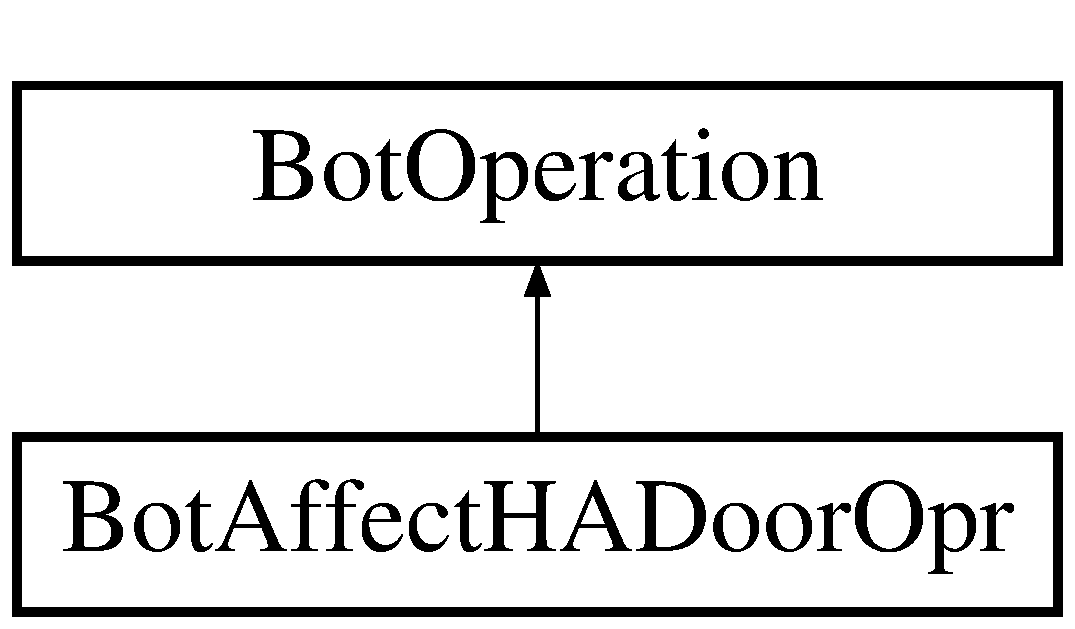
\includegraphics[height=2.000000cm]{classBotAffectHADoorOpr}
\end{center}
\end{figure}
\subsection*{Public Member Functions}
\begin{DoxyCompactItemize}
\item 
\hypertarget{classBotAffectHADoorOpr_aaf986c676dad29e1c151df36e42f3fc3}{{\bfseries Bot\-Affect\-H\-A\-Door\-Opr} (const std\-::string p\-Code, const int p\-Door\-Number, const int p\-Action)}\label{classBotAffectHADoorOpr_aaf986c676dad29e1c151df36e42f3fc3}

\item 
homebot\-::\-H\-A\-Door\-::\-Request \hyperlink{classBotAffectHADoorOpr_a25eed68370708f33963cb962b8e23580}{details} ()
\begin{DoxyCompactList}\small\item\em Provides access to operation details for testing purposes. \end{DoxyCompactList}\item 
bool \hyperlink{classBotAffectHADoorOpr_a6a82af8cbb0f8c48abbc04dc3f63811b}{is\-Executable} (const \hyperlink{classOperationParameters}{Operation\-Parameters} \&op\-Params)
\begin{DoxyCompactList}\small\item\em Validates that an operation is within acceptable parameters. \end{DoxyCompactList}\item 
bool \hyperlink{classBotAffectHADoorOpr_ae6ea9d64ffdb7f2c5622500109a545b7}{execute} (\hyperlink{classBotOprClients}{Bot\-Opr\-Clients} \&clients)
\begin{DoxyCompactList}\small\item\em Performs the behavior embedded in this operation (H\-A\-Door opens/closes doors via the Home Automation system) \end{DoxyCompactList}\end{DoxyCompactItemize}
\subsection*{Additional Inherited Members}


\subsection{Detailed Description}
Provides a Home Automation \char`\"{}door\char`\"{} operation (open/close); derived from \hyperlink{classBotOperation}{Bot\-Operation}. 

\subsection{Member Function Documentation}
\hypertarget{classBotAffectHADoorOpr_a25eed68370708f33963cb962b8e23580}{\index{Bot\-Affect\-H\-A\-Door\-Opr@{Bot\-Affect\-H\-A\-Door\-Opr}!details@{details}}
\index{details@{details}!BotAffectHADoorOpr@{Bot\-Affect\-H\-A\-Door\-Opr}}
\subsubsection[{details}]{\setlength{\rightskip}{0pt plus 5cm}homebot\-::\-H\-A\-Door\-::\-Request Bot\-Affect\-H\-A\-Door\-Opr\-::details (
\begin{DoxyParamCaption}
{}
\end{DoxyParamCaption}
)}}\label{classBotAffectHADoorOpr_a25eed68370708f33963cb962b8e23580}


Provides access to operation details for testing purposes. 

\begin{DoxyReturn}{Returns}
request formatted according to the R\-O\-S service definition for H\-A\-Door 
\end{DoxyReturn}
\hypertarget{classBotAffectHADoorOpr_ae6ea9d64ffdb7f2c5622500109a545b7}{\index{Bot\-Affect\-H\-A\-Door\-Opr@{Bot\-Affect\-H\-A\-Door\-Opr}!execute@{execute}}
\index{execute@{execute}!BotAffectHADoorOpr@{Bot\-Affect\-H\-A\-Door\-Opr}}
\subsubsection[{execute}]{\setlength{\rightskip}{0pt plus 5cm}bool Bot\-Affect\-H\-A\-Door\-Opr\-::execute (
\begin{DoxyParamCaption}
\item[{{\bf Bot\-Opr\-Clients} \&}]{clients}
\end{DoxyParamCaption}
)\hspace{0.3cm}{\ttfamily [virtual]}}}\label{classBotAffectHADoorOpr_ae6ea9d64ffdb7f2c5622500109a545b7}


Performs the behavior embedded in this operation (H\-A\-Door opens/closes doors via the Home Automation system) 


\begin{DoxyParams}[1]{Parameters}
\mbox{\tt in}  & {\em clients} & object containing the action/service clients used by Bot\-Operations to carry out their function \\
\hline
\end{DoxyParams}
\begin{DoxyReturn}{Returns}
bool indicating whether the operation executed successfully 
\end{DoxyReturn}


Reimplemented from \hyperlink{classBotOperation_ae1e806e3c0044dc0177e73a7d05711ba}{Bot\-Operation}.

\hypertarget{classBotAffectHADoorOpr_a6a82af8cbb0f8c48abbc04dc3f63811b}{\index{Bot\-Affect\-H\-A\-Door\-Opr@{Bot\-Affect\-H\-A\-Door\-Opr}!is\-Executable@{is\-Executable}}
\index{is\-Executable@{is\-Executable}!BotAffectHADoorOpr@{Bot\-Affect\-H\-A\-Door\-Opr}}
\subsubsection[{is\-Executable}]{\setlength{\rightskip}{0pt plus 5cm}bool Bot\-Affect\-H\-A\-Door\-Opr\-::is\-Executable (
\begin{DoxyParamCaption}
\item[{const {\bf Operation\-Parameters} \&}]{op\-Params}
\end{DoxyParamCaption}
)\hspace{0.3cm}{\ttfamily [virtual]}}}\label{classBotAffectHADoorOpr_a6a82af8cbb0f8c48abbc04dc3f63811b}


Validates that an operation is within acceptable parameters. 


\begin{DoxyParams}[1]{Parameters}
\mbox{\tt in}  & {\em op\-Params} & provides operational parameters for the system used to verify this operation can execute \\
\hline
\end{DoxyParams}
\begin{DoxyReturn}{Returns}
bool value indicating whether this operation can execute within the current Home\-Bot system 
\end{DoxyReturn}


Reimplemented from \hyperlink{classBotOperation_a0ed080d4c88b9ee0422666de169fb4a6}{Bot\-Operation}.



The documentation for this class was generated from the following files\-:\begin{DoxyCompactItemize}
\item 
include/homebot/\hyperlink{BotAffectHADoorOpr_8hpp}{Bot\-Affect\-H\-A\-Door\-Opr.\-hpp}\item 
src/\hyperlink{BotAffectHADoorOpr_8cpp}{Bot\-Affect\-H\-A\-Door\-Opr.\-cpp}\end{DoxyCompactItemize}

\hypertarget{classBotAffectHASceneOpr}{\section{Bot\-Affect\-H\-A\-Scene\-Opr Class Reference}
\label{classBotAffectHASceneOpr}\index{Bot\-Affect\-H\-A\-Scene\-Opr@{Bot\-Affect\-H\-A\-Scene\-Opr}}
}


Provides a home Automation \char`\"{}scene\char`\"{} (lighting) operation (turnon/turnoff); derived from \hyperlink{classBotOperation}{Bot\-Operation}.  




{\ttfamily \#include $<$Bot\-Affect\-H\-A\-Scene\-Opr.\-hpp$>$}

Inheritance diagram for Bot\-Affect\-H\-A\-Scene\-Opr\-:\begin{figure}[H]
\begin{center}
\leavevmode
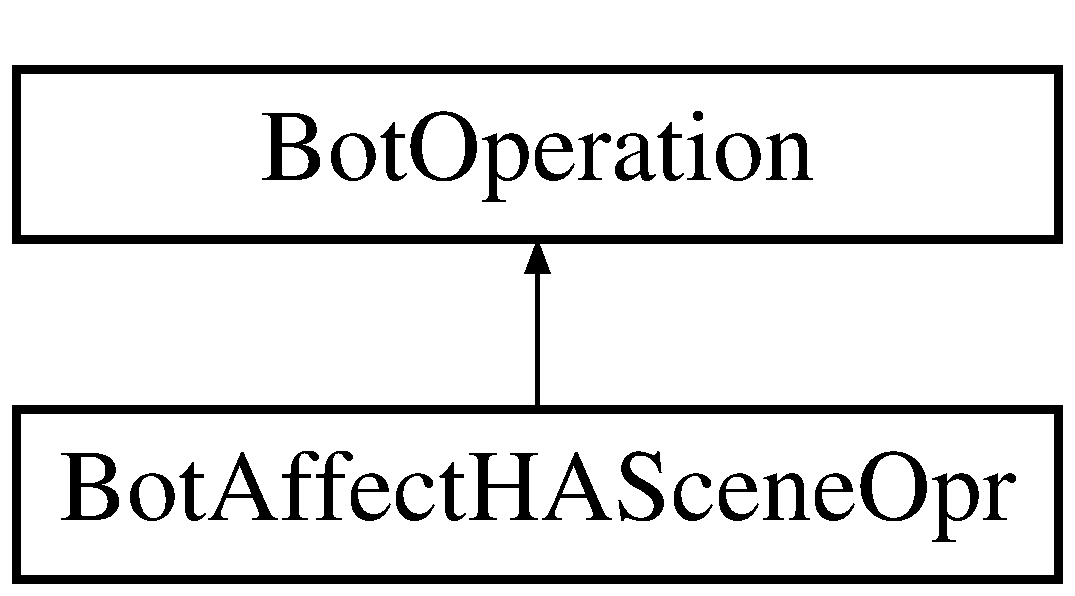
\includegraphics[height=2.000000cm]{classBotAffectHASceneOpr}
\end{center}
\end{figure}
\subsection*{Public Member Functions}
\begin{DoxyCompactItemize}
\item 
\hypertarget{classBotAffectHASceneOpr_a5564fd349eeefe4f1ee96a06de755f4e}{\hyperlink{classBotAffectHASceneOpr_a5564fd349eeefe4f1ee96a06de755f4e}{Bot\-Affect\-H\-A\-Scene\-Opr} ()}\label{classBotAffectHASceneOpr_a5564fd349eeefe4f1ee96a06de755f4e}

\begin{DoxyCompactList}\small\item\em Constructor with no arguments for \hyperlink{classBotAffectHASceneOpr}{Bot\-Affect\-H\-A\-Scene\-Opr}; creates a useless object that won't execute. \end{DoxyCompactList}\item 
\hyperlink{classBotAffectHASceneOpr_a7b924f64c28de823aae0591ac9b0d6ff}{Bot\-Affect\-H\-A\-Scene\-Opr} (const std\-::string p\-Code, const int p\-Scene\-Number, const int p\-Action)
\begin{DoxyCompactList}\small\item\em Constructor for \hyperlink{classBotAffectHASceneOpr}{Bot\-Affect\-H\-A\-Scene\-Opr}; builds operation that may execute. \end{DoxyCompactList}\item 
homebot\-::\-H\-A\-Scene\-::\-Request \hyperlink{classBotAffectHASceneOpr_a78d554b4969e6d1f64cd5b812662153b}{details} ()
\begin{DoxyCompactList}\small\item\em Provides access to operation details for testing purposes. \end{DoxyCompactList}\item 
bool \hyperlink{classBotAffectHASceneOpr_ada2804cb3287adacbfe0c1d5015842c8}{is\-Executable} (const \hyperlink{classOperationParameters}{Operation\-Parameters} \&op\-Params)
\begin{DoxyCompactList}\small\item\em Validates that an operation is within acceptable parameters. \end{DoxyCompactList}\item 
bool \hyperlink{classBotAffectHASceneOpr_a1ea965477504ea6a7e3d7c89ced15b3b}{execute} (\hyperlink{classBotOprClients}{Bot\-Opr\-Clients} \&clients)
\begin{DoxyCompactList}\small\item\em Performs the behavior embedded in this operation (H\-A\-Scene turnon/turnoff via the Home Automation system. \end{DoxyCompactList}\end{DoxyCompactItemize}
\subsection*{Additional Inherited Members}


\subsection{Detailed Description}
Provides a home Automation \char`\"{}scene\char`\"{} (lighting) operation (turnon/turnoff); derived from \hyperlink{classBotOperation}{Bot\-Operation}. 

\subsection{Constructor \& Destructor Documentation}
\hypertarget{classBotAffectHASceneOpr_a7b924f64c28de823aae0591ac9b0d6ff}{\index{Bot\-Affect\-H\-A\-Scene\-Opr@{Bot\-Affect\-H\-A\-Scene\-Opr}!Bot\-Affect\-H\-A\-Scene\-Opr@{Bot\-Affect\-H\-A\-Scene\-Opr}}
\index{Bot\-Affect\-H\-A\-Scene\-Opr@{Bot\-Affect\-H\-A\-Scene\-Opr}!BotAffectHASceneOpr@{Bot\-Affect\-H\-A\-Scene\-Opr}}
\subsubsection[{Bot\-Affect\-H\-A\-Scene\-Opr}]{\setlength{\rightskip}{0pt plus 5cm}Bot\-Affect\-H\-A\-Scene\-Opr\-::\-Bot\-Affect\-H\-A\-Scene\-Opr (
\begin{DoxyParamCaption}
\item[{const std\-::string}]{p\-Code, }
\item[{const int}]{p\-Scene\-Number, }
\item[{const int}]{p\-Action}
\end{DoxyParamCaption}
)}}\label{classBotAffectHASceneOpr_a7b924f64c28de823aae0591ac9b0d6ff}


Constructor for \hyperlink{classBotAffectHASceneOpr}{Bot\-Affect\-H\-A\-Scene\-Opr}; builds operation that may execute. 


\begin{DoxyParams}{Parameters}
{\em p\-Code} & std\-::string indicating operation code; must be H\-A\-Scene for this to execute \\
\hline
{\em p\-Scene\-Number} & integer for scene number to act on; must be within operational parameters to execute \\
\hline
{\em p\-Action} & integer for action to take; must be valid action for this to execute \\
\hline
\end{DoxyParams}


\subsection{Member Function Documentation}
\hypertarget{classBotAffectHASceneOpr_a78d554b4969e6d1f64cd5b812662153b}{\index{Bot\-Affect\-H\-A\-Scene\-Opr@{Bot\-Affect\-H\-A\-Scene\-Opr}!details@{details}}
\index{details@{details}!BotAffectHASceneOpr@{Bot\-Affect\-H\-A\-Scene\-Opr}}
\subsubsection[{details}]{\setlength{\rightskip}{0pt plus 5cm}homebot\-::\-H\-A\-Scene\-::\-Request Bot\-Affect\-H\-A\-Scene\-Opr\-::details (
\begin{DoxyParamCaption}
{}
\end{DoxyParamCaption}
)}}\label{classBotAffectHASceneOpr_a78d554b4969e6d1f64cd5b812662153b}


Provides access to operation details for testing purposes. 

\begin{DoxyReturn}{Returns}
request formatted according to the R\-O\-S service definition for H\-A\-Scene 
\end{DoxyReturn}
\hypertarget{classBotAffectHASceneOpr_a1ea965477504ea6a7e3d7c89ced15b3b}{\index{Bot\-Affect\-H\-A\-Scene\-Opr@{Bot\-Affect\-H\-A\-Scene\-Opr}!execute@{execute}}
\index{execute@{execute}!BotAffectHASceneOpr@{Bot\-Affect\-H\-A\-Scene\-Opr}}
\subsubsection[{execute}]{\setlength{\rightskip}{0pt plus 5cm}bool Bot\-Affect\-H\-A\-Scene\-Opr\-::execute (
\begin{DoxyParamCaption}
\item[{{\bf Bot\-Opr\-Clients} \&}]{clients}
\end{DoxyParamCaption}
)\hspace{0.3cm}{\ttfamily [virtual]}}}\label{classBotAffectHASceneOpr_a1ea965477504ea6a7e3d7c89ced15b3b}


Performs the behavior embedded in this operation (H\-A\-Scene turnon/turnoff via the Home Automation system. 


\begin{DoxyParams}[1]{Parameters}
\mbox{\tt in}  & {\em clients} & object containing the action/service clients used by Bot\-Operations to carry out their functions \\
\hline
\end{DoxyParams}
\begin{DoxyReturn}{Returns}
bool indicating whetherthe operation executed successfully 
\end{DoxyReturn}


Reimplemented from \hyperlink{classBotOperation_ae1e806e3c0044dc0177e73a7d05711ba}{Bot\-Operation}.

\hypertarget{classBotAffectHASceneOpr_ada2804cb3287adacbfe0c1d5015842c8}{\index{Bot\-Affect\-H\-A\-Scene\-Opr@{Bot\-Affect\-H\-A\-Scene\-Opr}!is\-Executable@{is\-Executable}}
\index{is\-Executable@{is\-Executable}!BotAffectHASceneOpr@{Bot\-Affect\-H\-A\-Scene\-Opr}}
\subsubsection[{is\-Executable}]{\setlength{\rightskip}{0pt plus 5cm}bool Bot\-Affect\-H\-A\-Scene\-Opr\-::is\-Executable (
\begin{DoxyParamCaption}
\item[{const {\bf Operation\-Parameters} \&}]{op\-Params}
\end{DoxyParamCaption}
)\hspace{0.3cm}{\ttfamily [virtual]}}}\label{classBotAffectHASceneOpr_ada2804cb3287adacbfe0c1d5015842c8}


Validates that an operation is within acceptable parameters. 


\begin{DoxyParams}[1]{Parameters}
\mbox{\tt in}  & {\em op\-Params} & provides oprational parameters for the system used to verify this operation can execute \\
\hline
\end{DoxyParams}
\begin{DoxyReturn}{Returns}
bool value indicating whether this operation can execute within the current Home\-Bot system 
\end{DoxyReturn}


Reimplemented from \hyperlink{classBotOperation_a0ed080d4c88b9ee0422666de169fb4a6}{Bot\-Operation}.



The documentation for this class was generated from the following files\-:\begin{DoxyCompactItemize}
\item 
include/homebot/\hyperlink{BotAffectHASceneOpr_8hpp}{Bot\-Affect\-H\-A\-Scene\-Opr.\-hpp}\item 
src/Bot\-Affect\-H\-A\-Scene\-Opr.\-cpp\end{DoxyCompactItemize}

\hypertarget{classBotAffectHAShadeOpr}{\section{Bot\-Affect\-H\-A\-Shade\-Opr Class Reference}
\label{classBotAffectHAShadeOpr}\index{Bot\-Affect\-H\-A\-Shade\-Opr@{Bot\-Affect\-H\-A\-Shade\-Opr}}
}


Provides a Home Automation \char`\"{}shade\char`\"{} operation (lower/raise); derived from \hyperlink{classBotOperation}{Bot\-Operation}.  




{\ttfamily \#include $<$Bot\-Affect\-H\-A\-Shade\-Opr.\-hpp$>$}

Inheritance diagram for Bot\-Affect\-H\-A\-Shade\-Opr\-:\begin{figure}[H]
\begin{center}
\leavevmode
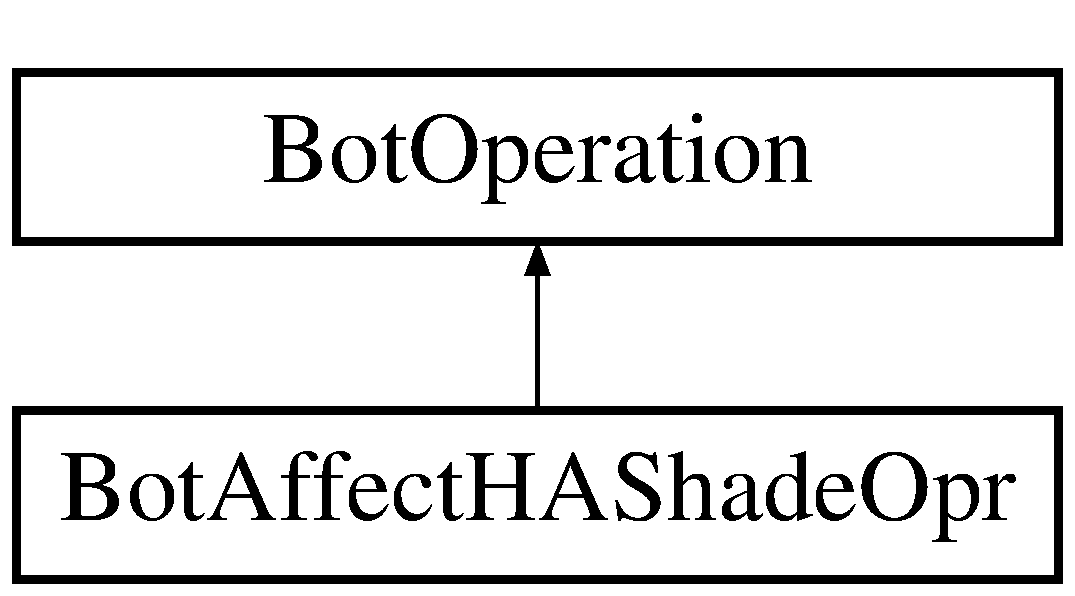
\includegraphics[height=2.000000cm]{classBotAffectHAShadeOpr}
\end{center}
\end{figure}
\subsection*{Public Member Functions}
\begin{DoxyCompactItemize}
\item 
\hypertarget{classBotAffectHAShadeOpr_afb5fe3fd27fb2c560d880091418b753f}{\hyperlink{classBotAffectHAShadeOpr_afb5fe3fd27fb2c560d880091418b753f}{Bot\-Affect\-H\-A\-Shade\-Opr} ()}\label{classBotAffectHAShadeOpr_afb5fe3fd27fb2c560d880091418b753f}

\begin{DoxyCompactList}\small\item\em Constructor with no arguments for \hyperlink{classBotAffectHAShadeOpr}{Bot\-Affect\-H\-A\-Shade\-Opr}; creates a useless object that won't execute. \end{DoxyCompactList}\item 
\hyperlink{classBotAffectHAShadeOpr_a84f68ccbc995adb8bcb8bb06c2c615ee}{Bot\-Affect\-H\-A\-Shade\-Opr} (const std\-::string p\-Code, const int p\-Shade\-Number, const int p\-Action)
\begin{DoxyCompactList}\small\item\em Constructor for \hyperlink{classBotAffectHAShadeOpr}{Bot\-Affect\-H\-A\-Shade\-Opr}; builds operation that may execute. \end{DoxyCompactList}\item 
homebot\-::\-H\-A\-Shade\-::\-Request \hyperlink{classBotAffectHAShadeOpr_a45e3809806091e342492d66e8fade1a6}{details} ()
\begin{DoxyCompactList}\small\item\em Proides access tooperation details for testing purposes. \end{DoxyCompactList}\item 
bool \hyperlink{classBotAffectHAShadeOpr_af37862e410311c38fd41994c51138cf6}{is\-Executable} (const \hyperlink{classOperationParameters}{Operation\-Parameters} \&op\-Params)
\begin{DoxyCompactList}\small\item\em Validates that an operation is within acceptable parameters. \end{DoxyCompactList}\item 
bool \hyperlink{classBotAffectHAShadeOpr_aab37d71a095f66554ee9958057c71356}{execute} (\hyperlink{classBotOprClients}{Bot\-Opr\-Clients} \&clients)
\begin{DoxyCompactList}\small\item\em Performs the behavior embedded in this operation (H\-A\-Scene lower/raises shades via the Home Automation system) \end{DoxyCompactList}\end{DoxyCompactItemize}
\subsection*{Additional Inherited Members}


\subsection{Detailed Description}
Provides a Home Automation \char`\"{}shade\char`\"{} operation (lower/raise); derived from \hyperlink{classBotOperation}{Bot\-Operation}. 

\subsection{Constructor \& Destructor Documentation}
\hypertarget{classBotAffectHAShadeOpr_a84f68ccbc995adb8bcb8bb06c2c615ee}{\index{Bot\-Affect\-H\-A\-Shade\-Opr@{Bot\-Affect\-H\-A\-Shade\-Opr}!Bot\-Affect\-H\-A\-Shade\-Opr@{Bot\-Affect\-H\-A\-Shade\-Opr}}
\index{Bot\-Affect\-H\-A\-Shade\-Opr@{Bot\-Affect\-H\-A\-Shade\-Opr}!BotAffectHAShadeOpr@{Bot\-Affect\-H\-A\-Shade\-Opr}}
\subsubsection[{Bot\-Affect\-H\-A\-Shade\-Opr}]{\setlength{\rightskip}{0pt plus 5cm}Bot\-Affect\-H\-A\-Shade\-Opr\-::\-Bot\-Affect\-H\-A\-Shade\-Opr (
\begin{DoxyParamCaption}
\item[{const std\-::string}]{p\-Code, }
\item[{const int}]{p\-Shade\-Number, }
\item[{const int}]{p\-Action}
\end{DoxyParamCaption}
)}}\label{classBotAffectHAShadeOpr_a84f68ccbc995adb8bcb8bb06c2c615ee}


Constructor for \hyperlink{classBotAffectHAShadeOpr}{Bot\-Affect\-H\-A\-Shade\-Opr}; builds operation that may execute. 


\begin{DoxyParams}{Parameters}
{\em p\-Code} & std\-::string indicating operation code; must be H\-A\-Shade for this to execute \\
\hline
{\em p\-Shade\-Number} & integer for shade number to act on; must be within operational parameters to execute \\
\hline
{\em p\-Action} & integer for action to take; must be valid action for this to execute \\
\hline
\end{DoxyParams}


\subsection{Member Function Documentation}
\hypertarget{classBotAffectHAShadeOpr_a45e3809806091e342492d66e8fade1a6}{\index{Bot\-Affect\-H\-A\-Shade\-Opr@{Bot\-Affect\-H\-A\-Shade\-Opr}!details@{details}}
\index{details@{details}!BotAffectHAShadeOpr@{Bot\-Affect\-H\-A\-Shade\-Opr}}
\subsubsection[{details}]{\setlength{\rightskip}{0pt plus 5cm}homebot\-::\-H\-A\-Shade\-::\-Request Bot\-Affect\-H\-A\-Shade\-Opr\-::details (
\begin{DoxyParamCaption}
{}
\end{DoxyParamCaption}
)}}\label{classBotAffectHAShadeOpr_a45e3809806091e342492d66e8fade1a6}


Proides access tooperation details for testing purposes. 

\begin{DoxyReturn}{Returns}
request formated according to the R\-O\-S service definition for H\-A\-Shade 
\end{DoxyReturn}
\hypertarget{classBotAffectHAShadeOpr_aab37d71a095f66554ee9958057c71356}{\index{Bot\-Affect\-H\-A\-Shade\-Opr@{Bot\-Affect\-H\-A\-Shade\-Opr}!execute@{execute}}
\index{execute@{execute}!BotAffectHAShadeOpr@{Bot\-Affect\-H\-A\-Shade\-Opr}}
\subsubsection[{execute}]{\setlength{\rightskip}{0pt plus 5cm}bool Bot\-Affect\-H\-A\-Shade\-Opr\-::execute (
\begin{DoxyParamCaption}
\item[{{\bf Bot\-Opr\-Clients} \&}]{clients}
\end{DoxyParamCaption}
)\hspace{0.3cm}{\ttfamily [virtual]}}}\label{classBotAffectHAShadeOpr_aab37d71a095f66554ee9958057c71356}


Performs the behavior embedded in this operation (H\-A\-Scene lower/raises shades via the Home Automation system) 


\begin{DoxyParams}{Parameters}
{\em clients} & object containing the action/service clients used by Bot\-Operations to carry out their function \\
\hline
\end{DoxyParams}
\begin{DoxyReturn}{Returns}
bool indicating whether the operation executed successfully 
\end{DoxyReturn}


Reimplemented from \hyperlink{classBotOperation_ae1e806e3c0044dc0177e73a7d05711ba}{Bot\-Operation}.

\hypertarget{classBotAffectHAShadeOpr_af37862e410311c38fd41994c51138cf6}{\index{Bot\-Affect\-H\-A\-Shade\-Opr@{Bot\-Affect\-H\-A\-Shade\-Opr}!is\-Executable@{is\-Executable}}
\index{is\-Executable@{is\-Executable}!BotAffectHAShadeOpr@{Bot\-Affect\-H\-A\-Shade\-Opr}}
\subsubsection[{is\-Executable}]{\setlength{\rightskip}{0pt plus 5cm}bool Bot\-Affect\-H\-A\-Shade\-Opr\-::is\-Executable (
\begin{DoxyParamCaption}
\item[{const {\bf Operation\-Parameters} \&}]{op\-Params}
\end{DoxyParamCaption}
)\hspace{0.3cm}{\ttfamily [virtual]}}}\label{classBotAffectHAShadeOpr_af37862e410311c38fd41994c51138cf6}


Validates that an operation is within acceptable parameters. 


\begin{DoxyParams}[1]{Parameters}
\mbox{\tt in}  & {\em op\-Params} & provides operational parameters for the system used to verify this operation can execute \\
\hline
\end{DoxyParams}
\begin{DoxyReturn}{Returns}
bool value indicating whether this operation can execute within the current Home\-Bot system 
\end{DoxyReturn}


Reimplemented from \hyperlink{classBotOperation_a0ed080d4c88b9ee0422666de169fb4a6}{Bot\-Operation}.



The documentation for this class was generated from the following files\-:\begin{DoxyCompactItemize}
\item 
include/homebot/Bot\-Affect\-H\-A\-Shade\-Opr.\-hpp\item 
src/Bot\-Affect\-H\-A\-Shade\-Opr.\-cpp\end{DoxyCompactItemize}

\hypertarget{classBotBehavior}{\section{Bot\-Behavior Class Reference}
\label{classBotBehavior}\index{Bot\-Behavior@{Bot\-Behavior}}
}


Collection of operations used to perform a behavior.  




{\ttfamily \#include $<$Bot\-Behavior.\-hpp$>$}

\subsection*{Public Member Functions}
\begin{DoxyCompactItemize}
\item 
\hypertarget{classBotBehavior_a07b5a5aa8e4318002515477f1d1405c5}{{\bfseries Bot\-Behavior} (const std\-::string p\-Name, const \hyperlink{classOperationParameters}{Operation\-Parameters} \&p\-Op\-Params)}\label{classBotBehavior_a07b5a5aa8e4318002515477f1d1405c5}

\item 
std\-::string \hyperlink{classBotBehavior_a7a79661c4afeab6fee0388fe84c6c45a}{get\-Name} ()
\begin{DoxyCompactList}\small\item\em Provides access to the behavior's name. \end{DoxyCompactList}\item 
bool \hyperlink{classBotBehavior_a2814c74acdbb8e527b24d67de90d393d}{insert} (const std\-::string text\-Phased\-Opr)
\begin{DoxyCompactList}\small\item\em Adds an executable (transformed) operation to a phase of a behavior (phases are prelim(inary), main, and post) \end{DoxyCompactList}\item 
bool \hyperlink{classBotBehavior_aebab943aa7ebb3a8ea540d8eccf929e3}{perform\-Prelim} (\hyperlink{classBotOprClients}{Bot\-Opr\-Clients} \&opr\-Clients)
\begin{DoxyCompactList}\small\item\em Execute the operations in the preliminary phase of this behavior. \end{DoxyCompactList}\item 
bool \hyperlink{classBotBehavior_add170f17aa5aa70014bb5dd23d1f0f50}{perform\-Main} (\hyperlink{classBotOprClients}{Bot\-Opr\-Clients} \&opr\-Clients)
\begin{DoxyCompactList}\small\item\em Execute the operations in the main phase of this behavior. \end{DoxyCompactList}\item 
bool \hyperlink{classBotBehavior_a6326a763ff29158e41201b2957004b9b}{perform\-Post} (\hyperlink{classBotOprClients}{Bot\-Opr\-Clients} \&opr\-Clients)
\begin{DoxyCompactList}\small\item\em Execute the operations in the post phase of this behavior. \end{DoxyCompactList}\end{DoxyCompactItemize}


\subsection{Detailed Description}
Collection of operations used to perform a behavior. 

\subsection{Member Function Documentation}
\hypertarget{classBotBehavior_a7a79661c4afeab6fee0388fe84c6c45a}{\index{Bot\-Behavior@{Bot\-Behavior}!get\-Name@{get\-Name}}
\index{get\-Name@{get\-Name}!BotBehavior@{Bot\-Behavior}}
\subsubsection[{get\-Name}]{\setlength{\rightskip}{0pt plus 5cm}std\-::string Bot\-Behavior\-::get\-Name (
\begin{DoxyParamCaption}
{}
\end{DoxyParamCaption}
)}}\label{classBotBehavior_a7a79661c4afeab6fee0388fe84c6c45a}


Provides access to the behavior's name. 

\begin{DoxyReturn}{Returns}
string representing the behavior's name 
\end{DoxyReturn}
\hypertarget{classBotBehavior_a2814c74acdbb8e527b24d67de90d393d}{\index{Bot\-Behavior@{Bot\-Behavior}!insert@{insert}}
\index{insert@{insert}!BotBehavior@{Bot\-Behavior}}
\subsubsection[{insert}]{\setlength{\rightskip}{0pt plus 5cm}bool Bot\-Behavior\-::insert (
\begin{DoxyParamCaption}
\item[{const std\-::string}]{text\-Phased\-Opr}
\end{DoxyParamCaption}
)}}\label{classBotBehavior_a2814c74acdbb8e527b24d67de90d393d}


Adds an executable (transformed) operation to a phase of a behavior (phases are prelim(inary), main, and post) 


\begin{DoxyParams}[1]{Parameters}
\mbox{\tt in}  & {\em text\-Phased\-Opr} & containing an operation phase and an operation code and details \\
\hline
\end{DoxyParams}
\begin{DoxyReturn}{Returns}
bool indicating whether the operation was inserted successfully 
\end{DoxyReturn}
\hypertarget{classBotBehavior_add170f17aa5aa70014bb5dd23d1f0f50}{\index{Bot\-Behavior@{Bot\-Behavior}!perform\-Main@{perform\-Main}}
\index{perform\-Main@{perform\-Main}!BotBehavior@{Bot\-Behavior}}
\subsubsection[{perform\-Main}]{\setlength{\rightskip}{0pt plus 5cm}bool Bot\-Behavior\-::perform\-Main (
\begin{DoxyParamCaption}
\item[{{\bf Bot\-Opr\-Clients} \&}]{opr\-Clients}
\end{DoxyParamCaption}
)}}\label{classBotBehavior_add170f17aa5aa70014bb5dd23d1f0f50}


Execute the operations in the main phase of this behavior. 


\begin{DoxyParams}{Parameters}
{\em opr\-Clients} & object containing the action/service clients used by Bot\-Operations to carry out their function \\
\hline
\end{DoxyParams}
\begin{DoxyReturn}{Returns}
bool indicating whether the phase completed successfully 
\end{DoxyReturn}
\hypertarget{classBotBehavior_a6326a763ff29158e41201b2957004b9b}{\index{Bot\-Behavior@{Bot\-Behavior}!perform\-Post@{perform\-Post}}
\index{perform\-Post@{perform\-Post}!BotBehavior@{Bot\-Behavior}}
\subsubsection[{perform\-Post}]{\setlength{\rightskip}{0pt plus 5cm}bool Bot\-Behavior\-::perform\-Post (
\begin{DoxyParamCaption}
\item[{{\bf Bot\-Opr\-Clients} \&}]{opr\-Clients}
\end{DoxyParamCaption}
)}}\label{classBotBehavior_a6326a763ff29158e41201b2957004b9b}


Execute the operations in the post phase of this behavior. 


\begin{DoxyParams}{Parameters}
{\em opr\-Clients} & object containing the action/service clients used by Bot\-Operations to carry out their function \\
\hline
\end{DoxyParams}
\begin{DoxyReturn}{Returns}
bool indicating whether the phase completed successfully 
\end{DoxyReturn}
\hypertarget{classBotBehavior_aebab943aa7ebb3a8ea540d8eccf929e3}{\index{Bot\-Behavior@{Bot\-Behavior}!perform\-Prelim@{perform\-Prelim}}
\index{perform\-Prelim@{perform\-Prelim}!BotBehavior@{Bot\-Behavior}}
\subsubsection[{perform\-Prelim}]{\setlength{\rightskip}{0pt plus 5cm}bool Bot\-Behavior\-::perform\-Prelim (
\begin{DoxyParamCaption}
\item[{{\bf Bot\-Opr\-Clients} \&}]{opr\-Clients}
\end{DoxyParamCaption}
)}}\label{classBotBehavior_aebab943aa7ebb3a8ea540d8eccf929e3}


Execute the operations in the preliminary phase of this behavior. 


\begin{DoxyParams}{Parameters}
{\em opr\-Clients} & object containing the action/service clients used by Bot\-Operations to carry out their function \\
\hline
\end{DoxyParams}
\begin{DoxyReturn}{Returns}
bool indicating whether the phase completed successfully 
\end{DoxyReturn}


The documentation for this class was generated from the following files\-:\begin{DoxyCompactItemize}
\item 
include/homebot/\hyperlink{BotBehavior_8hpp}{Bot\-Behavior.\-hpp}\item 
src/\hyperlink{BotBehavior_8cpp}{Bot\-Behavior.\-cpp}\end{DoxyCompactItemize}

\hypertarget{classBotMoveBaseOpr}{\section{Bot\-Move\-Base\-Opr Class Reference}
\label{classBotMoveBaseOpr}\index{Bot\-Move\-Base\-Opr@{Bot\-Move\-Base\-Opr}}
}


Provides a service robot \char`\"{}move\-\_\-base\char`\"{} operation (move to frame\-\_\-id/\-Pose); derived from \hyperlink{classBotOperation}{Bot\-Operation}.  




{\ttfamily \#include $<$Bot\-Move\-Base\-Opr.\-hpp$>$}

Inheritance diagram for Bot\-Move\-Base\-Opr\-:\begin{figure}[H]
\begin{center}
\leavevmode
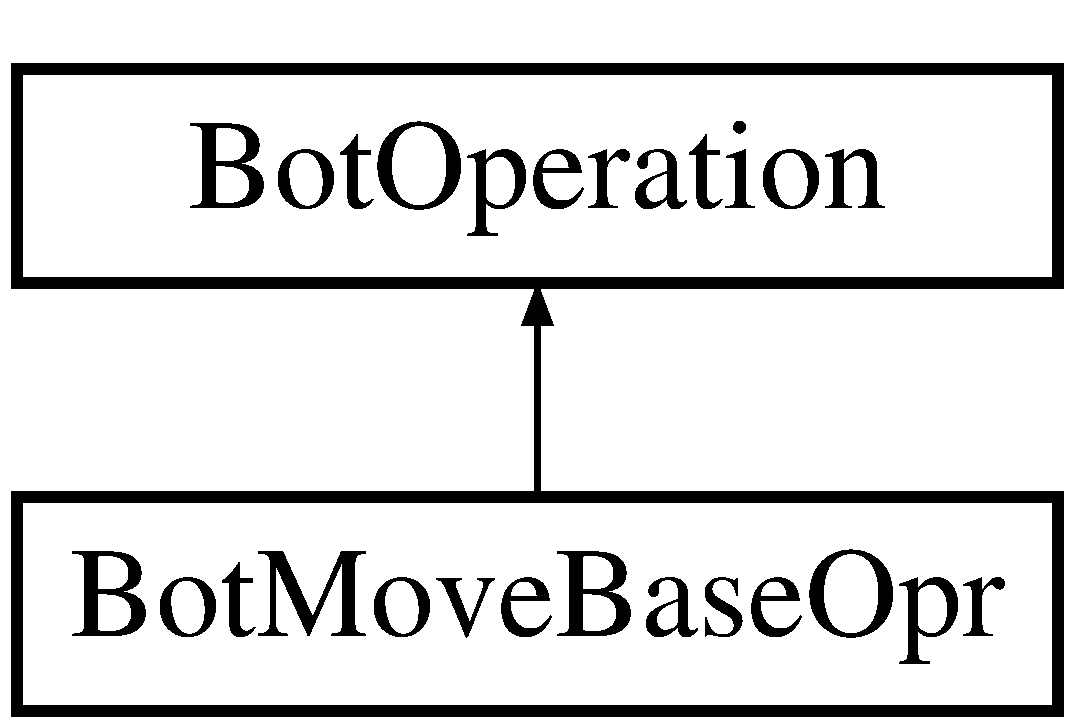
\includegraphics[height=2.000000cm]{classBotMoveBaseOpr}
\end{center}
\end{figure}
\subsection*{Public Member Functions}
\begin{DoxyCompactItemize}
\item 
\hypertarget{classBotMoveBaseOpr_a269ba342770db907481955adb5bd9cec}{{\bfseries Bot\-Move\-Base\-Opr} (const std\-::string p\-Code, const std\-::string p\-Frame\-\_\-id, const double p\-X\-Pos, const double p\-Y\-Pos, const double p\-Z\-Pos, const double p\-X\-Orient, const double p\-Y\-Orient, const double p\-Z\-Orient, const double p\-W\-Orient)}\label{classBotMoveBaseOpr_a269ba342770db907481955adb5bd9cec}

\item 
move\-\_\-base\-\_\-msgs\-::\-Move\-Base\-Goal \hyperlink{classBotMoveBaseOpr_ad03fb9f3398b557549408752690e7d58}{details} ()
\begin{DoxyCompactList}\small\item\em Provides access to operation details for testing purposes. \end{DoxyCompactList}\item 
bool \hyperlink{classBotMoveBaseOpr_ae6a4ed7325d3bc728b6934250171178d}{is\-Executable} (const \hyperlink{classOperationParameters}{Operation\-Parameters} \&op\-Params)
\begin{DoxyCompactList}\small\item\em Validates that an operation is within acceptable parameters. \end{DoxyCompactList}\item 
bool \hyperlink{classBotMoveBaseOpr_aebac9f650a9960e132dccc61e54b8c93}{execute} (\hyperlink{classBotOprClients}{Bot\-Opr\-Clients} \&clients)
\begin{DoxyCompactList}\small\item\em Performs the behavior embedded in this operation (Bot\-Move\-Base moves a robot base via its navigation system. \end{DoxyCompactList}\end{DoxyCompactItemize}
\subsection*{Additional Inherited Members}


\subsection{Detailed Description}
Provides a service robot \char`\"{}move\-\_\-base\char`\"{} operation (move to frame\-\_\-id/\-Pose); derived from \hyperlink{classBotOperation}{Bot\-Operation}. 

\subsection{Member Function Documentation}
\hypertarget{classBotMoveBaseOpr_ad03fb9f3398b557549408752690e7d58}{\index{Bot\-Move\-Base\-Opr@{Bot\-Move\-Base\-Opr}!details@{details}}
\index{details@{details}!BotMoveBaseOpr@{Bot\-Move\-Base\-Opr}}
\subsubsection[{details}]{\setlength{\rightskip}{0pt plus 5cm}move\-\_\-base\-\_\-msgs\-::\-Move\-Base\-Goal Bot\-Move\-Base\-Opr\-::details (
\begin{DoxyParamCaption}
{}
\end{DoxyParamCaption}
)}}\label{classBotMoveBaseOpr_ad03fb9f3398b557549408752690e7d58}


Provides access to operation details for testing purposes. 

\begin{DoxyReturn}{Returns}
goal formatted according to the R\-O\-S action definition for Move\-Base 
\end{DoxyReturn}
\hypertarget{classBotMoveBaseOpr_aebac9f650a9960e132dccc61e54b8c93}{\index{Bot\-Move\-Base\-Opr@{Bot\-Move\-Base\-Opr}!execute@{execute}}
\index{execute@{execute}!BotMoveBaseOpr@{Bot\-Move\-Base\-Opr}}
\subsubsection[{execute}]{\setlength{\rightskip}{0pt plus 5cm}bool Bot\-Move\-Base\-Opr\-::execute (
\begin{DoxyParamCaption}
\item[{{\bf Bot\-Opr\-Clients} \&}]{clients}
\end{DoxyParamCaption}
)\hspace{0.3cm}{\ttfamily [virtual]}}}\label{classBotMoveBaseOpr_aebac9f650a9960e132dccc61e54b8c93}


Performs the behavior embedded in this operation (Bot\-Move\-Base moves a robot base via its navigation system. 


\begin{DoxyParams}[1]{Parameters}
\mbox{\tt in}  & {\em clients} & object containing the action/service clients used by Bot\-Operations to carry out their function \\
\hline
\end{DoxyParams}
\begin{DoxyReturn}{Returns}
bool indicating whether the operation executed successfully 
\end{DoxyReturn}


Reimplemented from \hyperlink{classBotOperation_ae1e806e3c0044dc0177e73a7d05711ba}{Bot\-Operation}.

\hypertarget{classBotMoveBaseOpr_ae6a4ed7325d3bc728b6934250171178d}{\index{Bot\-Move\-Base\-Opr@{Bot\-Move\-Base\-Opr}!is\-Executable@{is\-Executable}}
\index{is\-Executable@{is\-Executable}!BotMoveBaseOpr@{Bot\-Move\-Base\-Opr}}
\subsubsection[{is\-Executable}]{\setlength{\rightskip}{0pt plus 5cm}bool Bot\-Move\-Base\-Opr\-::is\-Executable (
\begin{DoxyParamCaption}
\item[{const {\bf Operation\-Parameters} \&}]{op\-Params}
\end{DoxyParamCaption}
)\hspace{0.3cm}{\ttfamily [virtual]}}}\label{classBotMoveBaseOpr_ae6a4ed7325d3bc728b6934250171178d}


Validates that an operation is within acceptable parameters. 


\begin{DoxyParams}[1]{Parameters}
\mbox{\tt in}  & {\em op\-Params} & provides operational parameters for the system used to verify this operation can execute \\
\hline
\end{DoxyParams}
\begin{DoxyReturn}{Returns}
bool value indicating whether this operation can execute within the current Home\-Bot system 
\end{DoxyReturn}


Reimplemented from \hyperlink{classBotOperation_a0ed080d4c88b9ee0422666de169fb4a6}{Bot\-Operation}.



The documentation for this class was generated from the following files\-:\begin{DoxyCompactItemize}
\item 
include/homebot/\hyperlink{BotMoveBaseOpr_8hpp}{Bot\-Move\-Base\-Opr.\-hpp}\item 
src/\hyperlink{BotMoveBaseOpr_8cpp}{Bot\-Move\-Base\-Opr.\-cpp}\end{DoxyCompactItemize}

\hypertarget{classBotOperation}{\section{Bot\-Operation Class Reference}
\label{classBotOperation}\index{Bot\-Operation@{Bot\-Operation}}
}


Base class for all operations; used to create new instances of derived classes from text-\/based source.  




{\ttfamily \#include $<$Bot\-Operation.\-hpp$>$}

Inheritance diagram for Bot\-Operation\-:\begin{figure}[H]
\begin{center}
\leavevmode
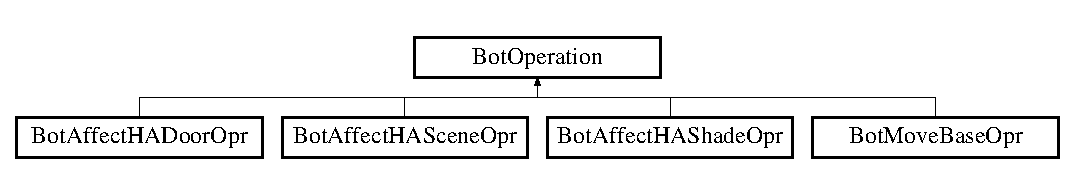
\includegraphics[height=1.891892cm]{classBotOperation}
\end{center}
\end{figure}
\subsection*{Public Member Functions}
\begin{DoxyCompactItemize}
\item 
\hypertarget{classBotOperation_a05997cf0f5d8b6d8a0621f6ccfd463ae}{{\bfseries Bot\-Operation} (const std\-::string p\-Raw\-Text)}\label{classBotOperation_a05997cf0f5d8b6d8a0621f6ccfd463ae}

\item 
\hypertarget{classBotOperation_a4acc1fc67e0bbbbda2df061c77b67bfa}{{\bfseries Bot\-Operation} (const std\-::string p\-Raw\-Text, const std\-::string p\-Code)}\label{classBotOperation_a4acc1fc67e0bbbbda2df061c77b67bfa}

\item 
std\-::string \hyperlink{classBotOperation_a768d7dabd43ccbabb72c4ed10dd98ffa}{get\-Code} ()
\begin{DoxyCompactList}\small\item\em Provides access to the code in an operation through the base class -\/ primarily for testing purposes. \end{DoxyCompactList}\item 
\hypertarget{classBotOperation_af178b91062e8844822122599331dfd0b}{std\-::string {\bfseries get\-Raw\-Text} ()}\label{classBotOperation_af178b91062e8844822122599331dfd0b}

\item 
virtual bool \hyperlink{classBotOperation_a0ed080d4c88b9ee0422666de169fb4a6}{is\-Executable} (const \hyperlink{classOperationParameters}{Operation\-Parameters} \&op\-Params)
\begin{DoxyCompactList}\small\item\em Determine as closely as possible whether an operation is valid (can be executed) \end{DoxyCompactList}\item 
virtual bool \hyperlink{classBotOperation_ae1e806e3c0044dc0177e73a7d05711ba}{execute} (\hyperlink{classBotOprClients}{Bot\-Opr\-Clients} \&clients)
\begin{DoxyCompactList}\small\item\em \hyperlink{classBotOperation}{Bot\-Operation} objects are self-\/executing themselves; but a base class object should not be executed. \end{DoxyCompactList}\item 
boost\-::shared\-\_\-ptr$<$ \hyperlink{classBotOperation}{Bot\-Operation} $>$ \hyperlink{classBotOperation_a894e399d0cc8e564831dc4cecd363c09}{transform} (const \hyperlink{classOperationParameters}{Operation\-Parameters} \&op\-Params)
\begin{DoxyCompactList}\small\item\em Base class method to construct a derived class object from source text (inserted by constructor) \end{DoxyCompactList}\end{DoxyCompactItemize}
\subsection*{Protected Attributes}
\begin{DoxyCompactItemize}
\item 
\hypertarget{classBotOperation_ae5b6b68a246f5d55b67f0f26939a5f95}{std\-::string {\bfseries code}}\label{classBotOperation_ae5b6b68a246f5d55b67f0f26939a5f95}

\item 
\hypertarget{classBotOperation_a256d5a82958cdd1f00d441c2e5ae6a37}{std\-::string {\bfseries raw\-Text}}\label{classBotOperation_a256d5a82958cdd1f00d441c2e5ae6a37}

\end{DoxyCompactItemize}


\subsection{Detailed Description}
Base class for all operations; used to create new instances of derived classes from text-\/based source. 

\subsection{Member Function Documentation}
\hypertarget{classBotOperation_ae1e806e3c0044dc0177e73a7d05711ba}{\index{Bot\-Operation@{Bot\-Operation}!execute@{execute}}
\index{execute@{execute}!BotOperation@{Bot\-Operation}}
\subsubsection[{execute}]{\setlength{\rightskip}{0pt plus 5cm}bool Bot\-Operation\-::execute (
\begin{DoxyParamCaption}
\item[{{\bf Bot\-Opr\-Clients} \&}]{clients}
\end{DoxyParamCaption}
)\hspace{0.3cm}{\ttfamily [virtual]}}}\label{classBotOperation_ae1e806e3c0044dc0177e73a7d05711ba}


\hyperlink{classBotOperation}{Bot\-Operation} objects are self-\/executing themselves; but a base class object should not be executed. 


\begin{DoxyParams}[1]{Parameters}
\mbox{\tt in}  & {\em \hyperlink{classBotOprClients}{Bot\-Opr\-Clients}} & clients to use for executing the operation \\
\hline
\end{DoxyParams}
\begin{DoxyReturn}{Returns}
bool indication of whether the execution was successful (true) or not (false) 
\end{DoxyReturn}


Reimplemented in \hyperlink{classBotMoveBaseOpr_aebac9f650a9960e132dccc61e54b8c93}{Bot\-Move\-Base\-Opr}, \hyperlink{classBotAffectHADoorOpr_ae6ea9d64ffdb7f2c5622500109a545b7}{Bot\-Affect\-H\-A\-Door\-Opr}, \hyperlink{classBotAffectHASceneOpr_a1ea965477504ea6a7e3d7c89ced15b3b}{Bot\-Affect\-H\-A\-Scene\-Opr}, and \hyperlink{classBotAffectHAShadeOpr_aab37d71a095f66554ee9958057c71356}{Bot\-Affect\-H\-A\-Shade\-Opr}.

\hypertarget{classBotOperation_a768d7dabd43ccbabb72c4ed10dd98ffa}{\index{Bot\-Operation@{Bot\-Operation}!get\-Code@{get\-Code}}
\index{get\-Code@{get\-Code}!BotOperation@{Bot\-Operation}}
\subsubsection[{get\-Code}]{\setlength{\rightskip}{0pt plus 5cm}std\-::string Bot\-Operation\-::get\-Code (
\begin{DoxyParamCaption}
{}
\end{DoxyParamCaption}
)}}\label{classBotOperation_a768d7dabd43ccbabb72c4ed10dd98ffa}


Provides access to the code in an operation through the base class -\/ primarily for testing purposes. 

\begin{DoxyReturn}{Returns}
std\-::string code from this object 
\end{DoxyReturn}
\hypertarget{classBotOperation_a0ed080d4c88b9ee0422666de169fb4a6}{\index{Bot\-Operation@{Bot\-Operation}!is\-Executable@{is\-Executable}}
\index{is\-Executable@{is\-Executable}!BotOperation@{Bot\-Operation}}
\subsubsection[{is\-Executable}]{\setlength{\rightskip}{0pt plus 5cm}bool Bot\-Operation\-::is\-Executable (
\begin{DoxyParamCaption}
\item[{const {\bf Operation\-Parameters} \&}]{op\-Params}
\end{DoxyParamCaption}
)\hspace{0.3cm}{\ttfamily [virtual]}}}\label{classBotOperation_a0ed080d4c88b9ee0422666de169fb4a6}


Determine as closely as possible whether an operation is valid (can be executed) 


\begin{DoxyParams}[1]{Parameters}
\mbox{\tt in}  & {\em \hyperlink{classOperationParameters}{Operation\-Parameters}} & op\-Params that assist with validation \\
\hline
\end{DoxyParams}
\begin{DoxyReturn}{Returns}
bool value that indicates whether the operation can be executed 
\end{DoxyReturn}


Reimplemented in \hyperlink{classBotMoveBaseOpr_ae6a4ed7325d3bc728b6934250171178d}{Bot\-Move\-Base\-Opr}, \hyperlink{classBotAffectHADoorOpr_a6a82af8cbb0f8c48abbc04dc3f63811b}{Bot\-Affect\-H\-A\-Door\-Opr}, \hyperlink{classBotAffectHASceneOpr_ada2804cb3287adacbfe0c1d5015842c8}{Bot\-Affect\-H\-A\-Scene\-Opr}, and \hyperlink{classBotAffectHAShadeOpr_af37862e410311c38fd41994c51138cf6}{Bot\-Affect\-H\-A\-Shade\-Opr}.

\hypertarget{classBotOperation_a894e399d0cc8e564831dc4cecd363c09}{\index{Bot\-Operation@{Bot\-Operation}!transform@{transform}}
\index{transform@{transform}!BotOperation@{Bot\-Operation}}
\subsubsection[{transform}]{\setlength{\rightskip}{0pt plus 5cm}boost\-::shared\-\_\-ptr$<$ {\bf Bot\-Operation} $>$ Bot\-Operation\-::transform (
\begin{DoxyParamCaption}
\item[{const {\bf Operation\-Parameters} \&}]{op\-Params}
\end{DoxyParamCaption}
)}}\label{classBotOperation_a894e399d0cc8e564831dc4cecd363c09}


Base class method to construct a derived class object from source text (inserted by constructor) 


\begin{DoxyParams}[1]{Parameters}
\mbox{\tt in}  & {\em op\-Params} & provides operational parameters for the system used to verify this operation \\
\hline
\end{DoxyParams}
\begin{DoxyReturn}{Returns}
boost\-::shared\-\_\-ptr$<$\-Bot\-Operation$>$ for the derived class object (non-\/executable base object returned if transformation failed) 
\end{DoxyReturn}


The documentation for this class was generated from the following files\-:\begin{DoxyCompactItemize}
\item 
include/homebot/\hyperlink{BotOperation_8hpp}{Bot\-Operation.\-hpp}\item 
src/\hyperlink{BotOperation_8cpp}{Bot\-Operation.\-cpp}\end{DoxyCompactItemize}

\hypertarget{classBotOprClients}{\section{Bot\-Opr\-Clients Class Reference}
\label{classBotOprClients}\index{Bot\-Opr\-Clients@{Bot\-Opr\-Clients}}
}


An object to hold R\-O\-S action/service clients needed to perform Bot operations in the Home\-Bot system.  




{\ttfamily \#include $<$Bot\-Opr\-Clients.\-hpp$>$}

\subsection*{Public Member Functions}
\begin{DoxyCompactItemize}
\item 
\hypertarget{classBotOprClients_a536678010c6da735d24be3c3f3c08591}{\hyperlink{classBotOprClients_a536678010c6da735d24be3c3f3c08591}{Bot\-Opr\-Clients} ()}\label{classBotOprClients_a536678010c6da735d24be3c3f3c08591}

\begin{DoxyCompactList}\small\item\em Constructor for \hyperlink{classBotOprClients}{Bot\-Opr\-Clients}; calling this constructor creates a series of service and action clients. \end{DoxyCompactList}\item 
bool \hyperlink{classBotOprClients_a391df41704d4984c1c757c4e095a5fe7}{all\-Started} ()
\begin{DoxyCompactList}\small\item\em Provide status as to whether all of the clients are started (based on whether the services are available) \end{DoxyCompactList}\end{DoxyCompactItemize}
\subsection*{Friends}
\begin{DoxyCompactItemize}
\item 
\hypertarget{classBotOprClients_a444222e47c36e1fec1177b4946f76f31}{class {\bfseries Bot\-Affect\-H\-A\-Door\-Opr}}\label{classBotOprClients_a444222e47c36e1fec1177b4946f76f31}

\item 
\hypertarget{classBotOprClients_a108beaf6fe53a7d3162abe84d250afb9}{class {\bfseries Bot\-Affect\-H\-A\-Scene\-Opr}}\label{classBotOprClients_a108beaf6fe53a7d3162abe84d250afb9}

\item 
\hypertarget{classBotOprClients_a2d3857a8b4a125e0df8733287d8d2389}{class {\bfseries Bot\-Affect\-H\-A\-Shade\-Opr}}\label{classBotOprClients_a2d3857a8b4a125e0df8733287d8d2389}

\item 
\hypertarget{classBotOprClients_a324bf0c7a27336fae9ab3694050e41c6}{class {\bfseries Bot\-Move\-Base\-Opr}}\label{classBotOprClients_a324bf0c7a27336fae9ab3694050e41c6}

\end{DoxyCompactItemize}


\subsection{Detailed Description}
An object to hold R\-O\-S action/service clients needed to perform Bot operations in the Home\-Bot system. 

\subsection{Member Function Documentation}
\hypertarget{classBotOprClients_a391df41704d4984c1c757c4e095a5fe7}{\index{Bot\-Opr\-Clients@{Bot\-Opr\-Clients}!all\-Started@{all\-Started}}
\index{all\-Started@{all\-Started}!BotOprClients@{Bot\-Opr\-Clients}}
\subsubsection[{all\-Started}]{\setlength{\rightskip}{0pt plus 5cm}bool Bot\-Opr\-Clients\-::all\-Started (
\begin{DoxyParamCaption}
{}
\end{DoxyParamCaption}
)}}\label{classBotOprClients_a391df41704d4984c1c757c4e095a5fe7}


Provide status as to whether all of the clients are started (based on whether the services are available) 

\begin{DoxyReturn}{Returns}
boolean indication of whether all clients are started (based on whether services are available) 
\end{DoxyReturn}


The documentation for this class was generated from the following files\-:\begin{DoxyCompactItemize}
\item 
include/homebot/\hyperlink{BotOprClients_8hpp}{Bot\-Opr\-Clients.\-hpp}\item 
src/\hyperlink{BotOprClients_8cpp}{Bot\-Opr\-Clients.\-cpp}\end{DoxyCompactItemize}

\hypertarget{classFakeMoveBaseAction}{\section{Fake\-Move\-Base\-Action Class Reference}
\label{classFakeMoveBaseAction}\index{Fake\-Move\-Base\-Action@{Fake\-Move\-Base\-Action}}
}


An object to hold the action server for faking move\-\_\-base actions in the Home\-Bot demo.  




{\ttfamily \#include $<$Fake\-Move\-Base\-Action.\-hpp$>$}

\subsection*{Public Member Functions}
\begin{DoxyCompactItemize}
\item 
\hypertarget{classFakeMoveBaseAction_a22f349e4529f573adf60f10cd41ee964}{\hyperlink{classFakeMoveBaseAction_a22f349e4529f573adf60f10cd41ee964}{Fake\-Move\-Base\-Action} ()}\label{classFakeMoveBaseAction_a22f349e4529f573adf60f10cd41ee964}

\begin{DoxyCompactList}\small\item\em Constructor for Fake\-Move\-Base object with an Action Server that can receive and act on Pose goals using a default feedback frequency and base velocity. \end{DoxyCompactList}\item 
\hyperlink{classFakeMoveBaseAction_ad77d47a9087245ab845589a7d1c4bb38}{Fake\-Move\-Base\-Action} (double p\-F\-B\-Freq, double p\-Base\-Vel)
\begin{DoxyCompactList}\small\item\em Constructor for Fake\-Move\-Base object with an Action Server that can receive and act on Pose goals using the specified feedback frequency and base velocity. \end{DoxyCompactList}\item 
void \hyperlink{classFakeMoveBaseAction_ab585af0c3bf936a84c074cc512e7a12c}{action\-Execute\-C\-B} (const move\-\_\-base\-\_\-msgs\-::\-Move\-Base\-Goal\-Const\-Ptr \&goal)
\begin{DoxyCompactList}\small\item\em Executes when the action server receives a pose goal from an action client; moves to new pose. \end{DoxyCompactList}\end{DoxyCompactItemize}


\subsection{Detailed Description}
An object to hold the action server for faking move\-\_\-base actions in the Home\-Bot demo. 

\subsection{Constructor \& Destructor Documentation}
\hypertarget{classFakeMoveBaseAction_ad77d47a9087245ab845589a7d1c4bb38}{\index{Fake\-Move\-Base\-Action@{Fake\-Move\-Base\-Action}!Fake\-Move\-Base\-Action@{Fake\-Move\-Base\-Action}}
\index{Fake\-Move\-Base\-Action@{Fake\-Move\-Base\-Action}!FakeMoveBaseAction@{Fake\-Move\-Base\-Action}}
\subsubsection[{Fake\-Move\-Base\-Action}]{\setlength{\rightskip}{0pt plus 5cm}Fake\-Move\-Base\-Action\-::\-Fake\-Move\-Base\-Action (
\begin{DoxyParamCaption}
\item[{double}]{p\-F\-B\-Freq, }
\item[{double}]{p\-Base\-Vel}
\end{DoxyParamCaption}
)}}\label{classFakeMoveBaseAction_ad77d47a9087245ab845589a7d1c4bb38}


Constructor for Fake\-Move\-Base object with an Action Server that can receive and act on Pose goals using the specified feedback frequency and base velocity. 


\begin{DoxyParams}{Parameters}
{\em p\-F\-B\-Freq} & \\
\hline
{\em p\-Base\-Vel} & \\
\hline
\end{DoxyParams}


\subsection{Member Function Documentation}
\hypertarget{classFakeMoveBaseAction_ab585af0c3bf936a84c074cc512e7a12c}{\index{Fake\-Move\-Base\-Action@{Fake\-Move\-Base\-Action}!action\-Execute\-C\-B@{action\-Execute\-C\-B}}
\index{action\-Execute\-C\-B@{action\-Execute\-C\-B}!FakeMoveBaseAction@{Fake\-Move\-Base\-Action}}
\subsubsection[{action\-Execute\-C\-B}]{\setlength{\rightskip}{0pt plus 5cm}void Fake\-Move\-Base\-Action\-::action\-Execute\-C\-B (
\begin{DoxyParamCaption}
\item[{const move\-\_\-base\-\_\-msgs\-::\-Move\-Base\-Goal\-Const\-Ptr \&}]{goal}
\end{DoxyParamCaption}
)}}\label{classFakeMoveBaseAction_ab585af0c3bf936a84c074cc512e7a12c}


Executes when the action server receives a pose goal from an action client; moves to new pose. 


\begin{DoxyParams}{Parameters}
{\em goal} & \\
\hline
\end{DoxyParams}


The documentation for this class was generated from the following files\-:\begin{DoxyCompactItemize}
\item 
include/homebot/\hyperlink{FakeMoveBaseAction_8hpp}{Fake\-Move\-Base\-Action.\-hpp}\item 
src/\hyperlink{FakeMoveBaseAction_8cpp}{Fake\-Move\-Base\-Action.\-cpp}\end{DoxyCompactItemize}

\hypertarget{classHAClients}{\section{H\-A\-Clients Class Reference}
\label{classHAClients}\index{H\-A\-Clients@{H\-A\-Clients}}
}


An object to hold R\-O\-S action/service clients needed to perform Home Automation activities in the Home\-Bot system.  




{\ttfamily \#include $<$H\-A\-Clients.\-hpp$>$}

\subsection*{Public Member Functions}
\begin{DoxyCompactItemize}
\item 
\hypertarget{classHAClients_a79d42d29e6e632c2875a37bc6651061b}{\hyperlink{classHAClients_a79d42d29e6e632c2875a37bc6651061b}{H\-A\-Clients} ()}\label{classHAClients_a79d42d29e6e632c2875a37bc6651061b}

\begin{DoxyCompactList}\small\item\em Constructor for \hyperlink{classHAClients}{H\-A\-Clients} that creates an object with an H\-B\-Behavior Action Client. \end{DoxyCompactList}\end{DoxyCompactItemize}
\subsection*{Friends}
\begin{DoxyCompactItemize}
\item 
\hypertarget{classHAClients_a54fd12ef3575018453406e028289eada}{class {\bfseries H\-A\-Demo\-Service}}\label{classHAClients_a54fd12ef3575018453406e028289eada}

\end{DoxyCompactItemize}


\subsection{Detailed Description}
An object to hold R\-O\-S action/service clients needed to perform Home Automation activities in the Home\-Bot system. 

The documentation for this class was generated from the following files\-:\begin{DoxyCompactItemize}
\item 
include/homebot/\hyperlink{HAClients_8hpp}{H\-A\-Clients.\-hpp}\item 
src/\hyperlink{HAClients_8cpp}{H\-A\-Clients.\-cpp}\end{DoxyCompactItemize}

\hypertarget{classHADemoService}{\section{H\-A\-Demo\-Service Class Reference}
\label{classHADemoService}\index{H\-A\-Demo\-Service@{H\-A\-Demo\-Service}}
}


Provides H\-A Demo Service to a R\-O\-S node acting as a Home Automation Demo Server.  




{\ttfamily \#include $<$H\-A\-Demo\-Service.\-hpp$>$}

\subsection*{Public Member Functions}
\begin{DoxyCompactItemize}
\item 
\hyperlink{classHADemoService_ab811f36a7568e3db91376b9c020aa479}{H\-A\-Demo\-Service} (\hyperlink{classHAClients}{H\-A\-Clients} \&ha\-Clients)
\begin{DoxyCompactList}\small\item\em Constructor for \hyperlink{classHADemoService}{H\-A\-Demo\-Service} that creates a demonstration service object populated with a service client and callback to use when service requests are received. \end{DoxyCompactList}\item 
bool \hyperlink{classHADemoService_ab774121c439c8787271da8184a11abf3}{callback} (homebot\-::\-H\-A\-Demo\-::\-Request \&req, homebot\-::\-H\-A\-Demo\-::\-Response \&rsp)
\begin{DoxyCompactList}\small\item\em Service callback for the Home Automation Demo service -\/ handles service calls. \end{DoxyCompactList}\item 
\hypertarget{classHADemoService_ab5ed73d4c2557de8f43c5aefdd5a2796}{void {\bfseries init} ()}\label{classHADemoService_ab5ed73d4c2557de8f43c5aefdd5a2796}

\end{DoxyCompactItemize}


\subsection{Detailed Description}
Provides H\-A Demo Service to a R\-O\-S node acting as a Home Automation Demo Server. 

\subsection{Constructor \& Destructor Documentation}
\hypertarget{classHADemoService_ab811f36a7568e3db91376b9c020aa479}{\index{H\-A\-Demo\-Service@{H\-A\-Demo\-Service}!H\-A\-Demo\-Service@{H\-A\-Demo\-Service}}
\index{H\-A\-Demo\-Service@{H\-A\-Demo\-Service}!HADemoService@{H\-A\-Demo\-Service}}
\subsubsection[{H\-A\-Demo\-Service}]{\setlength{\rightskip}{0pt plus 5cm}H\-A\-Demo\-Service\-::\-H\-A\-Demo\-Service (
\begin{DoxyParamCaption}
\item[{{\bf H\-A\-Clients} \&}]{p\-H\-A\-Clients}
\end{DoxyParamCaption}
)}}\label{classHADemoService_ab811f36a7568e3db91376b9c020aa479}


Constructor for \hyperlink{classHADemoService}{H\-A\-Demo\-Service} that creates a demonstration service object populated with a service client and callback to use when service requests are received. 


\begin{DoxyParams}{Parameters}
{\em p\-H\-A\-Clients} & \\
\hline
\end{DoxyParams}


\subsection{Member Function Documentation}
\hypertarget{classHADemoService_ab774121c439c8787271da8184a11abf3}{\index{H\-A\-Demo\-Service@{H\-A\-Demo\-Service}!callback@{callback}}
\index{callback@{callback}!HADemoService@{H\-A\-Demo\-Service}}
\subsubsection[{callback}]{\setlength{\rightskip}{0pt plus 5cm}bool H\-A\-Demo\-Service\-::callback (
\begin{DoxyParamCaption}
\item[{homebot\-::\-H\-A\-Demo\-::\-Request \&}]{req, }
\item[{homebot\-::\-H\-A\-Demo\-::\-Response \&}]{rsp}
\end{DoxyParamCaption}
)}}\label{classHADemoService_ab774121c439c8787271da8184a11abf3}


Service callback for the Home Automation Demo service -\/ handles service calls. 


\begin{DoxyParams}[1]{Parameters}
\mbox{\tt in}  & {\em req} & data specifying the request details (behavior, repetitions) \\
\hline
\mbox{\tt out}  & {\em rsp} & data going back to the service requestor (result) \\
\hline
\end{DoxyParams}
\begin{DoxyReturn}{Returns}
boolean success or failure of the service call 
\end{DoxyReturn}


The documentation for this class was generated from the following files\-:\begin{DoxyCompactItemize}
\item 
include/homebot/\hyperlink{HADemoService_8hpp}{H\-A\-Demo\-Service.\-hpp}\item 
src/\hyperlink{HADemoService_8cpp}{H\-A\-Demo\-Service.\-cpp}\end{DoxyCompactItemize}

\hypertarget{classHADoorService}{\section{H\-A\-Door\-Service Class Reference}
\label{classHADoorService}\index{H\-A\-Door\-Service@{H\-A\-Door\-Service}}
}


Provides H\-A Door Service to a R\-O\-S node acting as a Home Automation Request Server.  




{\ttfamily \#include $<$H\-A\-Door\-Service.\-hpp$>$}

\subsection*{Public Member Functions}
\begin{DoxyCompactItemize}
\item 
\hypertarget{classHADoorService_a3aa65770c2ca9f393bc45e1facbd68c9}{\hyperlink{classHADoorService_a3aa65770c2ca9f393bc45e1facbd68c9}{H\-A\-Door\-Service} ()}\label{classHADoorService_a3aa65770c2ca9f393bc45e1facbd68c9}

\begin{DoxyCompactList}\small\item\em Constructor for \hyperlink{classHADoorService}{H\-A\-Door\-Service}; creates an object for the H\-A\-Door Service that must be initialized before it can be used. \end{DoxyCompactList}\item 
bool \hyperlink{classHADoorService_afe7dcaf57f6350784dd1df5724719459}{callback} (homebot\-::\-H\-A\-Door\-::\-Request \&req, homebot\-::\-H\-A\-Door\-::\-Response \&rsp)
\begin{DoxyCompactList}\small\item\em Service callback for the Home Automation Door service -\/ handles service calls. \end{DoxyCompactList}\item 
void \hyperlink{classHADoorService_a5486fe40d0145da762b4453d8659bee0}{init} (int number\-Of\-Doors)
\begin{DoxyCompactList}\small\item\em Called to start the actual service; advertises the service and establishes callback. \end{DoxyCompactList}\end{DoxyCompactItemize}


\subsection{Detailed Description}
Provides H\-A Door Service to a R\-O\-S node acting as a Home Automation Request Server. 

\subsection{Member Function Documentation}
\hypertarget{classHADoorService_afe7dcaf57f6350784dd1df5724719459}{\index{H\-A\-Door\-Service@{H\-A\-Door\-Service}!callback@{callback}}
\index{callback@{callback}!HADoorService@{H\-A\-Door\-Service}}
\subsubsection[{callback}]{\setlength{\rightskip}{0pt plus 5cm}bool H\-A\-Door\-Service\-::callback (
\begin{DoxyParamCaption}
\item[{homebot\-::\-H\-A\-Door\-::\-Request \&}]{req, }
\item[{homebot\-::\-H\-A\-Door\-::\-Response \&}]{rsp}
\end{DoxyParamCaption}
)}}\label{classHADoorService_afe7dcaf57f6350784dd1df5724719459}


Service callback for the Home Automation Door service -\/ handles service calls. 


\begin{DoxyParams}[1]{Parameters}
\mbox{\tt in}  & {\em req} & data specifying the request details (door number, action to take) \\
\hline
\mbox{\tt out}  & {\em rsp} & data going back to the service requestor (door number, door state) \\
\hline
\end{DoxyParams}
\begin{DoxyReturn}{Returns}
boolean success or failure of the service call 
\end{DoxyReturn}
\hypertarget{classHADoorService_a5486fe40d0145da762b4453d8659bee0}{\index{H\-A\-Door\-Service@{H\-A\-Door\-Service}!init@{init}}
\index{init@{init}!HADoorService@{H\-A\-Door\-Service}}
\subsubsection[{init}]{\setlength{\rightskip}{0pt plus 5cm}void H\-A\-Door\-Service\-::init (
\begin{DoxyParamCaption}
\item[{int}]{number\-Of\-Doors}
\end{DoxyParamCaption}
)}}\label{classHADoorService_a5486fe40d0145da762b4453d8659bee0}


Called to start the actual service; advertises the service and establishes callback. 


\begin{DoxyParams}{Parameters}
{\em number\-Of\-Doors} & used to size the number of door states to track \\
\hline
\end{DoxyParams}


The documentation for this class was generated from the following files\-:\begin{DoxyCompactItemize}
\item 
include/homebot/\hyperlink{HADoorService_8hpp}{H\-A\-Door\-Service.\-hpp}\item 
src/\hyperlink{HADoorService_8cpp}{H\-A\-Door\-Service.\-cpp}\end{DoxyCompactItemize}

\hypertarget{classHAHvacAction}{\section{H\-A\-Hvac\-Action Class Reference}
\label{classHAHvacAction}\index{H\-A\-Hvac\-Action@{H\-A\-Hvac\-Action}}
}


An object to hold the action server for controlling home temperature through the Home Automation system.  




{\ttfamily \#include $<$H\-A\-Hvac\-Action.\-hpp$>$}

\subsection*{Public Member Functions}
\begin{DoxyCompactItemize}
\item 
\hypertarget{classHAHvacAction_afb96baf5e6786f0a908a125e87d143de}{\hyperlink{classHAHvacAction_afb96baf5e6786f0a908a125e87d143de}{H\-A\-Hvac\-Action} ()}\label{classHAHvacAction_afb96baf5e6786f0a908a125e87d143de}

\begin{DoxyCompactList}\small\item\em Constructor for \hyperlink{classHAHvacAction}{H\-A\-Hvac\-Action}; creates an Action Server with the action\-Execute\-C\-B callback for handling H\-V\-A\-C goal actions. \end{DoxyCompactList}\item 
void \hyperlink{classHAHvacAction_a3e33b4768e1b3105cab0449bdcad2980}{action\-Execute\-C\-B} (const homebot\-::\-H\-A\-Hvac\-Goal\-Const\-Ptr \&goal)
\begin{DoxyCompactList}\small\item\em R\-O\-S action protocol execute callback that acts to reach a specified goal (H\-V\-A\-C mode and temperature) \end{DoxyCompactList}\end{DoxyCompactItemize}


\subsection{Detailed Description}
An object to hold the action server for controlling home temperature through the Home Automation system. 

\subsection{Member Function Documentation}
\hypertarget{classHAHvacAction_a3e33b4768e1b3105cab0449bdcad2980}{\index{H\-A\-Hvac\-Action@{H\-A\-Hvac\-Action}!action\-Execute\-C\-B@{action\-Execute\-C\-B}}
\index{action\-Execute\-C\-B@{action\-Execute\-C\-B}!HAHvacAction@{H\-A\-Hvac\-Action}}
\subsubsection[{action\-Execute\-C\-B}]{\setlength{\rightskip}{0pt plus 5cm}void H\-A\-Hvac\-Action\-::action\-Execute\-C\-B (
\begin{DoxyParamCaption}
\item[{const homebot\-::\-H\-A\-Hvac\-Goal\-Const\-Ptr \&}]{goal}
\end{DoxyParamCaption}
)}}\label{classHAHvacAction_a3e33b4768e1b3105cab0449bdcad2980}


R\-O\-S action protocol execute callback that acts to reach a specified goal (H\-V\-A\-C mode and temperature) 


\begin{DoxyParams}[1]{Parameters}
\mbox{\tt in}  & {\em goal} & defined by the H\-A\-Hvac action \\
\hline
\end{DoxyParams}


The documentation for this class was generated from the following files\-:\begin{DoxyCompactItemize}
\item 
include/homebot/\hyperlink{HAHvacAction_8hpp}{H\-A\-Hvac\-Action.\-hpp}\item 
src/\hyperlink{HAHvacAction_8cpp}{H\-A\-Hvac\-Action.\-cpp}\end{DoxyCompactItemize}

\hypertarget{classHASceneService}{\section{H\-A\-Scene\-Service Class Reference}
\label{classHASceneService}\index{H\-A\-Scene\-Service@{H\-A\-Scene\-Service}}
}


Provides H\-A Scene Service to a R\-O\-S node acting as a Home Automation Request Server.  




{\ttfamily \#include $<$H\-A\-Scene\-Service.\-hpp$>$}

\subsection*{Public Member Functions}
\begin{DoxyCompactItemize}
\item 
bool \hyperlink{classHASceneService_a0422b927508ec812b9a4ab70d0fc349b}{callback} (homebot\-::\-H\-A\-Scene\-::\-Request \&req, homebot\-::\-H\-A\-Scene\-::\-Response \&rsp)
\begin{DoxyCompactList}\small\item\em Service callback for the Home Automation Scene service -\/ handles service calls. \end{DoxyCompactList}\item 
void \hyperlink{classHASceneService_a31dc3ff154500fe4d607f5114d01edcc}{init} (int number\-Of\-Scenes)
\begin{DoxyCompactList}\small\item\em Called to start the actual service; advertises the service and establishes callback. \end{DoxyCompactList}\end{DoxyCompactItemize}


\subsection{Detailed Description}
Provides H\-A Scene Service to a R\-O\-S node acting as a Home Automation Request Server. 

\subsection{Member Function Documentation}
\hypertarget{classHASceneService_a0422b927508ec812b9a4ab70d0fc349b}{\index{H\-A\-Scene\-Service@{H\-A\-Scene\-Service}!callback@{callback}}
\index{callback@{callback}!HASceneService@{H\-A\-Scene\-Service}}
\subsubsection[{callback}]{\setlength{\rightskip}{0pt plus 5cm}bool H\-A\-Scene\-Service\-::callback (
\begin{DoxyParamCaption}
\item[{homebot\-::\-H\-A\-Scene\-::\-Request \&}]{req, }
\item[{homebot\-::\-H\-A\-Scene\-::\-Response \&}]{rsp}
\end{DoxyParamCaption}
)}}\label{classHASceneService_a0422b927508ec812b9a4ab70d0fc349b}


Service callback for the Home Automation Scene service -\/ handles service calls. 


\begin{DoxyParams}[1]{Parameters}
\mbox{\tt in}  & {\em req} & data specifying the request details (scene number, action to take) \\
\hline
\mbox{\tt out}  & {\em rsp} & data going back to the service requestor (scene number, scene state) \\
\hline
\end{DoxyParams}
\begin{DoxyReturn}{Returns}
boolean success or failure of the service call 
\end{DoxyReturn}
\hypertarget{classHASceneService_a31dc3ff154500fe4d607f5114d01edcc}{\index{H\-A\-Scene\-Service@{H\-A\-Scene\-Service}!init@{init}}
\index{init@{init}!HASceneService@{H\-A\-Scene\-Service}}
\subsubsection[{init}]{\setlength{\rightskip}{0pt plus 5cm}void H\-A\-Scene\-Service\-::init (
\begin{DoxyParamCaption}
\item[{int}]{number\-Of\-Scenes}
\end{DoxyParamCaption}
)}}\label{classHASceneService_a31dc3ff154500fe4d607f5114d01edcc}


Called to start the actual service; advertises the service and establishes callback. 


\begin{DoxyParams}{Parameters}
{\em number\-Of\-Scenes} & used to size the number of scene states to track \\
\hline
\end{DoxyParams}


The documentation for this class was generated from the following files\-:\begin{DoxyCompactItemize}
\item 
include/homebot/\hyperlink{HASceneService_8hpp}{H\-A\-Scene\-Service.\-hpp}\item 
src/\hyperlink{HASceneService_8cpp}{H\-A\-Scene\-Service.\-cpp}\end{DoxyCompactItemize}

\hypertarget{classHAShadeService}{\section{H\-A\-Shade\-Service Class Reference}
\label{classHAShadeService}\index{H\-A\-Shade\-Service@{H\-A\-Shade\-Service}}
}


Provides H\-A Shade Service to a R\-O\-S node acting as a Home Automation Request Server.  




{\ttfamily \#include $<$H\-A\-Shade\-Service.\-hpp$>$}

\subsection*{Public Member Functions}
\begin{DoxyCompactItemize}
\item 
\hypertarget{classHAShadeService_a83776c74c7f1c90380eb689f6ec7cf3b}{\hyperlink{classHAShadeService_a83776c74c7f1c90380eb689f6ec7cf3b}{H\-A\-Shade\-Service} ()}\label{classHAShadeService_a83776c74c7f1c90380eb689f6ec7cf3b}

\begin{DoxyCompactList}\small\item\em Contructor for \hyperlink{classHAShadeService}{H\-A\-Shade\-Service}; creates an H\-A\-Shade Service object that must be initialized before it can be used. \end{DoxyCompactList}\item 
bool \hyperlink{classHAShadeService_afb00b476dd2c9bf9e5cc8ba349d7bc1f}{callback} (homebot\-::\-H\-A\-Shade\-::\-Request \&req, homebot\-::\-H\-A\-Shade\-::\-Response \&rsp)
\begin{DoxyCompactList}\small\item\em Service callback for the Home Automation Shade service -\/ handles service calls. \end{DoxyCompactList}\item 
void \hyperlink{classHAShadeService_aaf2aed9dc0d79a7dbfbfe6537e624e24}{init} (int number\-Of\-Shades)
\begin{DoxyCompactList}\small\item\em Called to start the actual service; advertises the service and establishes callback. \end{DoxyCompactList}\end{DoxyCompactItemize}


\subsection{Detailed Description}
Provides H\-A Shade Service to a R\-O\-S node acting as a Home Automation Request Server. 

\subsection{Member Function Documentation}
\hypertarget{classHAShadeService_afb00b476dd2c9bf9e5cc8ba349d7bc1f}{\index{H\-A\-Shade\-Service@{H\-A\-Shade\-Service}!callback@{callback}}
\index{callback@{callback}!HAShadeService@{H\-A\-Shade\-Service}}
\subsubsection[{callback}]{\setlength{\rightskip}{0pt plus 5cm}bool H\-A\-Shade\-Service\-::callback (
\begin{DoxyParamCaption}
\item[{homebot\-::\-H\-A\-Shade\-::\-Request \&}]{req, }
\item[{homebot\-::\-H\-A\-Shade\-::\-Response \&}]{rsp}
\end{DoxyParamCaption}
)}}\label{classHAShadeService_afb00b476dd2c9bf9e5cc8ba349d7bc1f}


Service callback for the Home Automation Shade service -\/ handles service calls. 


\begin{DoxyParams}[1]{Parameters}
\mbox{\tt in}  & {\em req} & data specifying the request details (shade number, action to take) \\
\hline
\mbox{\tt out}  & {\em rsp} & data going back to the service requestor (shade number, shade state) \\
\hline
\end{DoxyParams}
\begin{DoxyReturn}{Returns}
boolean success or failure of the service call 
\end{DoxyReturn}
\hypertarget{classHAShadeService_aaf2aed9dc0d79a7dbfbfe6537e624e24}{\index{H\-A\-Shade\-Service@{H\-A\-Shade\-Service}!init@{init}}
\index{init@{init}!HAShadeService@{H\-A\-Shade\-Service}}
\subsubsection[{init}]{\setlength{\rightskip}{0pt plus 5cm}void H\-A\-Shade\-Service\-::init (
\begin{DoxyParamCaption}
\item[{int}]{number\-Of\-Shades}
\end{DoxyParamCaption}
)}}\label{classHAShadeService_aaf2aed9dc0d79a7dbfbfe6537e624e24}


Called to start the actual service; advertises the service and establishes callback. 


\begin{DoxyParams}{Parameters}
{\em number\-Of\-Shades} & used to size the number of shade states to track \\
\hline
\end{DoxyParams}


The documentation for this class was generated from the following files\-:\begin{DoxyCompactItemize}
\item 
include/homebot/\hyperlink{HAShadeService_8hpp}{H\-A\-Shade\-Service.\-hpp}\item 
src/\hyperlink{HAShadeService_8cpp}{H\-A\-Shade\-Service.\-cpp}\end{DoxyCompactItemize}

\hypertarget{classOperationParameters}{\section{Operation\-Parameters Class Reference}
\label{classOperationParameters}\index{Operation\-Parameters@{Operation\-Parameters}}
}


Holds system parameters used to ensure Operations are built to respect the limits of the system.  




{\ttfamily \#include $<$Operation\-Parameters.\-hpp$>$}

\subsection*{Public Member Functions}
\begin{DoxyCompactItemize}
\item 
\hypertarget{classOperationParameters_a6612fc100361e96ad9dc3310d3033f44}{{\bfseries Operation\-Parameters} (int doors, int scenes, int shades)}\label{classOperationParameters_a6612fc100361e96ad9dc3310d3033f44}

\end{DoxyCompactItemize}
\subsection*{Public Attributes}
\begin{DoxyCompactItemize}
\item 
\hypertarget{classOperationParameters_aad3af0d084a3e55d4b7595b0ee5e609d}{int {\bfseries max\-Door\-Number}}\label{classOperationParameters_aad3af0d084a3e55d4b7595b0ee5e609d}

\item 
\hypertarget{classOperationParameters_a6fd5bb82965ea3eb27bce419faabd9fc}{int {\bfseries max\-Scene\-Number}}\label{classOperationParameters_a6fd5bb82965ea3eb27bce419faabd9fc}

\item 
\hypertarget{classOperationParameters_a50268d382e63ed6f25271b13b4342be1}{int {\bfseries max\-Shade\-Number}}\label{classOperationParameters_a50268d382e63ed6f25271b13b4342be1}

\end{DoxyCompactItemize}


\subsection{Detailed Description}
Holds system parameters used to ensure Operations are built to respect the limits of the system. 

The documentation for this class was generated from the following files\-:\begin{DoxyCompactItemize}
\item 
include/homebot/\hyperlink{OperationParameters_8hpp}{Operation\-Parameters.\-hpp}\item 
src/\hyperlink{OperationParameters_8cpp}{Operation\-Parameters.\-cpp}\end{DoxyCompactItemize}

\hypertarget{classRepertoire}{\section{Repertoire Class Reference}
\label{classRepertoire}\index{Repertoire@{Repertoire}}
}


A collection of Home\-Bot service robot behaviors; used by a \hyperlink{classBotActor}{Bot\-Actor} to find behaviors to execute.  




{\ttfamily \#include $<$Repertoire.\-hpp$>$}

\subsection*{Public Member Functions}
\begin{DoxyCompactItemize}
\item 
\hypertarget{classRepertoire_a9dd06d2b7804025aba51d5b371d32c28}{{\bfseries Repertoire} (const std\-::string \&p\-Bot\-Type)}\label{classRepertoire_a9dd06d2b7804025aba51d5b371d32c28}

\item 
\hyperlink{classBotBehavior}{Bot\-Behavior} \hyperlink{classRepertoire_a758b2c4e9c9c3b3ca18affa27bd6c48e}{get\-Behavior} (const std\-::string \&p\-Name)
\begin{DoxyCompactList}\small\item\em Determine whether a particular behavior is in a repertoire of behaviors. \end{DoxyCompactList}\item 
bool \hyperlink{classRepertoire_ac0da6e67b445515bd8786a10d50c29ad}{load} (const std\-::string \&p\-Filename, const \hyperlink{classOperationParameters}{Operation\-Parameters} \&p\-Op\-Params)
\begin{DoxyCompactList}\small\item\em Load this repertoire with the operations contained in a repertoire file. \end{DoxyCompactList}\end{DoxyCompactItemize}


\subsection{Detailed Description}
A collection of Home\-Bot service robot behaviors; used by a \hyperlink{classBotActor}{Bot\-Actor} to find behaviors to execute. 

\subsection{Member Function Documentation}
\hypertarget{classRepertoire_a758b2c4e9c9c3b3ca18affa27bd6c48e}{\index{Repertoire@{Repertoire}!get\-Behavior@{get\-Behavior}}
\index{get\-Behavior@{get\-Behavior}!Repertoire@{Repertoire}}
\subsubsection[{get\-Behavior}]{\setlength{\rightskip}{0pt plus 5cm}{\bf Bot\-Behavior} Repertoire\-::get\-Behavior (
\begin{DoxyParamCaption}
\item[{const std\-::string \&}]{p\-Name}
\end{DoxyParamCaption}
)}}\label{classRepertoire_a758b2c4e9c9c3b3ca18affa27bd6c48e}


Determine whether a particular behavior is in a repertoire of behaviors. 


\begin{DoxyParams}[1]{Parameters}
\mbox{\tt in}  & {\em p\-Name} & a string with a behavior name \\
\hline
\end{DoxyParams}
\begin{DoxyReturn}{Returns}
Behavior the \hyperlink{classBotBehavior}{Bot\-Behavior} identified by the behavior name p\-Name 
\end{DoxyReturn}
\hypertarget{classRepertoire_ac0da6e67b445515bd8786a10d50c29ad}{\index{Repertoire@{Repertoire}!load@{load}}
\index{load@{load}!Repertoire@{Repertoire}}
\subsubsection[{load}]{\setlength{\rightskip}{0pt plus 5cm}bool Repertoire\-::load (
\begin{DoxyParamCaption}
\item[{const std\-::string \&}]{p\-Filename, }
\item[{const {\bf Operation\-Parameters} \&}]{p\-Op\-Params}
\end{DoxyParamCaption}
)}}\label{classRepertoire_ac0da6e67b445515bd8786a10d50c29ad}


Load this repertoire with the operations contained in a repertoire file. 


\begin{DoxyParams}[1]{Parameters}
\mbox{\tt in}  & {\em p\-Filename} & that specifies which file to get the behaviors from \\
\hline
\mbox{\tt in}  & {\em p\-Op\-Params} & that specify limits on operations; used to validate operations as read in from file \\
\hline
\end{DoxyParams}
\begin{DoxyReturn}{Returns}
bool indicating whether the behaviors were loaded successfully 
\end{DoxyReturn}


The documentation for this class was generated from the following files\-:\begin{DoxyCompactItemize}
\item 
include/homebot/\hyperlink{Repertoire_8hpp}{Repertoire.\-hpp}\item 
src/\hyperlink{Repertoire_8cpp}{Repertoire.\-cpp}\end{DoxyCompactItemize}

\chapter{File Documentation}
\hypertarget{BotActor_8hpp}{\section{include/homebot/\-Bot\-Actor.hpp File Reference}
\label{BotActor_8hpp}\index{include/homebot/\-Bot\-Actor.\-hpp@{include/homebot/\-Bot\-Actor.\-hpp}}
}


The Home\-Bot \hyperlink{classBotActor}{Bot\-Actor} is the action server for Home\-Bot behaviors.  


{\ttfamily \#include $<$vector$>$}\\*
{\ttfamily \#include $<$string$>$}\\*
{\ttfamily \#include \char`\"{}ros/ros.\-h\char`\"{}}\\*
{\ttfamily \#include $<$actionlib/server/simple\-\_\-action\-\_\-server.\-h$>$}\\*
{\ttfamily \#include \char`\"{}homebot/\-H\-B\-Behavior\-Action.\-h\char`\"{}}\\*
{\ttfamily \#include \char`\"{}homebot/\-Repertoire.\-hpp\char`\"{}}\\*
\subsection*{Classes}
\begin{DoxyCompactItemize}
\item 
class \hyperlink{classBotActor}{Bot\-Actor}
\begin{DoxyCompactList}\small\item\em An actionlib action server that receives bot behavior actions and carries them out using its repertoire. \end{DoxyCompactList}\end{DoxyCompactItemize}


\subsection{Detailed Description}
The Home\-Bot \hyperlink{classBotActor}{Bot\-Actor} is the action server for Home\-Bot behaviors. \begin{DoxyCopyright}{Copyright}
(c) 2017 Mark R. Jenkins. All rights reserved.
\end{DoxyCopyright}
\begin{DoxyAuthor}{Author}
M\-Jenkins, E\-N\-P\-M 808\-X Spring 2017 
\end{DoxyAuthor}
\begin{DoxyDate}{Date}
May 9, 2017 -\/ Creation
\end{DoxyDate}
The Home\-Bot \hyperlink{classBotActor}{Bot\-Actor} receives goals via the R\-O\-S actionlib action protocol. Each goal names a behavior and an number of repetitions for the behavior. If the behavior exists, and the number of repetitions is within certain parameters, the action server performs the phases of the behavior that causes the behavior activity to be carried out by various parts of the system.


\begin{DoxyItemize}
\item 
\item B\-S\-D 3-\/\-Clause License
\end{DoxyItemize}

Copyright (c) 2017, Mark Jenkins All rights reserved.

Redistribution and use in source and binary forms, with or without modification, are permitted provided that the following conditions are met\-:


\begin{DoxyItemize}
\item Redistributions of source code must retain the above copyright notice, this list of conditions and the following disclaimer.
\item Redistributions in binary form must reproduce the above copyright notice, this list of conditions and the following disclaimer in the documentation and/or other materials provided with the distribution.
\item Neither the name of the copyright holder nor the names of its contributors may be used to endorse or promote products derived from this software without specific prior written permission.
\end{DoxyItemize}

T\-H\-I\-S S\-O\-F\-T\-W\-A\-R\-E I\-S P\-R\-O\-V\-I\-D\-E\-D B\-Y T\-H\-E C\-O\-P\-Y\-R\-I\-G\-H\-T H\-O\-L\-D\-E\-R\-S A\-N\-D C\-O\-N\-T\-R\-I\-B\-U\-T\-O\-R\-S \char`\"{}\-A\-S I\-S\char`\"{} A\-N\-D A\-N\-Y E\-X\-P\-R\-E\-S\-S O\-R I\-M\-P\-L\-I\-E\-D W\-A\-R\-R\-A\-N\-T\-I\-E\-S, I\-N\-C\-L\-U\-D\-I\-N\-G, B\-U\-T N\-O\-T L\-I\-M\-I\-T\-E\-D T\-O, T\-H\-E I\-M\-P\-L\-I\-E\-D W\-A\-R\-R\-A\-N\-T\-I\-E\-S O\-F M\-E\-R\-C\-H\-A\-N\-T\-A\-B\-I\-L\-I\-T\-Y A\-N\-D F\-I\-T\-N\-E\-S\-S F\-O\-R A P\-A\-R\-T\-I\-C\-U\-L\-A\-R P\-U\-R\-P\-O\-S\-E A\-R\-E D\-I\-S\-C\-L\-A\-I\-M\-E\-D. I\-N N\-O E\-V\-E\-N\-T S\-H\-A\-L\-L T\-H\-E C\-O\-P\-Y\-R\-I\-G\-H\-T H\-O\-L\-D\-E\-R O\-R C\-O\-N\-T\-R\-I\-B\-U\-T\-O\-R\-S B\-E L\-I\-A\-B\-L\-E F\-O\-R A\-N\-Y D\-I\-R\-E\-C\-T, I\-N\-D\-I\-R\-E\-C\-T, I\-N\-C\-I\-D\-E\-N\-T\-A\-L, S\-P\-E\-C\-I\-A\-L, E\-X\-E\-M\-P\-L\-A\-R\-Y, O\-R C\-O\-N\-S\-E\-Q\-U\-E\-N\-T\-I\-A\-L D\-A\-M\-A\-G\-E\-S (I\-N\-C\-L\-U\-D\-I\-N\-G, B\-U\-T N\-O\-T L\-I\-M\-I\-T\-E\-D T\-O, P\-R\-O\-C\-U\-R\-E\-M\-E\-N\-T O\-F S\-U\-B\-S\-T\-I\-T\-U\-T\-E G\-O\-O\-D\-S O\-R S\-E\-R\-V\-I\-C\-E\-S; L\-O\-S\-S O\-F U\-S\-E, D\-A\-T\-A, O\-R P\-R\-O\-F\-I\-T\-S; O\-R B\-U\-S\-I\-N\-E\-S\-S I\-N\-T\-E\-R\-R\-U\-P\-T\-I\-O\-N) H\-O\-W\-E\-V\-E\-R C\-A\-U\-S\-E\-D A\-N\-D O\-N A\-N\-Y T\-H\-E\-O\-R\-Y O\-F L\-I\-A\-B\-I\-L\-I\-T\-Y, W\-H\-E\-T\-H\-E\-R I\-N C\-O\-N\-T\-R\-A\-C\-T, S\-T\-R\-I\-C\-T L\-I\-A\-B\-I\-L\-I\-T\-Y, O\-R T\-O\-R\-T (I\-N\-C\-L\-U\-D\-I\-N\-G N\-E\-G\-L\-I\-G\-E\-N\-C\-E O\-R O\-T\-H\-E\-R\-W\-I\-S\-E) A\-R\-I\-S\-I\-N\-G I\-N A\-N\-Y W\-A\-Y O\-U\-T O\-F T\-H\-E U\-S\-E O\-F T\-H\-I\-S S\-O\-F\-T\-W\-A\-R\-E, E\-V\-E\-N I\-F A\-D\-V\-I\-S\-E\-D O\-F T\-H\-E P\-O\-S\-S\-I\-B\-I\-L\-I\-T\-Y O\-F S\-U\-C\-H D\-A\-M\-A\-G\-E. 
\hypertarget{BotAffectHADoorOpr_8hpp}{\section{include/homebot/\-Bot\-Affect\-H\-A\-Door\-Opr.hpp File Reference}
\label{BotAffectHADoorOpr_8hpp}\index{include/homebot/\-Bot\-Affect\-H\-A\-Door\-Opr.\-hpp@{include/homebot/\-Bot\-Affect\-H\-A\-Door\-Opr.\-hpp}}
}


Operation that commands Home Automation system to open/close doors.  


{\ttfamily \#include $<$string$>$}\\*
{\ttfamily \#include \char`\"{}ros/ros.\-h\char`\"{}}\\*
{\ttfamily \#include \char`\"{}homebot/\-H\-A\-Door.\-h\char`\"{}}\\*
{\ttfamily \#include \char`\"{}homebot/\-Bot\-Operation.\-hpp\char`\"{}}\\*
{\ttfamily \#include \char`\"{}homebot/\-Operation\-Parameters.\-hpp\char`\"{}}\\*
{\ttfamily \#include \char`\"{}homebot/\-Bot\-Opr\-Clients.\-hpp\char`\"{}}\\*
\subsection*{Classes}
\begin{DoxyCompactItemize}
\item 
class \hyperlink{classBotAffectHADoorOpr}{Bot\-Affect\-H\-A\-Door\-Opr}
\begin{DoxyCompactList}\small\item\em Provides a Home Automation \char`\"{}door\char`\"{} operation (open/close); derived from \hyperlink{classBotOperation}{Bot\-Operation}. \end{DoxyCompactList}\end{DoxyCompactItemize}


\subsection{Detailed Description}
Operation that commands Home Automation system to open/close doors. \begin{DoxyCopyright}{Copyright}
(c) 2017 Mark R. Jenkins. All rights reserved.
\end{DoxyCopyright}
\begin{DoxyAuthor}{Author}
M\-Jenkins, E\-N\-P\-M 808\-X Spring 2017 
\end{DoxyAuthor}
\begin{DoxyDate}{Date}
May 4, 2017 -\/ Creation
\end{DoxyDate}
In a Home\-Bot system, the Home Automation system is responsible for opening/closing doors. This operation provides a way for a Home\-Bot service robot to open/close doors through the Home Automation system as part of a Home\-Bot behavior.


\begin{DoxyItemize}
\item 
\item B\-S\-D 3-\/\-Clause License
\end{DoxyItemize}

Copyright (c) 2017, Mark Jenkins All rights reserved.

Redistribution and use in source and binary forms, with or without modification, are permitted provided that the following conditions are met\-:


\begin{DoxyItemize}
\item Redistributions of source code must retain the above copyright notice, this list of conditions and the following disclaimer.
\item Redistributions in binary form must reproduce the above copyright notice, this list of conditions and the following disclaimer in the documentation and/or other materials provided with the distribution.
\item Neither the name of the copyright holder nor the names of its contributors may be used to endorse or promote products derived from this software without specific prior written permission.
\end{DoxyItemize}

T\-H\-I\-S S\-O\-F\-T\-W\-A\-R\-E I\-S P\-R\-O\-V\-I\-D\-E\-D B\-Y T\-H\-E C\-O\-P\-Y\-R\-I\-G\-H\-T H\-O\-L\-D\-E\-R\-S A\-N\-D C\-O\-N\-T\-R\-I\-B\-U\-T\-O\-R\-S \char`\"{}\-A\-S I\-S\char`\"{} A\-N\-D A\-N\-Y E\-X\-P\-R\-E\-S\-S O\-R I\-M\-P\-L\-I\-E\-D W\-A\-R\-R\-A\-N\-T\-I\-E\-S, I\-N\-C\-L\-U\-D\-I\-N\-G, B\-U\-T N\-O\-T L\-I\-M\-I\-T\-E\-D T\-O, T\-H\-E I\-M\-P\-L\-I\-E\-D W\-A\-R\-R\-A\-N\-T\-I\-E\-S O\-F M\-E\-R\-C\-H\-A\-N\-T\-A\-B\-I\-L\-I\-T\-Y A\-N\-D F\-I\-T\-N\-E\-S\-S F\-O\-R A P\-A\-R\-T\-I\-C\-U\-L\-A\-R P\-U\-R\-P\-O\-S\-E A\-R\-E D\-I\-S\-C\-L\-A\-I\-M\-E\-D. I\-N N\-O E\-V\-E\-N\-T S\-H\-A\-L\-L T\-H\-E C\-O\-P\-Y\-R\-I\-G\-H\-T H\-O\-L\-D\-E\-R O\-R C\-O\-N\-T\-R\-I\-B\-U\-T\-O\-R\-S B\-E L\-I\-A\-B\-L\-E F\-O\-R A\-N\-Y D\-I\-R\-E\-C\-T, I\-N\-D\-I\-R\-E\-C\-T, I\-N\-C\-I\-D\-E\-N\-T\-A\-L, S\-P\-E\-C\-I\-A\-L, E\-X\-E\-M\-P\-L\-A\-R\-Y, O\-R C\-O\-N\-S\-E\-Q\-U\-E\-N\-T\-I\-A\-L D\-A\-M\-A\-G\-E\-S (I\-N\-C\-L\-U\-D\-I\-N\-G, B\-U\-T N\-O\-T L\-I\-M\-I\-T\-E\-D T\-O, P\-R\-O\-C\-U\-R\-E\-M\-E\-N\-T O\-F S\-U\-B\-S\-T\-I\-T\-U\-T\-E G\-O\-O\-D\-S O\-R S\-E\-R\-V\-I\-C\-E\-S; L\-O\-S\-S O\-F U\-S\-E, D\-A\-T\-A, O\-R P\-R\-O\-F\-I\-T\-S; O\-R B\-U\-S\-I\-N\-E\-S\-S I\-N\-T\-E\-R\-R\-U\-P\-T\-I\-O\-N) H\-O\-W\-E\-V\-E\-R C\-A\-U\-S\-E\-D A\-N\-D O\-N A\-N\-Y T\-H\-E\-O\-R\-Y O\-F L\-I\-A\-B\-I\-L\-I\-T\-Y, W\-H\-E\-T\-H\-E\-R I\-N C\-O\-N\-T\-R\-A\-C\-T, S\-T\-R\-I\-C\-T L\-I\-A\-B\-I\-L\-I\-T\-Y, O\-R T\-O\-R\-T (I\-N\-C\-L\-U\-D\-I\-N\-G N\-E\-G\-L\-I\-G\-E\-N\-C\-E O\-R O\-T\-H\-E\-R\-W\-I\-S\-E) A\-R\-I\-S\-I\-N\-G I\-N A\-N\-Y W\-A\-Y O\-U\-T O\-F T\-H\-E U\-S\-E O\-F T\-H\-I\-S S\-O\-F\-T\-W\-A\-R\-E, E\-V\-E\-N I\-F A\-D\-V\-I\-S\-E\-D O\-F T\-H\-E P\-O\-S\-S\-I\-B\-I\-L\-I\-T\-Y O\-F S\-U\-C\-H D\-A\-M\-A\-G\-E. 
\hypertarget{BotAffectHASceneOpr_8hpp}{\section{include/homebot/\-Bot\-Affect\-H\-A\-Scene\-Opr.hpp File Reference}
\label{BotAffectHASceneOpr_8hpp}\index{include/homebot/\-Bot\-Affect\-H\-A\-Scene\-Opr.\-hpp@{include/homebot/\-Bot\-Affect\-H\-A\-Scene\-Opr.\-hpp}}
}


Operation that commands Home Automation system to turn scenes (primarily lighting) on/off.  


{\ttfamily \#include $<$string$>$}\\*
{\ttfamily \#include \char`\"{}ros/ros.\-h\char`\"{}}\\*
{\ttfamily \#include \char`\"{}homebot/\-H\-A\-Scene.\-h\char`\"{}}\\*
{\ttfamily \#include \char`\"{}homebot/\-Bot\-Operation.\-hpp\char`\"{}}\\*
{\ttfamily \#include \char`\"{}homebot/\-Operation\-Parameters.\-hpp\char`\"{}}\\*
{\ttfamily \#include \char`\"{}homebot/\-Bot\-Opr\-Clients.\-hpp\char`\"{}}\\*
\subsection*{Classes}
\begin{DoxyCompactItemize}
\item 
class \hyperlink{classBotAffectHASceneOpr}{Bot\-Affect\-H\-A\-Scene\-Opr}
\begin{DoxyCompactList}\small\item\em Provides a home Automation \char`\"{}scene\char`\"{} (lighting) operation (turnon/turnoff); derived from \hyperlink{classBotOperation}{Bot\-Operation}. \end{DoxyCompactList}\end{DoxyCompactItemize}


\subsection{Detailed Description}
Operation that commands Home Automation system to turn scenes (primarily lighting) on/off. \begin{DoxyCopyright}{Copyright}
(c) 2017 Mark R. Jenkins. All rights reserved.
\end{DoxyCopyright}
\begin{DoxyAuthor}{Author}
M\-Jenkins, E\-N\-P\-M 808\-X Spring 2017 
\end{DoxyAuthor}
\begin{DoxyDate}{Date}
May 4, 2017 -\/ Creation
\end{DoxyDate}
In a Home\-Bot system, the Home Automation system is responsible for turning scenes on/off. This operation provides a way for a Home\-Bot service robot to turn scenes on/off through the Home Automation system as part of a Home\-Bot behavior.


\begin{DoxyItemize}
\item 
\item B\-S\-D 3-\/\-Clause License
\end{DoxyItemize}

Copyright (c) 2017, Mark Jenkins All rights reserved.

Redistribution and use in source and binary forms, with or without modification, are permitted provided that the following conditions are met\-:


\begin{DoxyItemize}
\item Redistributions of source code must retain the above copyright notice, this list of conditions and the following disclaimer.
\item Redistributions in binary form must reproduce the above copyright notice, this list of conditions and the following disclaimer in the documentation and/or other materials provided with the distribution.
\item Neither the name of the copyright holder nor the names of its contributors may be used to endorse or promote products derived from this software without specific prior written permission.
\end{DoxyItemize}

T\-H\-I\-S S\-O\-F\-T\-W\-A\-R\-E I\-S P\-R\-O\-V\-I\-D\-E\-D B\-Y T\-H\-E C\-O\-P\-Y\-R\-I\-G\-H\-T H\-O\-L\-D\-E\-R\-S A\-N\-D C\-O\-N\-T\-R\-I\-B\-U\-T\-O\-R\-S \char`\"{}\-A\-S I\-S\char`\"{} A\-N\-D A\-N\-Y E\-X\-P\-R\-E\-S\-S O\-R I\-M\-P\-L\-I\-E\-D W\-A\-R\-R\-A\-N\-T\-I\-E\-S, I\-N\-C\-L\-U\-D\-I\-N\-G, B\-U\-T N\-O\-T L\-I\-M\-I\-T\-E\-D T\-O, T\-H\-E I\-M\-P\-L\-I\-E\-D W\-A\-R\-R\-A\-N\-T\-I\-E\-S O\-F M\-E\-R\-C\-H\-A\-N\-T\-A\-B\-I\-L\-I\-T\-Y A\-N\-D F\-I\-T\-N\-E\-S\-S F\-O\-R A P\-A\-R\-T\-I\-C\-U\-L\-A\-R P\-U\-R\-P\-O\-S\-E A\-R\-E D\-I\-S\-C\-L\-A\-I\-M\-E\-D. I\-N N\-O E\-V\-E\-N\-T S\-H\-A\-L\-L T\-H\-E C\-O\-P\-Y\-R\-I\-G\-H\-T H\-O\-L\-D\-E\-R O\-R C\-O\-N\-T\-R\-I\-B\-U\-T\-O\-R\-S B\-E L\-I\-A\-B\-L\-E F\-O\-R A\-N\-Y D\-I\-R\-E\-C\-T, I\-N\-D\-I\-R\-E\-C\-T, I\-N\-C\-I\-D\-E\-N\-T\-A\-L, S\-P\-E\-C\-I\-A\-L, E\-X\-E\-M\-P\-L\-A\-R\-Y, O\-R C\-O\-N\-S\-E\-Q\-U\-E\-N\-T\-I\-A\-L D\-A\-M\-A\-G\-E\-S (I\-N\-C\-L\-U\-D\-I\-N\-G, B\-U\-T N\-O\-T L\-I\-M\-I\-T\-E\-D T\-O, P\-R\-O\-C\-U\-R\-E\-M\-E\-N\-T O\-F S\-U\-B\-S\-T\-I\-T\-U\-T\-E G\-O\-O\-D\-S O\-R S\-E\-R\-V\-I\-C\-E\-S; L\-O\-S\-S O\-F U\-S\-E, D\-A\-T\-A, O\-R P\-R\-O\-F\-I\-T\-S; O\-R B\-U\-S\-I\-N\-E\-S\-S I\-N\-T\-E\-R\-R\-U\-P\-T\-I\-O\-N) H\-O\-W\-E\-V\-E\-R C\-A\-U\-S\-E\-D A\-N\-D O\-N A\-N\-Y T\-H\-E\-O\-R\-Y O\-F L\-I\-A\-B\-I\-L\-I\-T\-Y, W\-H\-E\-T\-H\-E\-R I\-N C\-O\-N\-T\-R\-A\-C\-T, S\-T\-R\-I\-C\-T L\-I\-A\-B\-I\-L\-I\-T\-Y, O\-R T\-O\-R\-T (I\-N\-C\-L\-U\-D\-I\-N\-G N\-E\-G\-L\-I\-G\-E\-N\-C\-E O\-R O\-T\-H\-E\-R\-W\-I\-S\-E) A\-R\-I\-S\-I\-N\-G I\-N A\-N\-Y W\-A\-Y O\-U\-T O\-F T\-H\-E U\-S\-E O\-F T\-H\-I\-S S\-O\-F\-T\-W\-A\-R\-E, E\-V\-E\-N I\-F A\-D\-V\-I\-S\-E\-D O\-F T\-H\-E P\-O\-S\-S\-I\-B\-I\-L\-I\-T\-Y O\-F S\-U\-C\-H D\-A\-M\-A\-G\-E. 
\hypertarget{BotBehavior_8hpp}{\section{include/homebot/\-Bot\-Behavior.hpp File Reference}
\label{BotBehavior_8hpp}\index{include/homebot/\-Bot\-Behavior.\-hpp@{include/homebot/\-Bot\-Behavior.\-hpp}}
}


A \hyperlink{classBotBehavior}{Bot\-Behavior} is a set of operations that are executed serially to create a behavior.  


{\ttfamily \#include $<$vector$>$}\\*
{\ttfamily \#include $<$string$>$}\\*
{\ttfamily \#include $<$boost/shared\-\_\-ptr.\-hpp$>$}\\*
{\ttfamily \#include $<$homebot/\-Bot\-Opr\-Clients.\-hpp$>$}\\*
{\ttfamily \#include $<$homebot/\-Bot\-Operation.\-hpp$>$}\\*
{\ttfamily \#include $<$homebot/\-Operation\-Parameters.\-hpp$>$}\\*
{\ttfamily \#include $<$homebot/\-Bot\-Affect\-H\-A\-Door\-Opr.\-hpp$>$}\\*
{\ttfamily \#include $<$homebot/\-Bot\-Affect\-H\-A\-Scene\-Opr.\-hpp$>$}\\*
{\ttfamily \#include $<$homebot/\-Bot\-Affect\-H\-A\-Shade\-Opr.\-hpp$>$}\\*
{\ttfamily \#include $<$homebot/\-Bot\-Move\-Base\-Opr.\-hpp$>$}\\*
\subsection*{Classes}
\begin{DoxyCompactItemize}
\item 
class \hyperlink{classBotBehavior}{Bot\-Behavior}
\begin{DoxyCompactList}\small\item\em Collection of operations used to perform a behavior. \end{DoxyCompactList}\end{DoxyCompactItemize}


\subsection{Detailed Description}
A \hyperlink{classBotBehavior}{Bot\-Behavior} is a set of operations that are executed serially to create a behavior. \begin{DoxyCopyright}{Copyright}
(c) 2017 Mark R. Jenkins. All rights reserved.
\end{DoxyCopyright}
\begin{DoxyAuthor}{Author}
M\-Jenkins, E\-N\-P\-M 808\-X Spring 2017 
\end{DoxyAuthor}
\begin{DoxyDate}{Date}
May 7, 2017 -\/ Creation
\end{DoxyDate}
In the Home\-Bot system, Home\-Bot service robots can be tasked to perform behaviors. Each behavior is a series of individual operations that are executed serially to create the desired behavior. Since behaviors may be repeated, the operations are divided into three phases\-: preliminary, main, and post. Within each phase, the set of operations are executed atomically. A presumption of the arrangement is that if a preliminary phase of operations for a behavior has been completed, the post phase of operations must also be completed to end the behavior, even if the main phase is never executed. The responsibility for ensuring that this happens lies outside of the behavior itself, however.


\begin{DoxyItemize}
\item 
\item B\-S\-D 3-\/\-Clause License
\end{DoxyItemize}

Copyright (c) 2017, Mark Jenkins All rights reserved.

Redistribution and use in source and binary forms, with or without modification, are permitted provided that the following conditions are met\-:


\begin{DoxyItemize}
\item Redistributions of source code must retain the above copyright notice, this list of conditions and the following disclaimer.
\item Redistributions in binary form must reproduce the above copyright notice, this list of conditions and the following disclaimer in the documentation and/or other materials provided with the distribution.
\item Neither the name of the copyright holder nor the names of its contributors may be used to endorse or promote products derived from this software without specific prior written permission.
\end{DoxyItemize}

T\-H\-I\-S S\-O\-F\-T\-W\-A\-R\-E I\-S P\-R\-O\-V\-I\-D\-E\-D B\-Y T\-H\-E C\-O\-P\-Y\-R\-I\-G\-H\-T H\-O\-L\-D\-E\-R\-S A\-N\-D C\-O\-N\-T\-R\-I\-B\-U\-T\-O\-R\-S \char`\"{}\-A\-S I\-S\char`\"{} A\-N\-D A\-N\-Y E\-X\-P\-R\-E\-S\-S O\-R I\-M\-P\-L\-I\-E\-D W\-A\-R\-R\-A\-N\-T\-I\-E\-S, I\-N\-C\-L\-U\-D\-I\-N\-G, B\-U\-T N\-O\-T L\-I\-M\-I\-T\-E\-D T\-O, T\-H\-E I\-M\-P\-L\-I\-E\-D W\-A\-R\-R\-A\-N\-T\-I\-E\-S O\-F M\-E\-R\-C\-H\-A\-N\-T\-A\-B\-I\-L\-I\-T\-Y A\-N\-D F\-I\-T\-N\-E\-S\-S F\-O\-R A P\-A\-R\-T\-I\-C\-U\-L\-A\-R P\-U\-R\-P\-O\-S\-E A\-R\-E D\-I\-S\-C\-L\-A\-I\-M\-E\-D. I\-N N\-O E\-V\-E\-N\-T S\-H\-A\-L\-L T\-H\-E C\-O\-P\-Y\-R\-I\-G\-H\-T H\-O\-L\-D\-E\-R O\-R C\-O\-N\-T\-R\-I\-B\-U\-T\-O\-R\-S B\-E L\-I\-A\-B\-L\-E F\-O\-R A\-N\-Y D\-I\-R\-E\-C\-T, I\-N\-D\-I\-R\-E\-C\-T, I\-N\-C\-I\-D\-E\-N\-T\-A\-L, S\-P\-E\-C\-I\-A\-L, E\-X\-E\-M\-P\-L\-A\-R\-Y, O\-R C\-O\-N\-S\-E\-Q\-U\-E\-N\-T\-I\-A\-L D\-A\-M\-A\-G\-E\-S (I\-N\-C\-L\-U\-D\-I\-N\-G, B\-U\-T N\-O\-T L\-I\-M\-I\-T\-E\-D T\-O, P\-R\-O\-C\-U\-R\-E\-M\-E\-N\-T O\-F S\-U\-B\-S\-T\-I\-T\-U\-T\-E G\-O\-O\-D\-S O\-R S\-E\-R\-V\-I\-C\-E\-S; L\-O\-S\-S O\-F U\-S\-E, D\-A\-T\-A, O\-R P\-R\-O\-F\-I\-T\-S; O\-R B\-U\-S\-I\-N\-E\-S\-S I\-N\-T\-E\-R\-R\-U\-P\-T\-I\-O\-N) H\-O\-W\-E\-V\-E\-R C\-A\-U\-S\-E\-D A\-N\-D O\-N A\-N\-Y T\-H\-E\-O\-R\-Y O\-F L\-I\-A\-B\-I\-L\-I\-T\-Y, W\-H\-E\-T\-H\-E\-R I\-N C\-O\-N\-T\-R\-A\-C\-T, S\-T\-R\-I\-C\-T L\-I\-A\-B\-I\-L\-I\-T\-Y, O\-R T\-O\-R\-T (I\-N\-C\-L\-U\-D\-I\-N\-G N\-E\-G\-L\-I\-G\-E\-N\-C\-E O\-R O\-T\-H\-E\-R\-W\-I\-S\-E) A\-R\-I\-S\-I\-N\-G I\-N A\-N\-Y W\-A\-Y O\-U\-T O\-F T\-H\-E U\-S\-E O\-F T\-H\-I\-S S\-O\-F\-T\-W\-A\-R\-E, E\-V\-E\-N I\-F A\-D\-V\-I\-S\-E\-D O\-F T\-H\-E P\-O\-S\-S\-I\-B\-I\-L\-I\-T\-Y O\-F S\-U\-C\-H D\-A\-M\-A\-G\-E. 
\hypertarget{BotMoveBaseOpr_8hpp}{\section{include/homebot/\-Bot\-Move\-Base\-Opr.hpp File Reference}
\label{BotMoveBaseOpr_8hpp}\index{include/homebot/\-Bot\-Move\-Base\-Opr.\-hpp@{include/homebot/\-Bot\-Move\-Base\-Opr.\-hpp}}
}


Operation that commands a Home\-Bot to navigate to a specified location.  


{\ttfamily \#include $<$string$>$}\\*
{\ttfamily \#include \char`\"{}ros/ros.\-h\char`\"{}}\\*
{\ttfamily \#include \char`\"{}move\-\_\-base\-\_\-msgs/\-Move\-Base\-Action.\-h\char`\"{}}\\*
{\ttfamily \#include \char`\"{}homebot/\-Bot\-Operation.\-hpp\char`\"{}}\\*
{\ttfamily \#include \char`\"{}homebot/\-Operation\-Parameters.\-hpp\char`\"{}}\\*
{\ttfamily \#include \char`\"{}homebot/\-Bot\-Opr\-Clients.\-hpp\char`\"{}}\\*
\subsection*{Classes}
\begin{DoxyCompactItemize}
\item 
class \hyperlink{classBotMoveBaseOpr}{Bot\-Move\-Base\-Opr}
\begin{DoxyCompactList}\small\item\em Provides a service robot \char`\"{}move\-\_\-base\char`\"{} operation (move to frame\-\_\-id/\-Pose); derived from \hyperlink{classBotOperation}{Bot\-Operation}. \end{DoxyCompactList}\end{DoxyCompactItemize}


\subsection{Detailed Description}
Operation that commands a Home\-Bot to navigate to a specified location. \begin{DoxyCopyright}{Copyright}
(c) 2017 Mark R. Jenkins. All rights reserved.
\end{DoxyCopyright}
\begin{DoxyAuthor}{Author}
M\-Jenkins, E\-N\-P\-M 808\-X Spring 2017 
\end{DoxyAuthor}
\begin{DoxyDate}{Date}
May 4, 2017 -\/ Creation
\end{DoxyDate}
In a Home\-Bot system, the Home\-Bot navigation stack is responsible for moving the Bot Base. This operation provides a way for a Home\-Bot service robot to move to a specified location as part of a Home\-Bot behavior.


\begin{DoxyItemize}
\item 
\item B\-S\-D 3-\/\-Clause License
\end{DoxyItemize}

Copyright (c) 2017, Mark Jenkins All rights reserved.

Redistribution and use in source and binary forms, with or without modification, are permitted provided that the following conditions are met\-:


\begin{DoxyItemize}
\item Redistributions of source code must retain the above copyright notice, this list of conditions and the following disclaimer.
\item Redistributions in binary form must reproduce the above copyright notice, this list of conditions and the following disclaimer in the documentation and/or other materials provided with the distribution.
\item Neither the name of the copyright holder nor the names of its contributors may be used to endorse or promote products derived from this software without specific prior written permission.
\end{DoxyItemize}

T\-H\-I\-S S\-O\-F\-T\-W\-A\-R\-E I\-S P\-R\-O\-V\-I\-D\-E\-D B\-Y T\-H\-E C\-O\-P\-Y\-R\-I\-G\-H\-T H\-O\-L\-D\-E\-R\-S A\-N\-D C\-O\-N\-T\-R\-I\-B\-U\-T\-O\-R\-S \char`\"{}\-A\-S I\-S\char`\"{} A\-N\-D A\-N\-Y E\-X\-P\-R\-E\-S\-S O\-R I\-M\-P\-L\-I\-E\-D W\-A\-R\-R\-A\-N\-T\-I\-E\-S, I\-N\-C\-L\-U\-D\-I\-N\-G, B\-U\-T N\-O\-T L\-I\-M\-I\-T\-E\-D T\-O, T\-H\-E I\-M\-P\-L\-I\-E\-D W\-A\-R\-R\-A\-N\-T\-I\-E\-S O\-F M\-E\-R\-C\-H\-A\-N\-T\-A\-B\-I\-L\-I\-T\-Y A\-N\-D F\-I\-T\-N\-E\-S\-S F\-O\-R A P\-A\-R\-T\-I\-C\-U\-L\-A\-R P\-U\-R\-P\-O\-S\-E A\-R\-E D\-I\-S\-C\-L\-A\-I\-M\-E\-D. I\-N N\-O E\-V\-E\-N\-T S\-H\-A\-L\-L T\-H\-E C\-O\-P\-Y\-R\-I\-G\-H\-T H\-O\-L\-D\-E\-R O\-R C\-O\-N\-T\-R\-I\-B\-U\-T\-O\-R\-S B\-E L\-I\-A\-B\-L\-E F\-O\-R A\-N\-Y D\-I\-R\-E\-C\-T, I\-N\-D\-I\-R\-E\-C\-T, I\-N\-C\-I\-D\-E\-N\-T\-A\-L, S\-P\-E\-C\-I\-A\-L, E\-X\-E\-M\-P\-L\-A\-R\-Y, O\-R C\-O\-N\-S\-E\-Q\-U\-E\-N\-T\-I\-A\-L D\-A\-M\-A\-G\-E\-S (I\-N\-C\-L\-U\-D\-I\-N\-G, B\-U\-T N\-O\-T L\-I\-M\-I\-T\-E\-D T\-O, P\-R\-O\-C\-U\-R\-E\-M\-E\-N\-T O\-F S\-U\-B\-S\-T\-I\-T\-U\-T\-E G\-O\-O\-D\-S O\-R S\-E\-R\-V\-I\-C\-E\-S; L\-O\-S\-S O\-F U\-S\-E, D\-A\-T\-A, O\-R P\-R\-O\-F\-I\-T\-S; O\-R B\-U\-S\-I\-N\-E\-S\-S I\-N\-T\-E\-R\-R\-U\-P\-T\-I\-O\-N) H\-O\-W\-E\-V\-E\-R C\-A\-U\-S\-E\-D A\-N\-D O\-N A\-N\-Y T\-H\-E\-O\-R\-Y O\-F L\-I\-A\-B\-I\-L\-I\-T\-Y, W\-H\-E\-T\-H\-E\-R I\-N C\-O\-N\-T\-R\-A\-C\-T, S\-T\-R\-I\-C\-T L\-I\-A\-B\-I\-L\-I\-T\-Y, O\-R T\-O\-R\-T (I\-N\-C\-L\-U\-D\-I\-N\-G N\-E\-G\-L\-I\-G\-E\-N\-C\-E O\-R O\-T\-H\-E\-R\-W\-I\-S\-E) A\-R\-I\-S\-I\-N\-G I\-N A\-N\-Y W\-A\-Y O\-U\-T O\-F T\-H\-E U\-S\-E O\-F T\-H\-I\-S S\-O\-F\-T\-W\-A\-R\-E, E\-V\-E\-N I\-F A\-D\-V\-I\-S\-E\-D O\-F T\-H\-E P\-O\-S\-S\-I\-B\-I\-L\-I\-T\-Y O\-F S\-U\-C\-H D\-A\-M\-A\-G\-E. 
\hypertarget{BotOperation_8hpp}{\section{include/homebot/\-Bot\-Operation.hpp File Reference}
\label{BotOperation_8hpp}\index{include/homebot/\-Bot\-Operation.\-hpp@{include/homebot/\-Bot\-Operation.\-hpp}}
}


This is a base class for all Bot Operations, the things a Home\-Bot can do using service/actions.  


{\ttfamily \#include $<$string$>$}\\*
{\ttfamily \#include $<$sstream$>$}\\*
{\ttfamily \#include $<$iostream$>$}\\*
{\ttfamily \#include $<$boost/shared\-\_\-ptr.\-hpp$>$}\\*
{\ttfamily \#include \char`\"{}ros/ros.\-h\char`\"{}}\\*
{\ttfamily \#include \char`\"{}homebot/\-Operation\-Parameters.\-hpp\char`\"{}}\\*
{\ttfamily \#include \char`\"{}homebot/\-Bot\-Opr\-Clients.\-hpp\char`\"{}}\\*
\subsection*{Classes}
\begin{DoxyCompactItemize}
\item 
class \hyperlink{classBotOperation}{Bot\-Operation}
\begin{DoxyCompactList}\small\item\em Base class for all operations; used to create new instances of derived classes from text-\/based source. \end{DoxyCompactList}\end{DoxyCompactItemize}


\subsection{Detailed Description}
This is a base class for all Bot Operations, the things a Home\-Bot can do using service/actions. \begin{DoxyCopyright}{Copyright}
(c) 2017 Mark R. Jenkins. All rights reserved.
\end{DoxyCopyright}
\begin{DoxyAuthor}{Author}
M\-Jenkins, E\-N\-P\-M 808\-X Spring 2017 
\end{DoxyAuthor}
\begin{DoxyDate}{Date}
May 4, 2017 -\/ Creation
\end{DoxyDate}
Bot Operation represent a kind of an instruction for a Home\-Bot, where the instruction includes not only the Op\-Code, but the data for the operation as well. A series of operations strung together forms a behavior, and the set of behaviors for a given Home\-Bot type is that type's repertoire of behaviors.


\begin{DoxyItemize}
\item 
\item B\-S\-D 3-\/\-Clause License
\end{DoxyItemize}

Copyright (c) 2017, Mark Jenkins All rights reserved.

Redistribution and use in source and binary forms, with or without modification, are permitted provided that the following conditions are met\-:


\begin{DoxyItemize}
\item Redistributions of source code must retain the above copyright notice, this list of conditions and the following disclaimer.
\item Redistributions in binary form must reproduce the above copyright notice, this list of conditions and the following disclaimer in the documentation and/or other materials provided with the distribution.
\item Neither the name of the copyright holder nor the names of its contributors may be used to endorse or promote products derived from this software without specific prior written permission.
\end{DoxyItemize}

T\-H\-I\-S S\-O\-F\-T\-W\-A\-R\-E I\-S P\-R\-O\-V\-I\-D\-E\-D B\-Y T\-H\-E C\-O\-P\-Y\-R\-I\-G\-H\-T H\-O\-L\-D\-E\-R\-S A\-N\-D C\-O\-N\-T\-R\-I\-B\-U\-T\-O\-R\-S \char`\"{}\-A\-S I\-S\char`\"{} A\-N\-D A\-N\-Y E\-X\-P\-R\-E\-S\-S O\-R I\-M\-P\-L\-I\-E\-D W\-A\-R\-R\-A\-N\-T\-I\-E\-S, I\-N\-C\-L\-U\-D\-I\-N\-G, B\-U\-T N\-O\-T L\-I\-M\-I\-T\-E\-D T\-O, T\-H\-E I\-M\-P\-L\-I\-E\-D W\-A\-R\-R\-A\-N\-T\-I\-E\-S O\-F M\-E\-R\-C\-H\-A\-N\-T\-A\-B\-I\-L\-I\-T\-Y A\-N\-D F\-I\-T\-N\-E\-S\-S F\-O\-R A P\-A\-R\-T\-I\-C\-U\-L\-A\-R P\-U\-R\-P\-O\-S\-E A\-R\-E D\-I\-S\-C\-L\-A\-I\-M\-E\-D. I\-N N\-O E\-V\-E\-N\-T S\-H\-A\-L\-L T\-H\-E C\-O\-P\-Y\-R\-I\-G\-H\-T H\-O\-L\-D\-E\-R O\-R C\-O\-N\-T\-R\-I\-B\-U\-T\-O\-R\-S B\-E L\-I\-A\-B\-L\-E F\-O\-R A\-N\-Y D\-I\-R\-E\-C\-T, I\-N\-D\-I\-R\-E\-C\-T, I\-N\-C\-I\-D\-E\-N\-T\-A\-L, S\-P\-E\-C\-I\-A\-L, E\-X\-E\-M\-P\-L\-A\-R\-Y, O\-R C\-O\-N\-S\-E\-Q\-U\-E\-N\-T\-I\-A\-L D\-A\-M\-A\-G\-E\-S (I\-N\-C\-L\-U\-D\-I\-N\-G, B\-U\-T N\-O\-T L\-I\-M\-I\-T\-E\-D T\-O, P\-R\-O\-C\-U\-R\-E\-M\-E\-N\-T O\-F S\-U\-B\-S\-T\-I\-T\-U\-T\-E G\-O\-O\-D\-S O\-R S\-E\-R\-V\-I\-C\-E\-S; L\-O\-S\-S O\-F U\-S\-E, D\-A\-T\-A, O\-R P\-R\-O\-F\-I\-T\-S; O\-R B\-U\-S\-I\-N\-E\-S\-S I\-N\-T\-E\-R\-R\-U\-P\-T\-I\-O\-N) H\-O\-W\-E\-V\-E\-R C\-A\-U\-S\-E\-D A\-N\-D O\-N A\-N\-Y T\-H\-E\-O\-R\-Y O\-F L\-I\-A\-B\-I\-L\-I\-T\-Y, W\-H\-E\-T\-H\-E\-R I\-N C\-O\-N\-T\-R\-A\-C\-T, S\-T\-R\-I\-C\-T L\-I\-A\-B\-I\-L\-I\-T\-Y, O\-R T\-O\-R\-T (I\-N\-C\-L\-U\-D\-I\-N\-G N\-E\-G\-L\-I\-G\-E\-N\-C\-E O\-R O\-T\-H\-E\-R\-W\-I\-S\-E) A\-R\-I\-S\-I\-N\-G I\-N A\-N\-Y W\-A\-Y O\-U\-T O\-F T\-H\-E U\-S\-E O\-F T\-H\-I\-S S\-O\-F\-T\-W\-A\-R\-E, E\-V\-E\-N I\-F A\-D\-V\-I\-S\-E\-D O\-F T\-H\-E P\-O\-S\-S\-I\-B\-I\-L\-I\-T\-Y O\-F S\-U\-C\-H D\-A\-M\-A\-G\-E. 
\hypertarget{BotOprClients_8hpp}{\section{include/homebot/\-Bot\-Opr\-Clients.hpp File Reference}
\label{BotOprClients_8hpp}\index{include/homebot/\-Bot\-Opr\-Clients.\-hpp@{include/homebot/\-Bot\-Opr\-Clients.\-hpp}}
}


Holds a set of R\-O\-S service and action clients necessary to execute Bot Operations.  


{\ttfamily \#include \char`\"{}ros/ros.\-h\char`\"{}}\\*
{\ttfamily \#include \char`\"{}homebot/\-H\-A\-Door.\-h\char`\"{}}\\*
{\ttfamily \#include \char`\"{}homebot/\-H\-A\-Scene.\-h\char`\"{}}\\*
{\ttfamily \#include \char`\"{}homebot/\-H\-A\-Shade.\-h\char`\"{}}\\*
{\ttfamily \#include \char`\"{}move\-\_\-base\-\_\-msgs/\-Move\-Base\-Action.\-h\char`\"{}}\\*
{\ttfamily \#include \char`\"{}actionlib/client/simple\-\_\-action\-\_\-client.\-h\char`\"{}}\\*
\subsection*{Classes}
\begin{DoxyCompactItemize}
\item 
class \hyperlink{classBotOprClients}{Bot\-Opr\-Clients}
\begin{DoxyCompactList}\small\item\em An object to hold R\-O\-S action/service clients needed to perform Bot operations in the Home\-Bot system. \end{DoxyCompactList}\end{DoxyCompactItemize}


\subsection{Detailed Description}
Holds a set of R\-O\-S service and action clients necessary to execute Bot Operations. \begin{DoxyCopyright}{Copyright}
(c) 2017 Mark R. Jenkins. All rights reserved.
\end{DoxyCopyright}
\begin{DoxyAuthor}{Author}
M\-Jenkins, E\-N\-P\-M 808\-X Spring 2017 
\end{DoxyAuthor}
\begin{DoxyDate}{Date}
May 6, 2017 -\/ Creation
\end{DoxyDate}
The Home\-Bot Bot Operations are an implementation of behaviors for Home\-Bot service robots. Each behavior is a set of lower-\/level operations that act on various entities in the Home\-Bot system. For now, those entities are a Home\-Bot mobile base action server, and various Home Automation services (Doors, Scenes, and Shades). In order for the operations to execute against the services and actions, clients for the service and actions have to be available. Rather than continuously start and stop these clients, this Class provides a way to start them up when a R\-O\-S node initializes, and to hold the client objects so that they can be used by methods in the instructions when they are executing (assuming that this \hyperlink{classBotOprClients}{Bot\-Opr\-Clients} object is made available to each instruction).


\begin{DoxyItemize}
\item 
\item B\-S\-D 3-\/\-Clause License
\end{DoxyItemize}

Copyright (c) 2017, Mark Jenkins All rights reserved.

Redistribution and use in source and binary forms, with or without modification, are permitted provided that the following conditions are met\-:


\begin{DoxyItemize}
\item Redistributions of source code must retain the above copyright notice, this list of conditions and the following disclaimer.
\item Redistributions in binary form must reproduce the above copyright notice, this list of conditions and the following disclaimer in the documentation and/or other materials provided with the distribution.
\item Neither the name of the copyright holder nor the names of its contributors may be used to endorse or promote products derived from this software without specific prior written permission.
\end{DoxyItemize}

T\-H\-I\-S S\-O\-F\-T\-W\-A\-R\-E I\-S P\-R\-O\-V\-I\-D\-E\-D B\-Y T\-H\-E C\-O\-P\-Y\-R\-I\-G\-H\-T H\-O\-L\-D\-E\-R\-S A\-N\-D C\-O\-N\-T\-R\-I\-B\-U\-T\-O\-R\-S \char`\"{}\-A\-S I\-S\char`\"{} A\-N\-D A\-N\-Y E\-X\-P\-R\-E\-S\-S O\-R I\-M\-P\-L\-I\-E\-D W\-A\-R\-R\-A\-N\-T\-I\-E\-S, I\-N\-C\-L\-U\-D\-I\-N\-G, B\-U\-T N\-O\-T L\-I\-M\-I\-T\-E\-D T\-O, T\-H\-E I\-M\-P\-L\-I\-E\-D W\-A\-R\-R\-A\-N\-T\-I\-E\-S O\-F M\-E\-R\-C\-H\-A\-N\-T\-A\-B\-I\-L\-I\-T\-Y A\-N\-D F\-I\-T\-N\-E\-S\-S F\-O\-R A P\-A\-R\-T\-I\-C\-U\-L\-A\-R P\-U\-R\-P\-O\-S\-E A\-R\-E D\-I\-S\-C\-L\-A\-I\-M\-E\-D. I\-N N\-O E\-V\-E\-N\-T S\-H\-A\-L\-L T\-H\-E C\-O\-P\-Y\-R\-I\-G\-H\-T H\-O\-L\-D\-E\-R O\-R C\-O\-N\-T\-R\-I\-B\-U\-T\-O\-R\-S B\-E L\-I\-A\-B\-L\-E F\-O\-R A\-N\-Y D\-I\-R\-E\-C\-T, I\-N\-D\-I\-R\-E\-C\-T, I\-N\-C\-I\-D\-E\-N\-T\-A\-L, S\-P\-E\-C\-I\-A\-L, E\-X\-E\-M\-P\-L\-A\-R\-Y, O\-R C\-O\-N\-S\-E\-Q\-U\-E\-N\-T\-I\-A\-L D\-A\-M\-A\-G\-E\-S (I\-N\-C\-L\-U\-D\-I\-N\-G, B\-U\-T N\-O\-T L\-I\-M\-I\-T\-E\-D T\-O, P\-R\-O\-C\-U\-R\-E\-M\-E\-N\-T O\-F S\-U\-B\-S\-T\-I\-T\-U\-T\-E G\-O\-O\-D\-S O\-R S\-E\-R\-V\-I\-C\-E\-S; L\-O\-S\-S O\-F U\-S\-E, D\-A\-T\-A, O\-R P\-R\-O\-F\-I\-T\-S; O\-R B\-U\-S\-I\-N\-E\-S\-S I\-N\-T\-E\-R\-R\-U\-P\-T\-I\-O\-N) H\-O\-W\-E\-V\-E\-R C\-A\-U\-S\-E\-D A\-N\-D O\-N A\-N\-Y T\-H\-E\-O\-R\-Y O\-F L\-I\-A\-B\-I\-L\-I\-T\-Y, W\-H\-E\-T\-H\-E\-R I\-N C\-O\-N\-T\-R\-A\-C\-T, S\-T\-R\-I\-C\-T L\-I\-A\-B\-I\-L\-I\-T\-Y, O\-R T\-O\-R\-T (I\-N\-C\-L\-U\-D\-I\-N\-G N\-E\-G\-L\-I\-G\-E\-N\-C\-E O\-R O\-T\-H\-E\-R\-W\-I\-S\-E) A\-R\-I\-S\-I\-N\-G I\-N A\-N\-Y W\-A\-Y O\-U\-T O\-F T\-H\-E U\-S\-E O\-F T\-H\-I\-S S\-O\-F\-T\-W\-A\-R\-E, E\-V\-E\-N I\-F A\-D\-V\-I\-S\-E\-D O\-F T\-H\-E P\-O\-S\-S\-I\-B\-I\-L\-I\-T\-Y O\-F S\-U\-C\-H D\-A\-M\-A\-G\-E. 
\hypertarget{FakeMoveBaseAction_8hpp}{\section{include/homebot/\-Fake\-Move\-Base\-Action.hpp File Reference}
\label{FakeMoveBaseAction_8hpp}\index{include/homebot/\-Fake\-Move\-Base\-Action.\-hpp@{include/homebot/\-Fake\-Move\-Base\-Action.\-hpp}}
}


Fake Move\-Base provides an action server that simulates a navigation stack move\-\_\-base action server.  


{\ttfamily \#include $<$cmath$>$}\\*
{\ttfamily \#include \char`\"{}ros/ros.\-h\char`\"{}}\\*
{\ttfamily \#include \char`\"{}move\-\_\-base\-\_\-msgs/\-Move\-Base\-Action.\-h\char`\"{}}\\*
{\ttfamily \#include \char`\"{}actionlib/server/simple\-\_\-action\-\_\-server.\-h\char`\"{}}\\*
\subsection*{Classes}
\begin{DoxyCompactItemize}
\item 
class \hyperlink{classFakeMoveBaseAction}{Fake\-Move\-Base\-Action}
\begin{DoxyCompactList}\small\item\em An object to hold the action server for faking move\-\_\-base actions in the Home\-Bot demo. \end{DoxyCompactList}\end{DoxyCompactItemize}


\subsection{Detailed Description}
Fake Move\-Base provides an action server that simulates a navigation stack move\-\_\-base action server. \begin{DoxyCopyright}{Copyright}
(c) 2017 Mark R. Jenkins. All rights reserved.
\end{DoxyCopyright}
\begin{DoxyAuthor}{Author}
M\-Jenkins, E\-N\-P\-M 808\-X Spring 2017 
\end{DoxyAuthor}
\begin{DoxyDate}{Date}
May 10, 2017 -\/ Creation
\end{DoxyDate}
This class provides a R\-O\-S actionlib action server that allows an action client to set a goal pose; the action server tracks the progress towards the goal, providing feedback to the requestor. When the simulated goal is reached, the action has succeeded.


\begin{DoxyItemize}
\item 
\item B\-S\-D 3-\/\-Clause License
\end{DoxyItemize}

Copyright (c) 2017, Mark Jenkins All rights reserved.

Redistribution and use in source and binary forms, with or without modification, are permitted provided that the following conditions are met\-:


\begin{DoxyItemize}
\item Redistributions of source code must retain the above copyright notice, this list of conditions and the following disclaimer.
\item Redistributions in binary form must reproduce the above copyright notice, this list of conditions and the following disclaimer in the documentation and/or other materials provided with the distribution.
\item Neither the name of the copyright holder nor the names of its contributors may be used to endorse or promote products derived from this software without specific prior written permission.
\end{DoxyItemize}

T\-H\-I\-S S\-O\-F\-T\-W\-A\-R\-E I\-S P\-R\-O\-V\-I\-D\-E\-D B\-Y T\-H\-E C\-O\-P\-Y\-R\-I\-G\-H\-T H\-O\-L\-D\-E\-R\-S A\-N\-D C\-O\-N\-T\-R\-I\-B\-U\-T\-O\-R\-S \char`\"{}\-A\-S I\-S\char`\"{} A\-N\-D A\-N\-Y E\-X\-P\-R\-E\-S\-S O\-R I\-M\-P\-L\-I\-E\-D W\-A\-R\-R\-A\-N\-T\-I\-E\-S, I\-N\-C\-L\-U\-D\-I\-N\-G, B\-U\-T N\-O\-T L\-I\-M\-I\-T\-E\-D T\-O, T\-H\-E I\-M\-P\-L\-I\-E\-D W\-A\-R\-R\-A\-N\-T\-I\-E\-S O\-F M\-E\-R\-C\-H\-A\-N\-T\-A\-B\-I\-L\-I\-T\-Y A\-N\-D F\-I\-T\-N\-E\-S\-S F\-O\-R A P\-A\-R\-T\-I\-C\-U\-L\-A\-R P\-U\-R\-P\-O\-S\-E A\-R\-E D\-I\-S\-C\-L\-A\-I\-M\-E\-D. I\-N N\-O E\-V\-E\-N\-T S\-H\-A\-L\-L T\-H\-E C\-O\-P\-Y\-R\-I\-G\-H\-T H\-O\-L\-D\-E\-R O\-R C\-O\-N\-T\-R\-I\-B\-U\-T\-O\-R\-S B\-E L\-I\-A\-B\-L\-E F\-O\-R A\-N\-Y D\-I\-R\-E\-C\-T, I\-N\-D\-I\-R\-E\-C\-T, I\-N\-C\-I\-D\-E\-N\-T\-A\-L, S\-P\-E\-C\-I\-A\-L, E\-X\-E\-M\-P\-L\-A\-R\-Y, O\-R C\-O\-N\-S\-E\-Q\-U\-E\-N\-T\-I\-A\-L D\-A\-M\-A\-G\-E\-S (I\-N\-C\-L\-U\-D\-I\-N\-G, B\-U\-T N\-O\-T L\-I\-M\-I\-T\-E\-D T\-O, P\-R\-O\-C\-U\-R\-E\-M\-E\-N\-T O\-F S\-U\-B\-S\-T\-I\-T\-U\-T\-E G\-O\-O\-D\-S O\-R S\-E\-R\-V\-I\-C\-E\-S; L\-O\-S\-S O\-F U\-S\-E, D\-A\-T\-A, O\-R P\-R\-O\-F\-I\-T\-S; O\-R B\-U\-S\-I\-N\-E\-S\-S I\-N\-T\-E\-R\-R\-U\-P\-T\-I\-O\-N) H\-O\-W\-E\-V\-E\-R C\-A\-U\-S\-E\-D A\-N\-D O\-N A\-N\-Y T\-H\-E\-O\-R\-Y O\-F L\-I\-A\-B\-I\-L\-I\-T\-Y, W\-H\-E\-T\-H\-E\-R I\-N C\-O\-N\-T\-R\-A\-C\-T, S\-T\-R\-I\-C\-T L\-I\-A\-B\-I\-L\-I\-T\-Y, O\-R T\-O\-R\-T (I\-N\-C\-L\-U\-D\-I\-N\-G N\-E\-G\-L\-I\-G\-E\-N\-C\-E O\-R O\-T\-H\-E\-R\-W\-I\-S\-E) A\-R\-I\-S\-I\-N\-G I\-N A\-N\-Y W\-A\-Y O\-U\-T O\-F T\-H\-E U\-S\-E O\-F T\-H\-I\-S S\-O\-F\-T\-W\-A\-R\-E, E\-V\-E\-N I\-F A\-D\-V\-I\-S\-E\-D O\-F T\-H\-E P\-O\-S\-S\-I\-B\-I\-L\-I\-T\-Y O\-F S\-U\-C\-H D\-A\-M\-A\-G\-E. 
\hypertarget{HAClients_8hpp}{\section{include/homebot/\-H\-A\-Clients.hpp File Reference}
\label{HAClients_8hpp}\index{include/homebot/\-H\-A\-Clients.\-hpp@{include/homebot/\-H\-A\-Clients.\-hpp}}
}


Holds a set of R\-O\-S service and action clients necessary for Home Automation activities.  


{\ttfamily \#include \char`\"{}ros/ros.\-h\char`\"{}}\\*
{\ttfamily \#include \char`\"{}homebot/\-H\-B\-Behavior\-Action.\-h\char`\"{}}\\*
{\ttfamily \#include \char`\"{}actionlib/client/simple\-\_\-action\-\_\-client.\-h\char`\"{}}\\*
\subsection*{Classes}
\begin{DoxyCompactItemize}
\item 
class \hyperlink{classHAClients}{H\-A\-Clients}
\begin{DoxyCompactList}\small\item\em An object to hold R\-O\-S action/service clients needed to perform Home Automation activities in the Home\-Bot system. \end{DoxyCompactList}\end{DoxyCompactItemize}


\subsection{Detailed Description}
Holds a set of R\-O\-S service and action clients necessary for Home Automation activities. \begin{DoxyCopyright}{Copyright}
(c) 2017 Mark R. Jenkins. All rights reserved.
\end{DoxyCopyright}
\begin{DoxyAuthor}{Author}
M\-Jenkins, E\-N\-P\-M 808\-X Spring 2017 
\end{DoxyAuthor}
\begin{DoxyDate}{Date}
May 10, 2017 -\/ Creation
\end{DoxyDate}
The Home\-Bot H\-A Clients are the action and service clients necessary for the Home Automation system to act in the Home\-Bot system. In order for the activities to make use of services and actions, clients for the service and actions have to be available. Rather than continuously start and stop these clients, this Class provides a way to start them up when a Home Automation Client R\-O\-S node initializes, and to hold the client objects so that they can be used by other methods/functions.


\begin{DoxyItemize}
\item 
\item B\-S\-D 3-\/\-Clause License
\end{DoxyItemize}

Copyright (c) 2017, Mark Jenkins All rights reserved.

Redistribution and use in source and binary forms, with or without modification, are permitted provided that the following conditions are met\-:


\begin{DoxyItemize}
\item Redistributions of source code must retain the above copyright notice, this list of conditions and the following disclaimer.
\item Redistributions in binary form must reproduce the above copyright notice, this list of conditions and the following disclaimer in the documentation and/or other materials provided with the distribution.
\item Neither the name of the copyright holder nor the names of its contributors may be used to endorse or promote products derived from this software without specific prior written permission.
\end{DoxyItemize}

T\-H\-I\-S S\-O\-F\-T\-W\-A\-R\-E I\-S P\-R\-O\-V\-I\-D\-E\-D B\-Y T\-H\-E C\-O\-P\-Y\-R\-I\-G\-H\-T H\-O\-L\-D\-E\-R\-S A\-N\-D C\-O\-N\-T\-R\-I\-B\-U\-T\-O\-R\-S \char`\"{}\-A\-S I\-S\char`\"{} A\-N\-D A\-N\-Y E\-X\-P\-R\-E\-S\-S O\-R I\-M\-P\-L\-I\-E\-D W\-A\-R\-R\-A\-N\-T\-I\-E\-S, I\-N\-C\-L\-U\-D\-I\-N\-G, B\-U\-T N\-O\-T L\-I\-M\-I\-T\-E\-D T\-O, T\-H\-E I\-M\-P\-L\-I\-E\-D W\-A\-R\-R\-A\-N\-T\-I\-E\-S O\-F M\-E\-R\-C\-H\-A\-N\-T\-A\-B\-I\-L\-I\-T\-Y A\-N\-D F\-I\-T\-N\-E\-S\-S F\-O\-R A P\-A\-R\-T\-I\-C\-U\-L\-A\-R P\-U\-R\-P\-O\-S\-E A\-R\-E D\-I\-S\-C\-L\-A\-I\-M\-E\-D. I\-N N\-O E\-V\-E\-N\-T S\-H\-A\-L\-L T\-H\-E C\-O\-P\-Y\-R\-I\-G\-H\-T H\-O\-L\-D\-E\-R O\-R C\-O\-N\-T\-R\-I\-B\-U\-T\-O\-R\-S B\-E L\-I\-A\-B\-L\-E F\-O\-R A\-N\-Y D\-I\-R\-E\-C\-T, I\-N\-D\-I\-R\-E\-C\-T, I\-N\-C\-I\-D\-E\-N\-T\-A\-L, S\-P\-E\-C\-I\-A\-L, E\-X\-E\-M\-P\-L\-A\-R\-Y, O\-R C\-O\-N\-S\-E\-Q\-U\-E\-N\-T\-I\-A\-L D\-A\-M\-A\-G\-E\-S (I\-N\-C\-L\-U\-D\-I\-N\-G, B\-U\-T N\-O\-T L\-I\-M\-I\-T\-E\-D T\-O, P\-R\-O\-C\-U\-R\-E\-M\-E\-N\-T O\-F S\-U\-B\-S\-T\-I\-T\-U\-T\-E G\-O\-O\-D\-S O\-R S\-E\-R\-V\-I\-C\-E\-S; L\-O\-S\-S O\-F U\-S\-E, D\-A\-T\-A, O\-R P\-R\-O\-F\-I\-T\-S; O\-R B\-U\-S\-I\-N\-E\-S\-S I\-N\-T\-E\-R\-R\-U\-P\-T\-I\-O\-N) H\-O\-W\-E\-V\-E\-R C\-A\-U\-S\-E\-D A\-N\-D O\-N A\-N\-Y T\-H\-E\-O\-R\-Y O\-F L\-I\-A\-B\-I\-L\-I\-T\-Y, W\-H\-E\-T\-H\-E\-R I\-N C\-O\-N\-T\-R\-A\-C\-T, S\-T\-R\-I\-C\-T L\-I\-A\-B\-I\-L\-I\-T\-Y, O\-R T\-O\-R\-T (I\-N\-C\-L\-U\-D\-I\-N\-G N\-E\-G\-L\-I\-G\-E\-N\-C\-E O\-R O\-T\-H\-E\-R\-W\-I\-S\-E) A\-R\-I\-S\-I\-N\-G I\-N A\-N\-Y W\-A\-Y O\-U\-T O\-F T\-H\-E U\-S\-E O\-F T\-H\-I\-S S\-O\-F\-T\-W\-A\-R\-E, E\-V\-E\-N I\-F A\-D\-V\-I\-S\-E\-D O\-F T\-H\-E P\-O\-S\-S\-I\-B\-I\-L\-I\-T\-Y O\-F S\-U\-C\-H D\-A\-M\-A\-G\-E. 
\hypertarget{HADemoService_8hpp}{\section{include/homebot/\-H\-A\-Demo\-Service.hpp File Reference}
\label{HADemoService_8hpp}\index{include/homebot/\-H\-A\-Demo\-Service.\-hpp@{include/homebot/\-H\-A\-Demo\-Service.\-hpp}}
}


Provides a Home Automation \char`\"{}demo\char`\"{} service (sends H\-B\-Behavior goals to bot\-\_\-actor action server)  


{\ttfamily \#include $<$string$>$}\\*
{\ttfamily \#include \char`\"{}ros/ros.\-h\char`\"{}}\\*
{\ttfamily \#include \char`\"{}homebot/\-H\-A\-Demo.\-h\char`\"{}}\\*
{\ttfamily \#include \char`\"{}homebot/\-H\-B\-Behavior\-Action.\-h\char`\"{}}\\*
{\ttfamily \#include \char`\"{}homebot/\-H\-A\-Clients.\-hpp\char`\"{}}\\*
\subsection*{Classes}
\begin{DoxyCompactItemize}
\item 
class \hyperlink{classHADemoService}{H\-A\-Demo\-Service}
\begin{DoxyCompactList}\small\item\em Provides H\-A Demo Service to a R\-O\-S node acting as a Home Automation Demo Server. \end{DoxyCompactList}\end{DoxyCompactItemize}


\subsection{Detailed Description}
Provides a Home Automation \char`\"{}demo\char`\"{} service (sends H\-B\-Behavior goals to bot\-\_\-actor action server) \begin{DoxyCopyright}{Copyright}
(c) 2017 Mark R. Jenkins. All rights reserved.
\end{DoxyCopyright}
\begin{DoxyAuthor}{Author}
M\-Jenkins, E\-N\-P\-M 808\-X Spring 2017 
\end{DoxyAuthor}
\begin{DoxyDate}{Date}
May 10, 2017 -\/ Creation
\end{DoxyDate}
This service provides a way to manually activate Home Automation system requests for Bot\-Behaviors by accepting a service request containing a behavior name and a number of repetitions, then using an action client to send the same behavior name and repetitions to the bot\-\_\-actor action server, which executes the behavior (if present in its repertoire). When the \hyperlink{classBotBehavior}{Bot\-Behavior} action ends, the service call will return to the requestor with an outcome (reached the goal, or not).


\begin{DoxyItemize}
\item 
\item B\-S\-D 3-\/\-Clause License
\end{DoxyItemize}

Copyright (c) 2017, Mark Jenkins All rights reserved.

Redistribution and use in source and binary forms, with or without modification, are permitted provided that the following conditions are met\-:


\begin{DoxyItemize}
\item Redistributions of source code must retain the above copyright notice, this list of conditions and the following disclaimer.
\item Redistributions in binary form must reproduce the above copyright notice, this list of conditions and the following disclaimer in the documentation and/or other materials provided with the distribution.
\item Neither the name of the copyright holder nor the names of its contributors may be used to endorse or promote products derived from this software without specific prior written permission.
\end{DoxyItemize}

T\-H\-I\-S S\-O\-F\-T\-W\-A\-R\-E I\-S P\-R\-O\-V\-I\-D\-E\-D B\-Y T\-H\-E C\-O\-P\-Y\-R\-I\-G\-H\-T H\-O\-L\-D\-E\-R\-S A\-N\-D C\-O\-N\-T\-R\-I\-B\-U\-T\-O\-R\-S \char`\"{}\-A\-S I\-S\char`\"{} A\-N\-D A\-N\-Y E\-X\-P\-R\-E\-S\-S O\-R I\-M\-P\-L\-I\-E\-D W\-A\-R\-R\-A\-N\-T\-I\-E\-S, I\-N\-C\-L\-U\-D\-I\-N\-G, B\-U\-T N\-O\-T L\-I\-M\-I\-T\-E\-D T\-O, T\-H\-E I\-M\-P\-L\-I\-E\-D W\-A\-R\-R\-A\-N\-T\-I\-E\-S O\-F M\-E\-R\-C\-H\-A\-N\-T\-A\-B\-I\-L\-I\-T\-Y A\-N\-D F\-I\-T\-N\-E\-S\-S F\-O\-R A P\-A\-R\-T\-I\-C\-U\-L\-A\-R P\-U\-R\-P\-O\-S\-E A\-R\-E D\-I\-S\-C\-L\-A\-I\-M\-E\-D. I\-N N\-O E\-V\-E\-N\-T S\-H\-A\-L\-L T\-H\-E C\-O\-P\-Y\-R\-I\-G\-H\-T H\-O\-L\-D\-E\-R O\-R C\-O\-N\-T\-R\-I\-B\-U\-T\-O\-R\-S B\-E L\-I\-A\-B\-L\-E F\-O\-R A\-N\-Y D\-I\-R\-E\-C\-T, I\-N\-D\-I\-R\-E\-C\-T, I\-N\-C\-I\-D\-E\-N\-T\-A\-L, S\-P\-E\-C\-I\-A\-L, E\-X\-E\-M\-P\-L\-A\-R\-Y, O\-R C\-O\-N\-S\-E\-Q\-U\-E\-N\-T\-I\-A\-L D\-A\-M\-A\-G\-E\-S (I\-N\-C\-L\-U\-D\-I\-N\-G, B\-U\-T N\-O\-T L\-I\-M\-I\-T\-E\-D T\-O, P\-R\-O\-C\-U\-R\-E\-M\-E\-N\-T O\-F S\-U\-B\-S\-T\-I\-T\-U\-T\-E G\-O\-O\-D\-S O\-R S\-E\-R\-V\-I\-C\-E\-S; L\-O\-S\-S O\-F U\-S\-E, D\-A\-T\-A, O\-R P\-R\-O\-F\-I\-T\-S; O\-R B\-U\-S\-I\-N\-E\-S\-S I\-N\-T\-E\-R\-R\-U\-P\-T\-I\-O\-N) H\-O\-W\-E\-V\-E\-R C\-A\-U\-S\-E\-D A\-N\-D O\-N A\-N\-Y T\-H\-E\-O\-R\-Y O\-F L\-I\-A\-B\-I\-L\-I\-T\-Y, W\-H\-E\-T\-H\-E\-R I\-N C\-O\-N\-T\-R\-A\-C\-T, S\-T\-R\-I\-C\-T L\-I\-A\-B\-I\-L\-I\-T\-Y, O\-R T\-O\-R\-T (I\-N\-C\-L\-U\-D\-I\-N\-G N\-E\-G\-L\-I\-G\-E\-N\-C\-E O\-R O\-T\-H\-E\-R\-W\-I\-S\-E) A\-R\-I\-S\-I\-N\-G I\-N A\-N\-Y W\-A\-Y O\-U\-T O\-F T\-H\-E U\-S\-E O\-F T\-H\-I\-S S\-O\-F\-T\-W\-A\-R\-E, E\-V\-E\-N I\-F A\-D\-V\-I\-S\-E\-D O\-F T\-H\-E P\-O\-S\-S\-I\-B\-I\-L\-I\-T\-Y O\-F S\-U\-C\-H D\-A\-M\-A\-G\-E. 
\hypertarget{HADoorService_8hpp}{\section{include/homebot/\-H\-A\-Door\-Service.hpp File Reference}
\label{HADoorService_8hpp}\index{include/homebot/\-H\-A\-Door\-Service.\-hpp@{include/homebot/\-H\-A\-Door\-Service.\-hpp}}
}


Provides a Home Automation \char`\"{}door\char`\"{} service (sends H\-A door commands)  


{\ttfamily \#include $<$vector$>$}\\*
{\ttfamily \#include \char`\"{}ros/ros.\-h\char`\"{}}\\*
{\ttfamily \#include \char`\"{}homebot/\-H\-A\-Door.\-h\char`\"{}}\\*
\subsection*{Classes}
\begin{DoxyCompactItemize}
\item 
class \hyperlink{classHADoorService}{H\-A\-Door\-Service}
\begin{DoxyCompactList}\small\item\em Provides H\-A Door Service to a R\-O\-S node acting as a Home Automation Request Server. \end{DoxyCompactList}\end{DoxyCompactItemize}


\subsection{Detailed Description}
Provides a Home Automation \char`\"{}door\char`\"{} service (sends H\-A door commands) \begin{DoxyCopyright}{Copyright}
(c) 2017 Mark R. Jenkins. All rights reserved.
\end{DoxyCopyright}
\begin{DoxyAuthor}{Author}
M\-Jenkins, E\-N\-P\-M 808\-X Spring 2017 
\end{DoxyAuthor}
\begin{DoxyDate}{Date}
Apr 27, 2017 -\/ Creation
\end{DoxyDate}
A home may be equipped with one or more doors operable by a Home Automation system. This service accepts R\-O\-S service requests and sends Home Automation commands that will act on the doors operable by a Home Automation system.


\begin{DoxyItemize}
\item 
\item B\-S\-D 3-\/\-Clause License
\end{DoxyItemize}

Copyright (c) 2017, Mark Jenkins All rights reserved.

Redistribution and use in source and binary forms, with or without modification, are permitted provided that the following conditions are met\-:


\begin{DoxyItemize}
\item Redistributions of source code must retain the above copyright notice, this list of conditions and the following disclaimer.
\item Redistributions in binary form must reproduce the above copyright notice, this list of conditions and the following disclaimer in the documentation and/or other materials provided with the distribution.
\item Neither the name of the copyright holder nor the names of its contributors may be used to endorse or promote products derived from this software without specific prior written permission.
\end{DoxyItemize}

T\-H\-I\-S S\-O\-F\-T\-W\-A\-R\-E I\-S P\-R\-O\-V\-I\-D\-E\-D B\-Y T\-H\-E C\-O\-P\-Y\-R\-I\-G\-H\-T H\-O\-L\-D\-E\-R\-S A\-N\-D C\-O\-N\-T\-R\-I\-B\-U\-T\-O\-R\-S \char`\"{}\-A\-S I\-S\char`\"{} A\-N\-D A\-N\-Y E\-X\-P\-R\-E\-S\-S O\-R I\-M\-P\-L\-I\-E\-D W\-A\-R\-R\-A\-N\-T\-I\-E\-S, I\-N\-C\-L\-U\-D\-I\-N\-G, B\-U\-T N\-O\-T L\-I\-M\-I\-T\-E\-D T\-O, T\-H\-E I\-M\-P\-L\-I\-E\-D W\-A\-R\-R\-A\-N\-T\-I\-E\-S O\-F M\-E\-R\-C\-H\-A\-N\-T\-A\-B\-I\-L\-I\-T\-Y A\-N\-D F\-I\-T\-N\-E\-S\-S F\-O\-R A P\-A\-R\-T\-I\-C\-U\-L\-A\-R P\-U\-R\-P\-O\-S\-E A\-R\-E D\-I\-S\-C\-L\-A\-I\-M\-E\-D. I\-N N\-O E\-V\-E\-N\-T S\-H\-A\-L\-L T\-H\-E C\-O\-P\-Y\-R\-I\-G\-H\-T H\-O\-L\-D\-E\-R O\-R C\-O\-N\-T\-R\-I\-B\-U\-T\-O\-R\-S B\-E L\-I\-A\-B\-L\-E F\-O\-R A\-N\-Y D\-I\-R\-E\-C\-T, I\-N\-D\-I\-R\-E\-C\-T, I\-N\-C\-I\-D\-E\-N\-T\-A\-L, S\-P\-E\-C\-I\-A\-L, E\-X\-E\-M\-P\-L\-A\-R\-Y, O\-R C\-O\-N\-S\-E\-Q\-U\-E\-N\-T\-I\-A\-L D\-A\-M\-A\-G\-E\-S (I\-N\-C\-L\-U\-D\-I\-N\-G, B\-U\-T N\-O\-T L\-I\-M\-I\-T\-E\-D T\-O, P\-R\-O\-C\-U\-R\-E\-M\-E\-N\-T O\-F S\-U\-B\-S\-T\-I\-T\-U\-T\-E G\-O\-O\-D\-S O\-R S\-E\-R\-V\-I\-C\-E\-S; L\-O\-S\-S O\-F U\-S\-E, D\-A\-T\-A, O\-R P\-R\-O\-F\-I\-T\-S; O\-R B\-U\-S\-I\-N\-E\-S\-S I\-N\-T\-E\-R\-R\-U\-P\-T\-I\-O\-N) H\-O\-W\-E\-V\-E\-R C\-A\-U\-S\-E\-D A\-N\-D O\-N A\-N\-Y T\-H\-E\-O\-R\-Y O\-F L\-I\-A\-B\-I\-L\-I\-T\-Y, W\-H\-E\-T\-H\-E\-R I\-N C\-O\-N\-T\-R\-A\-C\-T, S\-T\-R\-I\-C\-T L\-I\-A\-B\-I\-L\-I\-T\-Y, O\-R T\-O\-R\-T (I\-N\-C\-L\-U\-D\-I\-N\-G N\-E\-G\-L\-I\-G\-E\-N\-C\-E O\-R O\-T\-H\-E\-R\-W\-I\-S\-E) A\-R\-I\-S\-I\-N\-G I\-N A\-N\-Y W\-A\-Y O\-U\-T O\-F T\-H\-E U\-S\-E O\-F T\-H\-I\-S S\-O\-F\-T\-W\-A\-R\-E, E\-V\-E\-N I\-F A\-D\-V\-I\-S\-E\-D O\-F T\-H\-E P\-O\-S\-S\-I\-B\-I\-L\-I\-T\-Y O\-F S\-U\-C\-H D\-A\-M\-A\-G\-E. 
\hypertarget{HAHvacAction_8hpp}{\section{include/homebot/\-H\-A\-Hvac\-Action.hpp File Reference}
\label{HAHvacAction_8hpp}\index{include/homebot/\-H\-A\-Hvac\-Action.\-hpp@{include/homebot/\-H\-A\-Hvac\-Action.\-hpp}}
}


Home Automation H\-V\-A\-C Action (set goal temperature; wait for temp to match goal)  


{\ttfamily \#include \char`\"{}ros/ros.\-h\char`\"{}}\\*
{\ttfamily \#include \char`\"{}actionlib/server/simple\-\_\-action\-\_\-server.\-h\char`\"{}}\\*
{\ttfamily \#include \char`\"{}homebot/\-H\-A\-Hvac\-Action.\-h\char`\"{}}\\*
\subsection*{Classes}
\begin{DoxyCompactItemize}
\item 
class \hyperlink{classHAHvacAction}{H\-A\-Hvac\-Action}
\begin{DoxyCompactList}\small\item\em An object to hold the action server for controlling home temperature through the Home Automation system. \end{DoxyCompactList}\end{DoxyCompactItemize}


\subsection{Detailed Description}
Home Automation H\-V\-A\-C Action (set goal temperature; wait for temp to match goal) \begin{DoxyCopyright}{Copyright}
(c) 2017 Mark R. Jenkins. All rights reserved.
\end{DoxyCopyright}
\begin{DoxyAuthor}{Author}
M\-Jenkins, E\-N\-P\-M 808\-X Spring 2017 
\end{DoxyAuthor}
\begin{DoxyDate}{Date}
May 1, 2017 -\/ Creation
\end{DoxyDate}
This class provides a R\-O\-S actionlib action that allows a Home\-Bot R\-O\-S node to set a goal temperature for a home; the action server tracks the progress towards the goal, providing feedback to the requestor. When the temperature reaches the goal, the action has succeeded.


\begin{DoxyItemize}
\item 
\item B\-S\-D 3-\/\-Clause License
\end{DoxyItemize}

Copyright (c) 2017, Mark Jenkins All rights reserved.

Redistribution and use in source and binary forms, with or without modification, are permitted provided that the following conditions are met\-:


\begin{DoxyItemize}
\item Redistributions of source code must retain the above copyright notice, this list of conditions and the following disclaimer.
\item Redistributions in binary form must reproduce the above copyright notice, this list of conditions and the following disclaimer in the documentation and/or other materials provided with the distribution.
\item Neither the name of the copyright holder nor the names of its contributors may be used to endorse or promote products derived from this software without specific prior written permission.
\end{DoxyItemize}

T\-H\-I\-S S\-O\-F\-T\-W\-A\-R\-E I\-S P\-R\-O\-V\-I\-D\-E\-D B\-Y T\-H\-E C\-O\-P\-Y\-R\-I\-G\-H\-T H\-O\-L\-D\-E\-R\-S A\-N\-D C\-O\-N\-T\-R\-I\-B\-U\-T\-O\-R\-S \char`\"{}\-A\-S I\-S\char`\"{} A\-N\-D A\-N\-Y E\-X\-P\-R\-E\-S\-S O\-R I\-M\-P\-L\-I\-E\-D W\-A\-R\-R\-A\-N\-T\-I\-E\-S, I\-N\-C\-L\-U\-D\-I\-N\-G, B\-U\-T N\-O\-T L\-I\-M\-I\-T\-E\-D T\-O, T\-H\-E I\-M\-P\-L\-I\-E\-D W\-A\-R\-R\-A\-N\-T\-I\-E\-S O\-F M\-E\-R\-C\-H\-A\-N\-T\-A\-B\-I\-L\-I\-T\-Y A\-N\-D F\-I\-T\-N\-E\-S\-S F\-O\-R A P\-A\-R\-T\-I\-C\-U\-L\-A\-R P\-U\-R\-P\-O\-S\-E A\-R\-E D\-I\-S\-C\-L\-A\-I\-M\-E\-D. I\-N N\-O E\-V\-E\-N\-T S\-H\-A\-L\-L T\-H\-E C\-O\-P\-Y\-R\-I\-G\-H\-T H\-O\-L\-D\-E\-R O\-R C\-O\-N\-T\-R\-I\-B\-U\-T\-O\-R\-S B\-E L\-I\-A\-B\-L\-E F\-O\-R A\-N\-Y D\-I\-R\-E\-C\-T, I\-N\-D\-I\-R\-E\-C\-T, I\-N\-C\-I\-D\-E\-N\-T\-A\-L, S\-P\-E\-C\-I\-A\-L, E\-X\-E\-M\-P\-L\-A\-R\-Y, O\-R C\-O\-N\-S\-E\-Q\-U\-E\-N\-T\-I\-A\-L D\-A\-M\-A\-G\-E\-S (I\-N\-C\-L\-U\-D\-I\-N\-G, B\-U\-T N\-O\-T L\-I\-M\-I\-T\-E\-D T\-O, P\-R\-O\-C\-U\-R\-E\-M\-E\-N\-T O\-F S\-U\-B\-S\-T\-I\-T\-U\-T\-E G\-O\-O\-D\-S O\-R S\-E\-R\-V\-I\-C\-E\-S; L\-O\-S\-S O\-F U\-S\-E, D\-A\-T\-A, O\-R P\-R\-O\-F\-I\-T\-S; O\-R B\-U\-S\-I\-N\-E\-S\-S I\-N\-T\-E\-R\-R\-U\-P\-T\-I\-O\-N) H\-O\-W\-E\-V\-E\-R C\-A\-U\-S\-E\-D A\-N\-D O\-N A\-N\-Y T\-H\-E\-O\-R\-Y O\-F L\-I\-A\-B\-I\-L\-I\-T\-Y, W\-H\-E\-T\-H\-E\-R I\-N C\-O\-N\-T\-R\-A\-C\-T, S\-T\-R\-I\-C\-T L\-I\-A\-B\-I\-L\-I\-T\-Y, O\-R T\-O\-R\-T (I\-N\-C\-L\-U\-D\-I\-N\-G N\-E\-G\-L\-I\-G\-E\-N\-C\-E O\-R O\-T\-H\-E\-R\-W\-I\-S\-E) A\-R\-I\-S\-I\-N\-G I\-N A\-N\-Y W\-A\-Y O\-U\-T O\-F T\-H\-E U\-S\-E O\-F T\-H\-I\-S S\-O\-F\-T\-W\-A\-R\-E, E\-V\-E\-N I\-F A\-D\-V\-I\-S\-E\-D O\-F T\-H\-E P\-O\-S\-S\-I\-B\-I\-L\-I\-T\-Y O\-F S\-U\-C\-H D\-A\-M\-A\-G\-E. 
\hypertarget{HASceneService_8hpp}{\section{include/homebot/\-H\-A\-Scene\-Service.hpp File Reference}
\label{HASceneService_8hpp}\index{include/homebot/\-H\-A\-Scene\-Service.\-hpp@{include/homebot/\-H\-A\-Scene\-Service.\-hpp}}
}


Provides a Home Automation \char`\"{}scene\char`\"{} service (sends H\-A scene commands)  


{\ttfamily \#include $<$vector$>$}\\*
{\ttfamily \#include \char`\"{}ros/ros.\-h\char`\"{}}\\*
{\ttfamily \#include \char`\"{}homebot/\-H\-A\-Scene.\-h\char`\"{}}\\*
\subsection*{Classes}
\begin{DoxyCompactItemize}
\item 
class \hyperlink{classHASceneService}{H\-A\-Scene\-Service}
\begin{DoxyCompactList}\small\item\em Provides H\-A Scene Service to a R\-O\-S node acting as a Home Automation Request Server. \end{DoxyCompactList}\end{DoxyCompactItemize}


\subsection{Detailed Description}
Provides a Home Automation \char`\"{}scene\char`\"{} service (sends H\-A scene commands) \begin{DoxyCopyright}{Copyright}
(c) 2017 Mark R. Jenkins. All rights reserved.
\end{DoxyCopyright}
\begin{DoxyAuthor}{Author}
M\-Jenkins, E\-N\-P\-M 808\-X Spring 2017 
\end{DoxyAuthor}
\begin{DoxyDate}{Date}
Apr 28, 2017 -\/ Creation
\end{DoxyDate}
A home may be equipped with one or more scenes operable by a Home Automation system. This service accepts R\-O\-S service requests and sends Home Automation commands that will act on the scenes operable by a Home Automation system.


\begin{DoxyItemize}
\item 
\item B\-S\-D 3-\/\-Clause License
\end{DoxyItemize}

Copyright (c) 2017, Mark Jenkins All rights reserved.

Redistribution and use in source and binary forms, with or without modification, are permitted provided that the following conditions are met\-:


\begin{DoxyItemize}
\item Redistributions of source code must retain the above copyright notice, this list of conditions and the following disclaimer.
\item Redistributions in binary form must reproduce the above copyright notice, this list of conditions and the following disclaimer in the documentation and/or other materials provided with the distribution.
\item Neither the name of the copyright holder nor the names of its contributors may be used to endorse or promote products derived from this software without specific prior written permission.
\end{DoxyItemize}

T\-H\-I\-S S\-O\-F\-T\-W\-A\-R\-E I\-S P\-R\-O\-V\-I\-D\-E\-D B\-Y T\-H\-E C\-O\-P\-Y\-R\-I\-G\-H\-T H\-O\-L\-D\-E\-R\-S A\-N\-D C\-O\-N\-T\-R\-I\-B\-U\-T\-O\-R\-S \char`\"{}\-A\-S I\-S\char`\"{} A\-N\-D A\-N\-Y E\-X\-P\-R\-E\-S\-S O\-R I\-M\-P\-L\-I\-E\-D W\-A\-R\-R\-A\-N\-T\-I\-E\-S, I\-N\-C\-L\-U\-D\-I\-N\-G, B\-U\-T N\-O\-T L\-I\-M\-I\-T\-E\-D T\-O, T\-H\-E I\-M\-P\-L\-I\-E\-D W\-A\-R\-R\-A\-N\-T\-I\-E\-S O\-F M\-E\-R\-C\-H\-A\-N\-T\-A\-B\-I\-L\-I\-T\-Y A\-N\-D F\-I\-T\-N\-E\-S\-S F\-O\-R A P\-A\-R\-T\-I\-C\-U\-L\-A\-R P\-U\-R\-P\-O\-S\-E A\-R\-E D\-I\-S\-C\-L\-A\-I\-M\-E\-D. I\-N N\-O E\-V\-E\-N\-T S\-H\-A\-L\-L T\-H\-E C\-O\-P\-Y\-R\-I\-G\-H\-T H\-O\-L\-D\-E\-R O\-R C\-O\-N\-T\-R\-I\-B\-U\-T\-O\-R\-S B\-E L\-I\-A\-B\-L\-E F\-O\-R A\-N\-Y D\-I\-R\-E\-C\-T, I\-N\-D\-I\-R\-E\-C\-T, I\-N\-C\-I\-D\-E\-N\-T\-A\-L, S\-P\-E\-C\-I\-A\-L, E\-X\-E\-M\-P\-L\-A\-R\-Y, O\-R C\-O\-N\-S\-E\-Q\-U\-E\-N\-T\-I\-A\-L D\-A\-M\-A\-G\-E\-S (I\-N\-C\-L\-U\-D\-I\-N\-G, B\-U\-T N\-O\-T L\-I\-M\-I\-T\-E\-D T\-O, P\-R\-O\-C\-U\-R\-E\-M\-E\-N\-T O\-F S\-U\-B\-S\-T\-I\-T\-U\-T\-E G\-O\-O\-D\-S O\-R S\-E\-R\-V\-I\-C\-E\-S; L\-O\-S\-S O\-F U\-S\-E, D\-A\-T\-A, O\-R P\-R\-O\-F\-I\-T\-S; O\-R B\-U\-S\-I\-N\-E\-S\-S I\-N\-T\-E\-R\-R\-U\-P\-T\-I\-O\-N) H\-O\-W\-E\-V\-E\-R C\-A\-U\-S\-E\-D A\-N\-D O\-N A\-N\-Y T\-H\-E\-O\-R\-Y O\-F L\-I\-A\-B\-I\-L\-I\-T\-Y, W\-H\-E\-T\-H\-E\-R I\-N C\-O\-N\-T\-R\-A\-C\-T, S\-T\-R\-I\-C\-T L\-I\-A\-B\-I\-L\-I\-T\-Y, O\-R T\-O\-R\-T (I\-N\-C\-L\-U\-D\-I\-N\-G N\-E\-G\-L\-I\-G\-E\-N\-C\-E O\-R O\-T\-H\-E\-R\-W\-I\-S\-E) A\-R\-I\-S\-I\-N\-G I\-N A\-N\-Y W\-A\-Y O\-U\-T O\-F T\-H\-E U\-S\-E O\-F T\-H\-I\-S S\-O\-F\-T\-W\-A\-R\-E, E\-V\-E\-N I\-F A\-D\-V\-I\-S\-E\-D O\-F T\-H\-E P\-O\-S\-S\-I\-B\-I\-L\-I\-T\-Y O\-F S\-U\-C\-H D\-A\-M\-A\-G\-E. 
\hypertarget{HAShadeService_8hpp}{\section{include/homebot/\-H\-A\-Shade\-Service.hpp File Reference}
\label{HAShadeService_8hpp}\index{include/homebot/\-H\-A\-Shade\-Service.\-hpp@{include/homebot/\-H\-A\-Shade\-Service.\-hpp}}
}


Provides a Home Automation \char`\"{}shade\char`\"{} service (sends H\-A shade commands)  


{\ttfamily \#include $<$vector$>$}\\*
{\ttfamily \#include \char`\"{}ros/ros.\-h\char`\"{}}\\*
{\ttfamily \#include \char`\"{}homebot/\-H\-A\-Shade.\-h\char`\"{}}\\*
\subsection*{Classes}
\begin{DoxyCompactItemize}
\item 
class \hyperlink{classHAShadeService}{H\-A\-Shade\-Service}
\begin{DoxyCompactList}\small\item\em Provides H\-A Shade Service to a R\-O\-S node acting as a Home Automation Request Server. \end{DoxyCompactList}\end{DoxyCompactItemize}


\subsection{Detailed Description}
Provides a Home Automation \char`\"{}shade\char`\"{} service (sends H\-A shade commands) \begin{DoxyCopyright}{Copyright}
(c) 2017 Mark R. Jenkins. All rights reserved.
\end{DoxyCopyright}
\begin{DoxyAuthor}{Author}
M\-Jenkins, E\-N\-P\-M 808\-X Spring 2017 
\end{DoxyAuthor}
\begin{DoxyDate}{Date}
Apr 28, 2017 -\/ Creation
\end{DoxyDate}
A home may be equipped with one or more shades operable by a Home Automation system. This service accepts R\-O\-S service requests and sends Home Automation commands that will act on the shades operable by a Home Automation system.


\begin{DoxyItemize}
\item 
\item B\-S\-D 3-\/\-Clause License
\end{DoxyItemize}

Copyright (c) 2017, Mark Jenkins All rights reserved.

Redistribution and use in source and binary forms, with or without modification, are permitted provided that the following conditions are met\-:


\begin{DoxyItemize}
\item Redistributions of source code must retain the above copyright notice, this list of conditions and the following disclaimer.
\item Redistributions in binary form must reproduce the above copyright notice, this list of conditions and the following disclaimer in the documentation and/or other materials provided with the distribution.
\item Neither the name of the copyright holder nor the names of its contributors may be used to endorse or promote products derived from this software without specific prior written permission.
\end{DoxyItemize}

T\-H\-I\-S S\-O\-F\-T\-W\-A\-R\-E I\-S P\-R\-O\-V\-I\-D\-E\-D B\-Y T\-H\-E C\-O\-P\-Y\-R\-I\-G\-H\-T H\-O\-L\-D\-E\-R\-S A\-N\-D C\-O\-N\-T\-R\-I\-B\-U\-T\-O\-R\-S \char`\"{}\-A\-S I\-S\char`\"{} A\-N\-D A\-N\-Y E\-X\-P\-R\-E\-S\-S O\-R I\-M\-P\-L\-I\-E\-D W\-A\-R\-R\-A\-N\-T\-I\-E\-S, I\-N\-C\-L\-U\-D\-I\-N\-G, B\-U\-T N\-O\-T L\-I\-M\-I\-T\-E\-D T\-O, T\-H\-E I\-M\-P\-L\-I\-E\-D W\-A\-R\-R\-A\-N\-T\-I\-E\-S O\-F M\-E\-R\-C\-H\-A\-N\-T\-A\-B\-I\-L\-I\-T\-Y A\-N\-D F\-I\-T\-N\-E\-S\-S F\-O\-R A P\-A\-R\-T\-I\-C\-U\-L\-A\-R P\-U\-R\-P\-O\-S\-E A\-R\-E D\-I\-S\-C\-L\-A\-I\-M\-E\-D. I\-N N\-O E\-V\-E\-N\-T S\-H\-A\-L\-L T\-H\-E C\-O\-P\-Y\-R\-I\-G\-H\-T H\-O\-L\-D\-E\-R O\-R C\-O\-N\-T\-R\-I\-B\-U\-T\-O\-R\-S B\-E L\-I\-A\-B\-L\-E F\-O\-R A\-N\-Y D\-I\-R\-E\-C\-T, I\-N\-D\-I\-R\-E\-C\-T, I\-N\-C\-I\-D\-E\-N\-T\-A\-L, S\-P\-E\-C\-I\-A\-L, E\-X\-E\-M\-P\-L\-A\-R\-Y, O\-R C\-O\-N\-S\-E\-Q\-U\-E\-N\-T\-I\-A\-L D\-A\-M\-A\-G\-E\-S (I\-N\-C\-L\-U\-D\-I\-N\-G, B\-U\-T N\-O\-T L\-I\-M\-I\-T\-E\-D T\-O, P\-R\-O\-C\-U\-R\-E\-M\-E\-N\-T O\-F S\-U\-B\-S\-T\-I\-T\-U\-T\-E G\-O\-O\-D\-S O\-R S\-E\-R\-V\-I\-C\-E\-S; L\-O\-S\-S O\-F U\-S\-E, D\-A\-T\-A, O\-R P\-R\-O\-F\-I\-T\-S; O\-R B\-U\-S\-I\-N\-E\-S\-S I\-N\-T\-E\-R\-R\-U\-P\-T\-I\-O\-N) H\-O\-W\-E\-V\-E\-R C\-A\-U\-S\-E\-D A\-N\-D O\-N A\-N\-Y T\-H\-E\-O\-R\-Y O\-F L\-I\-A\-B\-I\-L\-I\-T\-Y, W\-H\-E\-T\-H\-E\-R I\-N C\-O\-N\-T\-R\-A\-C\-T, S\-T\-R\-I\-C\-T L\-I\-A\-B\-I\-L\-I\-T\-Y, O\-R T\-O\-R\-T (I\-N\-C\-L\-U\-D\-I\-N\-G N\-E\-G\-L\-I\-G\-E\-N\-C\-E O\-R O\-T\-H\-E\-R\-W\-I\-S\-E) A\-R\-I\-S\-I\-N\-G I\-N A\-N\-Y W\-A\-Y O\-U\-T O\-F T\-H\-E U\-S\-E O\-F T\-H\-I\-S S\-O\-F\-T\-W\-A\-R\-E, E\-V\-E\-N I\-F A\-D\-V\-I\-S\-E\-D O\-F T\-H\-E P\-O\-S\-S\-I\-B\-I\-L\-I\-T\-Y O\-F S\-U\-C\-H D\-A\-M\-A\-G\-E. 
\hypertarget{OperationParameters_8hpp}{\section{include/homebot/\-Operation\-Parameters.hpp File Reference}
\label{OperationParameters_8hpp}\index{include/homebot/\-Operation\-Parameters.\-hpp@{include/homebot/\-Operation\-Parameters.\-hpp}}
}


A simple read-\/only object to pass parameters used to make sure operations are within limits when created.  


\subsection*{Classes}
\begin{DoxyCompactItemize}
\item 
class \hyperlink{classOperationParameters}{Operation\-Parameters}
\begin{DoxyCompactList}\small\item\em Holds system parameters used to ensure Operations are built to respect the limits of the system. \end{DoxyCompactList}\end{DoxyCompactItemize}


\subsection{Detailed Description}
A simple read-\/only object to pass parameters used to make sure operations are within limits when created. \begin{DoxyCopyright}{Copyright}
(c) 2017 Mark R. Jenkins. All rights reserved.
\end{DoxyCopyright}
\begin{DoxyAuthor}{Author}
M\-Jenkins, E\-N\-P\-M 808\-X Spring 2017 
\end{DoxyAuthor}
\begin{DoxyDate}{Date}
May 7, 2017 -\/ Creation
\end{DoxyDate}
When the Node using Bot Behaviors is created, sizing parameters for the Home Automation system are provided so that operations against the Home Automation system can be checked at load time for compatibility. In order to prevent having specify multiple individual parameters, those parameters are captured in this object. For ease of access, all attributes are public. To protect them, they are created in a constructor as constants.


\begin{DoxyItemize}
\item 
\item B\-S\-D 3-\/\-Clause License
\end{DoxyItemize}

Copyright (c) 2017, Mark Jenkins All rights reserved.

Redistribution and use in source and binary forms, with or without modification, are permitted provided that the following conditions are met\-:


\begin{DoxyItemize}
\item Redistributions of source code must retain the above copyright notice, this list of conditions and the following disclaimer.
\item Redistributions in binary form must reproduce the above copyright notice, this list of conditions and the following disclaimer in the documentation and/or other materials provided with the distribution.
\item Neither the name of the copyright holder nor the names of its contributors may be used to endorse or promote products derived from this software without specific prior written permission.
\end{DoxyItemize}

T\-H\-I\-S S\-O\-F\-T\-W\-A\-R\-E I\-S P\-R\-O\-V\-I\-D\-E\-D B\-Y T\-H\-E C\-O\-P\-Y\-R\-I\-G\-H\-T H\-O\-L\-D\-E\-R\-S A\-N\-D C\-O\-N\-T\-R\-I\-B\-U\-T\-O\-R\-S \char`\"{}\-A\-S I\-S\char`\"{} A\-N\-D A\-N\-Y E\-X\-P\-R\-E\-S\-S O\-R I\-M\-P\-L\-I\-E\-D W\-A\-R\-R\-A\-N\-T\-I\-E\-S, I\-N\-C\-L\-U\-D\-I\-N\-G, B\-U\-T N\-O\-T L\-I\-M\-I\-T\-E\-D T\-O, T\-H\-E I\-M\-P\-L\-I\-E\-D W\-A\-R\-R\-A\-N\-T\-I\-E\-S O\-F M\-E\-R\-C\-H\-A\-N\-T\-A\-B\-I\-L\-I\-T\-Y A\-N\-D F\-I\-T\-N\-E\-S\-S F\-O\-R A P\-A\-R\-T\-I\-C\-U\-L\-A\-R P\-U\-R\-P\-O\-S\-E A\-R\-E D\-I\-S\-C\-L\-A\-I\-M\-E\-D. I\-N N\-O E\-V\-E\-N\-T S\-H\-A\-L\-L T\-H\-E C\-O\-P\-Y\-R\-I\-G\-H\-T H\-O\-L\-D\-E\-R O\-R C\-O\-N\-T\-R\-I\-B\-U\-T\-O\-R\-S B\-E L\-I\-A\-B\-L\-E F\-O\-R A\-N\-Y D\-I\-R\-E\-C\-T, I\-N\-D\-I\-R\-E\-C\-T, I\-N\-C\-I\-D\-E\-N\-T\-A\-L, S\-P\-E\-C\-I\-A\-L, E\-X\-E\-M\-P\-L\-A\-R\-Y, O\-R C\-O\-N\-S\-E\-Q\-U\-E\-N\-T\-I\-A\-L D\-A\-M\-A\-G\-E\-S (I\-N\-C\-L\-U\-D\-I\-N\-G, B\-U\-T N\-O\-T L\-I\-M\-I\-T\-E\-D T\-O, P\-R\-O\-C\-U\-R\-E\-M\-E\-N\-T O\-F S\-U\-B\-S\-T\-I\-T\-U\-T\-E G\-O\-O\-D\-S O\-R S\-E\-R\-V\-I\-C\-E\-S; L\-O\-S\-S O\-F U\-S\-E, D\-A\-T\-A, O\-R P\-R\-O\-F\-I\-T\-S; O\-R B\-U\-S\-I\-N\-E\-S\-S I\-N\-T\-E\-R\-R\-U\-P\-T\-I\-O\-N) H\-O\-W\-E\-V\-E\-R C\-A\-U\-S\-E\-D A\-N\-D O\-N A\-N\-Y T\-H\-E\-O\-R\-Y O\-F L\-I\-A\-B\-I\-L\-I\-T\-Y, W\-H\-E\-T\-H\-E\-R I\-N C\-O\-N\-T\-R\-A\-C\-T, S\-T\-R\-I\-C\-T L\-I\-A\-B\-I\-L\-I\-T\-Y, O\-R T\-O\-R\-T (I\-N\-C\-L\-U\-D\-I\-N\-G N\-E\-G\-L\-I\-G\-E\-N\-C\-E O\-R O\-T\-H\-E\-R\-W\-I\-S\-E) A\-R\-I\-S\-I\-N\-G I\-N A\-N\-Y W\-A\-Y O\-U\-T O\-F T\-H\-E U\-S\-E O\-F T\-H\-I\-S S\-O\-F\-T\-W\-A\-R\-E, E\-V\-E\-N I\-F A\-D\-V\-I\-S\-E\-D O\-F T\-H\-E P\-O\-S\-S\-I\-B\-I\-L\-I\-T\-Y O\-F S\-U\-C\-H D\-A\-M\-A\-G\-E. 
\hypertarget{Repertoire_8hpp}{\section{include/homebot/\-Repertoire.hpp File Reference}
\label{Repertoire_8hpp}\index{include/homebot/\-Repertoire.\-hpp@{include/homebot/\-Repertoire.\-hpp}}
}


A Home\-Bot repertoire is a collection of behaviors for a Home\-Bot service robot.  


{\ttfamily \#include $<$vector$>$}\\*
{\ttfamily \#include $<$string$>$}\\*
{\ttfamily \#include $<$iostream$>$}\\*
{\ttfamily \#include $<$fstream$>$}\\*
{\ttfamily \#include \char`\"{}ros/ros.\-h\char`\"{}}\\*
{\ttfamily \#include \char`\"{}Operation\-Parameters.\-hpp\char`\"{}}\\*
{\ttfamily \#include \char`\"{}homebot/\-Bot\-Behavior.\-hpp\char`\"{}}\\*
\subsection*{Classes}
\begin{DoxyCompactItemize}
\item 
class \hyperlink{classRepertoire}{Repertoire}
\begin{DoxyCompactList}\small\item\em A collection of Home\-Bot service robot behaviors; used by a \hyperlink{classBotActor}{Bot\-Actor} to find behaviors to execute. \end{DoxyCompactList}\end{DoxyCompactItemize}


\subsection{Detailed Description}
A Home\-Bot repertoire is a collection of behaviors for a Home\-Bot service robot. \begin{DoxyCopyright}{Copyright}
(c) 2017 Mark R. Jenkins. All rights reserved.
\end{DoxyCopyright}
\begin{DoxyAuthor}{Author}
M\-Jenkins, E\-N\-P\-M 808\-X Spring 2017 
\end{DoxyAuthor}
\begin{DoxyDate}{Date}
May 9, 2017 -\/ Creation
\end{DoxyDate}
Home\-Bot represents a behavior as collections of operations that, when executed together, produce activity that is described as the service robot carrying out the behavior. Since it is useful for a service robot to possibly have more than one behavior, a collection of behaviors must be maintained for each service robot in a Home\-Bot system. That collection is termed a repertoire, and is maintained by this class. The repertoire protects its behaviors, only providing a copy of the behaviors when requested, not a reference or pointer to the \hyperlink{classRepertoire}{Repertoire}'s stored behavior.


\begin{DoxyItemize}
\item 
\item B\-S\-D 3-\/\-Clause License
\end{DoxyItemize}

Copyright (c) 2017, Mark Jenkins All rights reserved.

Redistribution and use in source and binary forms, with or without modification, are permitted provided that the following conditions are met\-:


\begin{DoxyItemize}
\item Redistributions of source code must retain the above copyright notice, this list of conditions and the following disclaimer.
\item Redistributions in binary form must reproduce the above copyright notice, this list of conditions and the following disclaimer in the documentation and/or other materials provided with the distribution.
\item Neither the name of the copyright holder nor the names of its contributors may be used to endorse or promote products derived from this software without specific prior written permission.
\end{DoxyItemize}

T\-H\-I\-S S\-O\-F\-T\-W\-A\-R\-E I\-S P\-R\-O\-V\-I\-D\-E\-D B\-Y T\-H\-E C\-O\-P\-Y\-R\-I\-G\-H\-T H\-O\-L\-D\-E\-R\-S A\-N\-D C\-O\-N\-T\-R\-I\-B\-U\-T\-O\-R\-S \char`\"{}\-A\-S I\-S\char`\"{} A\-N\-D A\-N\-Y E\-X\-P\-R\-E\-S\-S O\-R I\-M\-P\-L\-I\-E\-D W\-A\-R\-R\-A\-N\-T\-I\-E\-S, I\-N\-C\-L\-U\-D\-I\-N\-G, B\-U\-T N\-O\-T L\-I\-M\-I\-T\-E\-D T\-O, T\-H\-E I\-M\-P\-L\-I\-E\-D W\-A\-R\-R\-A\-N\-T\-I\-E\-S O\-F M\-E\-R\-C\-H\-A\-N\-T\-A\-B\-I\-L\-I\-T\-Y A\-N\-D F\-I\-T\-N\-E\-S\-S F\-O\-R A P\-A\-R\-T\-I\-C\-U\-L\-A\-R P\-U\-R\-P\-O\-S\-E A\-R\-E D\-I\-S\-C\-L\-A\-I\-M\-E\-D. I\-N N\-O E\-V\-E\-N\-T S\-H\-A\-L\-L T\-H\-E C\-O\-P\-Y\-R\-I\-G\-H\-T H\-O\-L\-D\-E\-R O\-R C\-O\-N\-T\-R\-I\-B\-U\-T\-O\-R\-S B\-E L\-I\-A\-B\-L\-E F\-O\-R A\-N\-Y D\-I\-R\-E\-C\-T, I\-N\-D\-I\-R\-E\-C\-T, I\-N\-C\-I\-D\-E\-N\-T\-A\-L, S\-P\-E\-C\-I\-A\-L, E\-X\-E\-M\-P\-L\-A\-R\-Y, O\-R C\-O\-N\-S\-E\-Q\-U\-E\-N\-T\-I\-A\-L D\-A\-M\-A\-G\-E\-S (I\-N\-C\-L\-U\-D\-I\-N\-G, B\-U\-T N\-O\-T L\-I\-M\-I\-T\-E\-D T\-O, P\-R\-O\-C\-U\-R\-E\-M\-E\-N\-T O\-F S\-U\-B\-S\-T\-I\-T\-U\-T\-E G\-O\-O\-D\-S O\-R S\-E\-R\-V\-I\-C\-E\-S; L\-O\-S\-S O\-F U\-S\-E, D\-A\-T\-A, O\-R P\-R\-O\-F\-I\-T\-S; O\-R B\-U\-S\-I\-N\-E\-S\-S I\-N\-T\-E\-R\-R\-U\-P\-T\-I\-O\-N) H\-O\-W\-E\-V\-E\-R C\-A\-U\-S\-E\-D A\-N\-D O\-N A\-N\-Y T\-H\-E\-O\-R\-Y O\-F L\-I\-A\-B\-I\-L\-I\-T\-Y, W\-H\-E\-T\-H\-E\-R I\-N C\-O\-N\-T\-R\-A\-C\-T, S\-T\-R\-I\-C\-T L\-I\-A\-B\-I\-L\-I\-T\-Y, O\-R T\-O\-R\-T (I\-N\-C\-L\-U\-D\-I\-N\-G N\-E\-G\-L\-I\-G\-E\-N\-C\-E O\-R O\-T\-H\-E\-R\-W\-I\-S\-E) A\-R\-I\-S\-I\-N\-G I\-N A\-N\-Y W\-A\-Y O\-U\-T O\-F T\-H\-E U\-S\-E O\-F T\-H\-I\-S S\-O\-F\-T\-W\-A\-R\-E, E\-V\-E\-N I\-F A\-D\-V\-I\-S\-E\-D O\-F T\-H\-E P\-O\-S\-S\-I\-B\-I\-L\-I\-T\-Y O\-F S\-U\-C\-H D\-A\-M\-A\-G\-E. 
\hypertarget{BotActor_8cpp}{\section{src/\-Bot\-Actor.cpp File Reference}
\label{BotActor_8cpp}\index{src/\-Bot\-Actor.\-cpp@{src/\-Bot\-Actor.\-cpp}}
}


The Home\-Bot \hyperlink{classBotActor}{Bot\-Actor} is the action server for Home\-Bot behaviors.  


{\ttfamily \#include \char`\"{}homebot/\-Bot\-Actor.\-hpp\char`\"{}}\\*


\subsection{Detailed Description}
The Home\-Bot \hyperlink{classBotActor}{Bot\-Actor} is the action server for Home\-Bot behaviors. \begin{DoxyCopyright}{Copyright}
(c) 2017 Mark R. Jenkins. All rights reserved.
\end{DoxyCopyright}
\begin{DoxyAuthor}{Author}
M\-Jenkins, E\-N\-P\-M 808\-X Spring 2017 
\end{DoxyAuthor}
\begin{DoxyDate}{Date}
May 9, 2017 -\/ Creation
\end{DoxyDate}
The Home\-Bot \hyperlink{classBotActor}{Bot\-Actor} receives goals via the R\-O\-S actionlib action protocol. Each goal names a behavior and an number of repetitions for the behavior. If the behavior exists, and the number of repetitions is within certain parameters, the action server performs the phases of the behavior that causes the behavior activity to be carried out by various parts of the system.


\begin{DoxyItemize}
\item 
\item B\-S\-D 3-\/\-Clause License
\end{DoxyItemize}

Copyright (c) 2017, Mark Jenkins All rights reserved.

Redistribution and use in source and binary forms, with or without modification, are permitted provided that the following conditions are met\-:


\begin{DoxyItemize}
\item Redistributions of source code must retain the above copyright notice, this list of conditions and the following disclaimer.
\item Redistributions in binary form must reproduce the above copyright notice, this list of conditions and the following disclaimer in the documentation and/or other materials provided with the distribution.
\item Neither the name of the copyright holder nor the names of its contributors may be used to endorse or promote products derived from this software without specific prior written permission.
\end{DoxyItemize}

T\-H\-I\-S S\-O\-F\-T\-W\-A\-R\-E I\-S P\-R\-O\-V\-I\-D\-E\-D B\-Y T\-H\-E C\-O\-P\-Y\-R\-I\-G\-H\-T H\-O\-L\-D\-E\-R\-S A\-N\-D C\-O\-N\-T\-R\-I\-B\-U\-T\-O\-R\-S \char`\"{}\-A\-S I\-S\char`\"{} A\-N\-D A\-N\-Y E\-X\-P\-R\-E\-S\-S O\-R I\-M\-P\-L\-I\-E\-D W\-A\-R\-R\-A\-N\-T\-I\-E\-S, I\-N\-C\-L\-U\-D\-I\-N\-G, B\-U\-T N\-O\-T L\-I\-M\-I\-T\-E\-D T\-O, T\-H\-E I\-M\-P\-L\-I\-E\-D W\-A\-R\-R\-A\-N\-T\-I\-E\-S O\-F M\-E\-R\-C\-H\-A\-N\-T\-A\-B\-I\-L\-I\-T\-Y A\-N\-D F\-I\-T\-N\-E\-S\-S F\-O\-R A P\-A\-R\-T\-I\-C\-U\-L\-A\-R P\-U\-R\-P\-O\-S\-E A\-R\-E D\-I\-S\-C\-L\-A\-I\-M\-E\-D. I\-N N\-O E\-V\-E\-N\-T S\-H\-A\-L\-L T\-H\-E C\-O\-P\-Y\-R\-I\-G\-H\-T H\-O\-L\-D\-E\-R O\-R C\-O\-N\-T\-R\-I\-B\-U\-T\-O\-R\-S B\-E L\-I\-A\-B\-L\-E F\-O\-R A\-N\-Y D\-I\-R\-E\-C\-T, I\-N\-D\-I\-R\-E\-C\-T, I\-N\-C\-I\-D\-E\-N\-T\-A\-L, S\-P\-E\-C\-I\-A\-L, E\-X\-E\-M\-P\-L\-A\-R\-Y, O\-R C\-O\-N\-S\-E\-Q\-U\-E\-N\-T\-I\-A\-L D\-A\-M\-A\-G\-E\-S (I\-N\-C\-L\-U\-D\-I\-N\-G, B\-U\-T N\-O\-T L\-I\-M\-I\-T\-E\-D T\-O, P\-R\-O\-C\-U\-R\-E\-M\-E\-N\-T O\-F S\-U\-B\-S\-T\-I\-T\-U\-T\-E G\-O\-O\-D\-S O\-R S\-E\-R\-V\-I\-C\-E\-S; L\-O\-S\-S O\-F U\-S\-E, D\-A\-T\-A, O\-R P\-R\-O\-F\-I\-T\-S; O\-R B\-U\-S\-I\-N\-E\-S\-S I\-N\-T\-E\-R\-R\-U\-P\-T\-I\-O\-N) H\-O\-W\-E\-V\-E\-R C\-A\-U\-S\-E\-D A\-N\-D O\-N A\-N\-Y T\-H\-E\-O\-R\-Y O\-F L\-I\-A\-B\-I\-L\-I\-T\-Y, W\-H\-E\-T\-H\-E\-R I\-N C\-O\-N\-T\-R\-A\-C\-T, S\-T\-R\-I\-C\-T L\-I\-A\-B\-I\-L\-I\-T\-Y, O\-R T\-O\-R\-T (I\-N\-C\-L\-U\-D\-I\-N\-G N\-E\-G\-L\-I\-G\-E\-N\-C\-E O\-R O\-T\-H\-E\-R\-W\-I\-S\-E) A\-R\-I\-S\-I\-N\-G I\-N A\-N\-Y W\-A\-Y O\-U\-T O\-F T\-H\-E U\-S\-E O\-F T\-H\-I\-S S\-O\-F\-T\-W\-A\-R\-E, E\-V\-E\-N I\-F A\-D\-V\-I\-S\-E\-D O\-F T\-H\-E P\-O\-S\-S\-I\-B\-I\-L\-I\-T\-Y O\-F S\-U\-C\-H D\-A\-M\-A\-G\-E. 
\hypertarget{BotAffectHADoorOpr_8cpp}{\section{src/\-Bot\-Affect\-H\-A\-Door\-Opr.cpp File Reference}
\label{BotAffectHADoorOpr_8cpp}\index{src/\-Bot\-Affect\-H\-A\-Door\-Opr.\-cpp@{src/\-Bot\-Affect\-H\-A\-Door\-Opr.\-cpp}}
}


Operation that commands Home Automation system to open/close doors.  


{\ttfamily \#include \char`\"{}homebot/\-Bot\-Affect\-H\-A\-Door\-Opr.\-hpp\char`\"{}}\\*


\subsection{Detailed Description}
Operation that commands Home Automation system to open/close doors. \begin{DoxyCopyright}{Copyright}
(c) 2017 Mark R. Jenkins. All rights reserved.
\end{DoxyCopyright}
\begin{DoxyAuthor}{Author}
M\-Jenkins, E\-N\-P\-M 808\-X Spring 2017 
\end{DoxyAuthor}
\begin{DoxyDate}{Date}
May 4, 2017 -\/ Creation
\end{DoxyDate}
In a Home\-Bot system, the Home Automation system is responsible for opening/closing doors. This operation provides a way for a Home\-Bot service robot to open/close doors through the Home Automation system as part of a Home\-Bot behavior.


\begin{DoxyItemize}
\item 
\item B\-S\-D 3-\/\-Clause License
\end{DoxyItemize}

Copyright (c) 2017, Mark Jenkins All rights reserved.

Redistribution and use in source and binary forms, with or without modification, are permitted provided that the following conditions are met\-:


\begin{DoxyItemize}
\item Redistributions of source code must retain the above copyright notice, this list of conditions and the following disclaimer.
\item Redistributions in binary form must reproduce the above copyright notice, this list of conditions and the following disclaimer in the documentation and/or other materials provided with the distribution.
\item Neither the name of the copyright holder nor the names of its contributors may be used to endorse or promote products derived from this software without specific prior written permission.
\end{DoxyItemize}

T\-H\-I\-S S\-O\-F\-T\-W\-A\-R\-E I\-S P\-R\-O\-V\-I\-D\-E\-D B\-Y T\-H\-E C\-O\-P\-Y\-R\-I\-G\-H\-T H\-O\-L\-D\-E\-R\-S A\-N\-D C\-O\-N\-T\-R\-I\-B\-U\-T\-O\-R\-S \char`\"{}\-A\-S I\-S\char`\"{} A\-N\-D A\-N\-Y E\-X\-P\-R\-E\-S\-S O\-R I\-M\-P\-L\-I\-E\-D W\-A\-R\-R\-A\-N\-T\-I\-E\-S, I\-N\-C\-L\-U\-D\-I\-N\-G, B\-U\-T N\-O\-T L\-I\-M\-I\-T\-E\-D T\-O, T\-H\-E I\-M\-P\-L\-I\-E\-D W\-A\-R\-R\-A\-N\-T\-I\-E\-S O\-F M\-E\-R\-C\-H\-A\-N\-T\-A\-B\-I\-L\-I\-T\-Y A\-N\-D F\-I\-T\-N\-E\-S\-S F\-O\-R A P\-A\-R\-T\-I\-C\-U\-L\-A\-R P\-U\-R\-P\-O\-S\-E A\-R\-E D\-I\-S\-C\-L\-A\-I\-M\-E\-D. I\-N N\-O E\-V\-E\-N\-T S\-H\-A\-L\-L T\-H\-E C\-O\-P\-Y\-R\-I\-G\-H\-T H\-O\-L\-D\-E\-R O\-R C\-O\-N\-T\-R\-I\-B\-U\-T\-O\-R\-S B\-E L\-I\-A\-B\-L\-E F\-O\-R A\-N\-Y D\-I\-R\-E\-C\-T, I\-N\-D\-I\-R\-E\-C\-T, I\-N\-C\-I\-D\-E\-N\-T\-A\-L, S\-P\-E\-C\-I\-A\-L, E\-X\-E\-M\-P\-L\-A\-R\-Y, O\-R C\-O\-N\-S\-E\-Q\-U\-E\-N\-T\-I\-A\-L D\-A\-M\-A\-G\-E\-S (I\-N\-C\-L\-U\-D\-I\-N\-G, B\-U\-T N\-O\-T L\-I\-M\-I\-T\-E\-D T\-O, P\-R\-O\-C\-U\-R\-E\-M\-E\-N\-T O\-F S\-U\-B\-S\-T\-I\-T\-U\-T\-E G\-O\-O\-D\-S O\-R S\-E\-R\-V\-I\-C\-E\-S; L\-O\-S\-S O\-F U\-S\-E, D\-A\-T\-A, O\-R P\-R\-O\-F\-I\-T\-S; O\-R B\-U\-S\-I\-N\-E\-S\-S I\-N\-T\-E\-R\-R\-U\-P\-T\-I\-O\-N) H\-O\-W\-E\-V\-E\-R C\-A\-U\-S\-E\-D A\-N\-D O\-N A\-N\-Y T\-H\-E\-O\-R\-Y O\-F L\-I\-A\-B\-I\-L\-I\-T\-Y, W\-H\-E\-T\-H\-E\-R I\-N C\-O\-N\-T\-R\-A\-C\-T, S\-T\-R\-I\-C\-T L\-I\-A\-B\-I\-L\-I\-T\-Y, O\-R T\-O\-R\-T (I\-N\-C\-L\-U\-D\-I\-N\-G N\-E\-G\-L\-I\-G\-E\-N\-C\-E O\-R O\-T\-H\-E\-R\-W\-I\-S\-E) A\-R\-I\-S\-I\-N\-G I\-N A\-N\-Y W\-A\-Y O\-U\-T O\-F T\-H\-E U\-S\-E O\-F T\-H\-I\-S S\-O\-F\-T\-W\-A\-R\-E, E\-V\-E\-N I\-F A\-D\-V\-I\-S\-E\-D O\-F T\-H\-E P\-O\-S\-S\-I\-B\-I\-L\-I\-T\-Y O\-F S\-U\-C\-H D\-A\-M\-A\-G\-E. 
\hypertarget{BotBehavior_8cpp}{\section{src/\-Bot\-Behavior.cpp File Reference}
\label{BotBehavior_8cpp}\index{src/\-Bot\-Behavior.\-cpp@{src/\-Bot\-Behavior.\-cpp}}
}


A \hyperlink{classBotBehavior}{Bot\-Behavior} is a set of operations that are executed serially to create a behavior.  


{\ttfamily \#include \char`\"{}homebot/\-Bot\-Behavior.\-hpp\char`\"{}}\\*


\subsection{Detailed Description}
A \hyperlink{classBotBehavior}{Bot\-Behavior} is a set of operations that are executed serially to create a behavior. \begin{DoxyCopyright}{Copyright}
(c) 2017 Mark R. Jenkins. All rights reserved.
\end{DoxyCopyright}
\begin{DoxyAuthor}{Author}
M\-Jenkins, E\-N\-P\-M 808\-X Spring 2017 
\end{DoxyAuthor}
\begin{DoxyDate}{Date}
May 7, 2017 -\/ Creation
\end{DoxyDate}
In the Home\-Bot system, Home\-Bot service robots can be tasked to perform behaviors. Each behavior is a series of individual operations that are executed serially to create the desired behavior. Since behaviors may be repeated, the operations are divided into three phases\-: preliminary, main, and post. Within each phase, the set of operations are executed atomically. A presumption of the arrangement is that if a preliminary phase of operations for a behavior has been completed, the post phase of operations must also be completed to end the behavior, even if the main phase is never executed. The responsibility for ensuring that this happens lies outside of the behavior itself, however.


\begin{DoxyItemize}
\item 
\item B\-S\-D 3-\/\-Clause License
\end{DoxyItemize}

Copyright (c) 2017, Mark Jenkins All rights reserved.

Redistribution and use in source and binary forms, with or without modification, are permitted provided that the following conditions are met\-:


\begin{DoxyItemize}
\item Redistributions of source code must retain the above copyright notice, this list of conditions and the following disclaimer.
\item Redistributions in binary form must reproduce the above copyright notice, this list of conditions and the following disclaimer in the documentation and/or other materials provided with the distribution.
\item Neither the name of the copyright holder nor the names of its contributors may be used to endorse or promote products derived from this software without specific prior written permission.
\end{DoxyItemize}

T\-H\-I\-S S\-O\-F\-T\-W\-A\-R\-E I\-S P\-R\-O\-V\-I\-D\-E\-D B\-Y T\-H\-E C\-O\-P\-Y\-R\-I\-G\-H\-T H\-O\-L\-D\-E\-R\-S A\-N\-D C\-O\-N\-T\-R\-I\-B\-U\-T\-O\-R\-S \char`\"{}\-A\-S I\-S\char`\"{} A\-N\-D A\-N\-Y E\-X\-P\-R\-E\-S\-S O\-R I\-M\-P\-L\-I\-E\-D W\-A\-R\-R\-A\-N\-T\-I\-E\-S, I\-N\-C\-L\-U\-D\-I\-N\-G, B\-U\-T N\-O\-T L\-I\-M\-I\-T\-E\-D T\-O, T\-H\-E I\-M\-P\-L\-I\-E\-D W\-A\-R\-R\-A\-N\-T\-I\-E\-S O\-F M\-E\-R\-C\-H\-A\-N\-T\-A\-B\-I\-L\-I\-T\-Y A\-N\-D F\-I\-T\-N\-E\-S\-S F\-O\-R A P\-A\-R\-T\-I\-C\-U\-L\-A\-R P\-U\-R\-P\-O\-S\-E A\-R\-E D\-I\-S\-C\-L\-A\-I\-M\-E\-D. I\-N N\-O E\-V\-E\-N\-T S\-H\-A\-L\-L T\-H\-E C\-O\-P\-Y\-R\-I\-G\-H\-T H\-O\-L\-D\-E\-R O\-R C\-O\-N\-T\-R\-I\-B\-U\-T\-O\-R\-S B\-E L\-I\-A\-B\-L\-E F\-O\-R A\-N\-Y D\-I\-R\-E\-C\-T, I\-N\-D\-I\-R\-E\-C\-T, I\-N\-C\-I\-D\-E\-N\-T\-A\-L, S\-P\-E\-C\-I\-A\-L, E\-X\-E\-M\-P\-L\-A\-R\-Y, O\-R C\-O\-N\-S\-E\-Q\-U\-E\-N\-T\-I\-A\-L D\-A\-M\-A\-G\-E\-S (I\-N\-C\-L\-U\-D\-I\-N\-G, B\-U\-T N\-O\-T L\-I\-M\-I\-T\-E\-D T\-O, P\-R\-O\-C\-U\-R\-E\-M\-E\-N\-T O\-F S\-U\-B\-S\-T\-I\-T\-U\-T\-E G\-O\-O\-D\-S O\-R S\-E\-R\-V\-I\-C\-E\-S; L\-O\-S\-S O\-F U\-S\-E, D\-A\-T\-A, O\-R P\-R\-O\-F\-I\-T\-S; O\-R B\-U\-S\-I\-N\-E\-S\-S I\-N\-T\-E\-R\-R\-U\-P\-T\-I\-O\-N) H\-O\-W\-E\-V\-E\-R C\-A\-U\-S\-E\-D A\-N\-D O\-N A\-N\-Y T\-H\-E\-O\-R\-Y O\-F L\-I\-A\-B\-I\-L\-I\-T\-Y, W\-H\-E\-T\-H\-E\-R I\-N C\-O\-N\-T\-R\-A\-C\-T, S\-T\-R\-I\-C\-T L\-I\-A\-B\-I\-L\-I\-T\-Y, O\-R T\-O\-R\-T (I\-N\-C\-L\-U\-D\-I\-N\-G N\-E\-G\-L\-I\-G\-E\-N\-C\-E O\-R O\-T\-H\-E\-R\-W\-I\-S\-E) A\-R\-I\-S\-I\-N\-G I\-N A\-N\-Y W\-A\-Y O\-U\-T O\-F T\-H\-E U\-S\-E O\-F T\-H\-I\-S S\-O\-F\-T\-W\-A\-R\-E, E\-V\-E\-N I\-F A\-D\-V\-I\-S\-E\-D O\-F T\-H\-E P\-O\-S\-S\-I\-B\-I\-L\-I\-T\-Y O\-F S\-U\-C\-H D\-A\-M\-A\-G\-E. 
\hypertarget{BotMoveBaseOpr_8cpp}{\section{src/\-Bot\-Move\-Base\-Opr.cpp File Reference}
\label{BotMoveBaseOpr_8cpp}\index{src/\-Bot\-Move\-Base\-Opr.\-cpp@{src/\-Bot\-Move\-Base\-Opr.\-cpp}}
}


Operation that commands a Home\-Bot to navigate to a specified location.  


{\ttfamily \#include \char`\"{}homebot/\-Bot\-Move\-Base\-Opr.\-hpp\char`\"{}}\\*


\subsection{Detailed Description}
Operation that commands a Home\-Bot to navigate to a specified location. \begin{DoxyCopyright}{Copyright}
(c) 2017 Mark R. Jenkins. All rights reserved.
\end{DoxyCopyright}
\begin{DoxyAuthor}{Author}
M\-Jenkins, E\-N\-P\-M 808\-X Spring 2017 
\end{DoxyAuthor}
\begin{DoxyDate}{Date}
May 4, 2017 -\/ Creation
\end{DoxyDate}
In a Home\-Bot system, the Home\-Bot navigation stack is responsible for moving the Bot Base. This operation provides a way for a Home\-Bot service robot to move to a specified location as part of a Home\-Bot behavior.


\begin{DoxyItemize}
\item 
\item B\-S\-D 3-\/\-Clause License
\end{DoxyItemize}

Copyright (c) 2017, Mark Jenkins All rights reserved.

Redistribution and use in source and binary forms, with or without modification, are permitted provided that the following conditions are met\-:


\begin{DoxyItemize}
\item Redistributions of source code must retain the above copyright notice, this list of conditions and the following disclaimer.
\item Redistributions in binary form must reproduce the above copyright notice, this list of conditions and the following disclaimer in the documentation and/or other materials provided with the distribution.
\item Neither the name of the copyright holder nor the names of its contributors may be used to endorse or promote products derived from this software without specific prior written permission.
\end{DoxyItemize}

T\-H\-I\-S S\-O\-F\-T\-W\-A\-R\-E I\-S P\-R\-O\-V\-I\-D\-E\-D B\-Y T\-H\-E C\-O\-P\-Y\-R\-I\-G\-H\-T H\-O\-L\-D\-E\-R\-S A\-N\-D C\-O\-N\-T\-R\-I\-B\-U\-T\-O\-R\-S \char`\"{}\-A\-S I\-S\char`\"{} A\-N\-D A\-N\-Y E\-X\-P\-R\-E\-S\-S O\-R I\-M\-P\-L\-I\-E\-D W\-A\-R\-R\-A\-N\-T\-I\-E\-S, I\-N\-C\-L\-U\-D\-I\-N\-G, B\-U\-T N\-O\-T L\-I\-M\-I\-T\-E\-D T\-O, T\-H\-E I\-M\-P\-L\-I\-E\-D W\-A\-R\-R\-A\-N\-T\-I\-E\-S O\-F M\-E\-R\-C\-H\-A\-N\-T\-A\-B\-I\-L\-I\-T\-Y A\-N\-D F\-I\-T\-N\-E\-S\-S F\-O\-R A P\-A\-R\-T\-I\-C\-U\-L\-A\-R P\-U\-R\-P\-O\-S\-E A\-R\-E D\-I\-S\-C\-L\-A\-I\-M\-E\-D. I\-N N\-O E\-V\-E\-N\-T S\-H\-A\-L\-L T\-H\-E C\-O\-P\-Y\-R\-I\-G\-H\-T H\-O\-L\-D\-E\-R O\-R C\-O\-N\-T\-R\-I\-B\-U\-T\-O\-R\-S B\-E L\-I\-A\-B\-L\-E F\-O\-R A\-N\-Y D\-I\-R\-E\-C\-T, I\-N\-D\-I\-R\-E\-C\-T, I\-N\-C\-I\-D\-E\-N\-T\-A\-L, S\-P\-E\-C\-I\-A\-L, E\-X\-E\-M\-P\-L\-A\-R\-Y, O\-R C\-O\-N\-S\-E\-Q\-U\-E\-N\-T\-I\-A\-L D\-A\-M\-A\-G\-E\-S (I\-N\-C\-L\-U\-D\-I\-N\-G, B\-U\-T N\-O\-T L\-I\-M\-I\-T\-E\-D T\-O, P\-R\-O\-C\-U\-R\-E\-M\-E\-N\-T O\-F S\-U\-B\-S\-T\-I\-T\-U\-T\-E G\-O\-O\-D\-S O\-R S\-E\-R\-V\-I\-C\-E\-S; L\-O\-S\-S O\-F U\-S\-E, D\-A\-T\-A, O\-R P\-R\-O\-F\-I\-T\-S; O\-R B\-U\-S\-I\-N\-E\-S\-S I\-N\-T\-E\-R\-R\-U\-P\-T\-I\-O\-N) H\-O\-W\-E\-V\-E\-R C\-A\-U\-S\-E\-D A\-N\-D O\-N A\-N\-Y T\-H\-E\-O\-R\-Y O\-F L\-I\-A\-B\-I\-L\-I\-T\-Y, W\-H\-E\-T\-H\-E\-R I\-N C\-O\-N\-T\-R\-A\-C\-T, S\-T\-R\-I\-C\-T L\-I\-A\-B\-I\-L\-I\-T\-Y, O\-R T\-O\-R\-T (I\-N\-C\-L\-U\-D\-I\-N\-G N\-E\-G\-L\-I\-G\-E\-N\-C\-E O\-R O\-T\-H\-E\-R\-W\-I\-S\-E) A\-R\-I\-S\-I\-N\-G I\-N A\-N\-Y W\-A\-Y O\-U\-T O\-F T\-H\-E U\-S\-E O\-F T\-H\-I\-S S\-O\-F\-T\-W\-A\-R\-E, E\-V\-E\-N I\-F A\-D\-V\-I\-S\-E\-D O\-F T\-H\-E P\-O\-S\-S\-I\-B\-I\-L\-I\-T\-Y O\-F S\-U\-C\-H D\-A\-M\-A\-G\-E. 
\hypertarget{BotOperation_8cpp}{\section{src/\-Bot\-Operation.cpp File Reference}
\label{BotOperation_8cpp}\index{src/\-Bot\-Operation.\-cpp@{src/\-Bot\-Operation.\-cpp}}
}


This is a base class for all Bot Operations, the things a Home\-Bot can do using service/actions.  


{\ttfamily \#include \char`\"{}homebot/\-Bot\-Operation.\-hpp\char`\"{}}\\*
{\ttfamily \#include \char`\"{}homebot/\-Bot\-Move\-Base\-Opr.\-hpp\char`\"{}}\\*
{\ttfamily \#include \char`\"{}homebot/\-Bot\-Affect\-H\-A\-Door\-Opr.\-hpp\char`\"{}}\\*
{\ttfamily \#include \char`\"{}homebot/\-Bot\-Affect\-H\-A\-Scene\-Opr.\-hpp\char`\"{}}\\*
{\ttfamily \#include \char`\"{}homebot/\-Bot\-Affect\-H\-A\-Shade\-Opr.\-hpp\char`\"{}}\\*


\subsection{Detailed Description}
This is a base class for all Bot Operations, the things a Home\-Bot can do using service/actions. \begin{DoxyCopyright}{Copyright}
(c) 2017 Mark R. Jenkins. All rights reserved.
\end{DoxyCopyright}
\begin{DoxyAuthor}{Author}
M\-Jenkins, E\-N\-P\-M 808\-X Spring 2017 
\end{DoxyAuthor}
\begin{DoxyDate}{Date}
May 4, 2017 -\/ Creation
\end{DoxyDate}
Bot Operation represent a kind of an instruction for a Home\-Bot, where the instruction includes not only the Op\-Code, but the data for the operation as well. A series of operations strung together forms a behavior, and the set of behaviors for a given Home\-Bot type is that type's repertoire of behaviors.


\begin{DoxyItemize}
\item 
\item B\-S\-D 3-\/\-Clause License
\end{DoxyItemize}

Copyright (c) 2017, Mark Jenkins All rights reserved.

Redistribution and use in source and binary forms, with or without modification, are permitted provided that the following conditions are met\-:


\begin{DoxyItemize}
\item Redistributions of source code must retain the above copyright notice, this list of conditions and the following disclaimer.
\item Redistributions in binary form must reproduce the above copyright notice, this list of conditions and the following disclaimer in the documentation and/or other materials provided with the distribution.
\item Neither the name of the copyright holder nor the names of its contributors may be used to endorse or promote products derived from this software without specific prior written permission.
\end{DoxyItemize}

T\-H\-I\-S S\-O\-F\-T\-W\-A\-R\-E I\-S P\-R\-O\-V\-I\-D\-E\-D B\-Y T\-H\-E C\-O\-P\-Y\-R\-I\-G\-H\-T H\-O\-L\-D\-E\-R\-S A\-N\-D C\-O\-N\-T\-R\-I\-B\-U\-T\-O\-R\-S \char`\"{}\-A\-S I\-S\char`\"{} A\-N\-D A\-N\-Y E\-X\-P\-R\-E\-S\-S O\-R I\-M\-P\-L\-I\-E\-D W\-A\-R\-R\-A\-N\-T\-I\-E\-S, I\-N\-C\-L\-U\-D\-I\-N\-G, B\-U\-T N\-O\-T L\-I\-M\-I\-T\-E\-D T\-O, T\-H\-E I\-M\-P\-L\-I\-E\-D W\-A\-R\-R\-A\-N\-T\-I\-E\-S O\-F M\-E\-R\-C\-H\-A\-N\-T\-A\-B\-I\-L\-I\-T\-Y A\-N\-D F\-I\-T\-N\-E\-S\-S F\-O\-R A P\-A\-R\-T\-I\-C\-U\-L\-A\-R P\-U\-R\-P\-O\-S\-E A\-R\-E D\-I\-S\-C\-L\-A\-I\-M\-E\-D. I\-N N\-O E\-V\-E\-N\-T S\-H\-A\-L\-L T\-H\-E C\-O\-P\-Y\-R\-I\-G\-H\-T H\-O\-L\-D\-E\-R O\-R C\-O\-N\-T\-R\-I\-B\-U\-T\-O\-R\-S B\-E L\-I\-A\-B\-L\-E F\-O\-R A\-N\-Y D\-I\-R\-E\-C\-T, I\-N\-D\-I\-R\-E\-C\-T, I\-N\-C\-I\-D\-E\-N\-T\-A\-L, S\-P\-E\-C\-I\-A\-L, E\-X\-E\-M\-P\-L\-A\-R\-Y, O\-R C\-O\-N\-S\-E\-Q\-U\-E\-N\-T\-I\-A\-L D\-A\-M\-A\-G\-E\-S (I\-N\-C\-L\-U\-D\-I\-N\-G, B\-U\-T N\-O\-T L\-I\-M\-I\-T\-E\-D T\-O, P\-R\-O\-C\-U\-R\-E\-M\-E\-N\-T O\-F S\-U\-B\-S\-T\-I\-T\-U\-T\-E G\-O\-O\-D\-S O\-R S\-E\-R\-V\-I\-C\-E\-S; L\-O\-S\-S O\-F U\-S\-E, D\-A\-T\-A, O\-R P\-R\-O\-F\-I\-T\-S; O\-R B\-U\-S\-I\-N\-E\-S\-S I\-N\-T\-E\-R\-R\-U\-P\-T\-I\-O\-N) H\-O\-W\-E\-V\-E\-R C\-A\-U\-S\-E\-D A\-N\-D O\-N A\-N\-Y T\-H\-E\-O\-R\-Y O\-F L\-I\-A\-B\-I\-L\-I\-T\-Y, W\-H\-E\-T\-H\-E\-R I\-N C\-O\-N\-T\-R\-A\-C\-T, S\-T\-R\-I\-C\-T L\-I\-A\-B\-I\-L\-I\-T\-Y, O\-R T\-O\-R\-T (I\-N\-C\-L\-U\-D\-I\-N\-G N\-E\-G\-L\-I\-G\-E\-N\-C\-E O\-R O\-T\-H\-E\-R\-W\-I\-S\-E) A\-R\-I\-S\-I\-N\-G I\-N A\-N\-Y W\-A\-Y O\-U\-T O\-F T\-H\-E U\-S\-E O\-F T\-H\-I\-S S\-O\-F\-T\-W\-A\-R\-E, E\-V\-E\-N I\-F A\-D\-V\-I\-S\-E\-D O\-F T\-H\-E P\-O\-S\-S\-I\-B\-I\-L\-I\-T\-Y O\-F S\-U\-C\-H D\-A\-M\-A\-G\-E. 
\hypertarget{BotOprClients_8cpp}{\section{src/\-Bot\-Opr\-Clients.cpp File Reference}
\label{BotOprClients_8cpp}\index{src/\-Bot\-Opr\-Clients.\-cpp@{src/\-Bot\-Opr\-Clients.\-cpp}}
}


Holds a set of R\-O\-S service and action clients necessary to execute Bot Operations.  


{\ttfamily \#include \char`\"{}homebot/\-Bot\-Opr\-Clients.\-hpp\char`\"{}}\\*


\subsection{Detailed Description}
Holds a set of R\-O\-S service and action clients necessary to execute Bot Operations. \begin{DoxyCopyright}{Copyright}
(c) 2017 Mark R. Jenkins. All rights reserved.
\end{DoxyCopyright}
\begin{DoxyAuthor}{Author}
M\-Jenkins, E\-N\-P\-M 808\-X Spring 2017 
\end{DoxyAuthor}
\begin{DoxyDate}{Date}
May 6, 2017 -\/ Creation
\end{DoxyDate}
The Home\-Bot Bot Operations are an implementation of behaviors for Home\-Bot service robots. Each behavior is a set of lower-\/level operations that act on various entities in the Home\-Bot system. For now, those entities are a Home\-Bot mobile base action server, and various Home Automation services (Doors, Scenes, and Shades). In order for the operations to execute against the services and actions, clients for the service and actions have to be available. Rather than continuously start and stop these clients, this Class provides a way to start them up when a R\-O\-S node initializes, and to hold the client objects so that they can be used by methods in the instructions when they are executing (assuming that this \hyperlink{classBotOprClients}{Bot\-Opr\-Clients} object is made available to each instruction).


\begin{DoxyItemize}
\item 
\item B\-S\-D 3-\/\-Clause License
\end{DoxyItemize}

Copyright (c) 2017, Mark Jenkins All rights reserved.

Redistribution and use in source and binary forms, with or without modification, are permitted provided that the following conditions are met\-:


\begin{DoxyItemize}
\item Redistributions of source code must retain the above copyright notice, this list of conditions and the following disclaimer.
\item Redistributions in binary form must reproduce the above copyright notice, this list of conditions and the following disclaimer in the documentation and/or other materials provided with the distribution.
\item Neither the name of the copyright holder nor the names of its contributors may be used to endorse or promote products derived from this software without specific prior written permission.
\end{DoxyItemize}

T\-H\-I\-S S\-O\-F\-T\-W\-A\-R\-E I\-S P\-R\-O\-V\-I\-D\-E\-D B\-Y T\-H\-E C\-O\-P\-Y\-R\-I\-G\-H\-T H\-O\-L\-D\-E\-R\-S A\-N\-D C\-O\-N\-T\-R\-I\-B\-U\-T\-O\-R\-S \char`\"{}\-A\-S I\-S\char`\"{} A\-N\-D A\-N\-Y E\-X\-P\-R\-E\-S\-S O\-R I\-M\-P\-L\-I\-E\-D W\-A\-R\-R\-A\-N\-T\-I\-E\-S, I\-N\-C\-L\-U\-D\-I\-N\-G, B\-U\-T N\-O\-T L\-I\-M\-I\-T\-E\-D T\-O, T\-H\-E I\-M\-P\-L\-I\-E\-D W\-A\-R\-R\-A\-N\-T\-I\-E\-S O\-F M\-E\-R\-C\-H\-A\-N\-T\-A\-B\-I\-L\-I\-T\-Y A\-N\-D F\-I\-T\-N\-E\-S\-S F\-O\-R A P\-A\-R\-T\-I\-C\-U\-L\-A\-R P\-U\-R\-P\-O\-S\-E A\-R\-E D\-I\-S\-C\-L\-A\-I\-M\-E\-D. I\-N N\-O E\-V\-E\-N\-T S\-H\-A\-L\-L T\-H\-E C\-O\-P\-Y\-R\-I\-G\-H\-T H\-O\-L\-D\-E\-R O\-R C\-O\-N\-T\-R\-I\-B\-U\-T\-O\-R\-S B\-E L\-I\-A\-B\-L\-E F\-O\-R A\-N\-Y D\-I\-R\-E\-C\-T, I\-N\-D\-I\-R\-E\-C\-T, I\-N\-C\-I\-D\-E\-N\-T\-A\-L, S\-P\-E\-C\-I\-A\-L, E\-X\-E\-M\-P\-L\-A\-R\-Y, O\-R C\-O\-N\-S\-E\-Q\-U\-E\-N\-T\-I\-A\-L D\-A\-M\-A\-G\-E\-S (I\-N\-C\-L\-U\-D\-I\-N\-G, B\-U\-T N\-O\-T L\-I\-M\-I\-T\-E\-D T\-O, P\-R\-O\-C\-U\-R\-E\-M\-E\-N\-T O\-F S\-U\-B\-S\-T\-I\-T\-U\-T\-E G\-O\-O\-D\-S O\-R S\-E\-R\-V\-I\-C\-E\-S; L\-O\-S\-S O\-F U\-S\-E, D\-A\-T\-A, O\-R P\-R\-O\-F\-I\-T\-S; O\-R B\-U\-S\-I\-N\-E\-S\-S I\-N\-T\-E\-R\-R\-U\-P\-T\-I\-O\-N) H\-O\-W\-E\-V\-E\-R C\-A\-U\-S\-E\-D A\-N\-D O\-N A\-N\-Y T\-H\-E\-O\-R\-Y O\-F L\-I\-A\-B\-I\-L\-I\-T\-Y, W\-H\-E\-T\-H\-E\-R I\-N C\-O\-N\-T\-R\-A\-C\-T, S\-T\-R\-I\-C\-T L\-I\-A\-B\-I\-L\-I\-T\-Y, O\-R T\-O\-R\-T (I\-N\-C\-L\-U\-D\-I\-N\-G N\-E\-G\-L\-I\-G\-E\-N\-C\-E O\-R O\-T\-H\-E\-R\-W\-I\-S\-E) A\-R\-I\-S\-I\-N\-G I\-N A\-N\-Y W\-A\-Y O\-U\-T O\-F T\-H\-E U\-S\-E O\-F T\-H\-I\-S S\-O\-F\-T\-W\-A\-R\-E, E\-V\-E\-N I\-F A\-D\-V\-I\-S\-E\-D O\-F T\-H\-E P\-O\-S\-S\-I\-B\-I\-L\-I\-T\-Y O\-F S\-U\-C\-H D\-A\-M\-A\-G\-E. 
\hypertarget{FakeMoveBaseAction_8cpp}{\section{src/\-Fake\-Move\-Base\-Action.cpp File Reference}
\label{FakeMoveBaseAction_8cpp}\index{src/\-Fake\-Move\-Base\-Action.\-cpp@{src/\-Fake\-Move\-Base\-Action.\-cpp}}
}


Fake Move\-Base provides an action server that simulates a navigation stack move\-\_\-base action server.  


{\ttfamily \#include \char`\"{}homebot/\-Fake\-Move\-Base\-Action.\-hpp\char`\"{}}\\*


\subsection{Detailed Description}
Fake Move\-Base provides an action server that simulates a navigation stack move\-\_\-base action server. \begin{DoxyCopyright}{Copyright}
(c) 2017 Mark R. Jenkins. All rights reserved.
\end{DoxyCopyright}
\begin{DoxyAuthor}{Author}
M\-Jenkins, E\-N\-P\-M 808\-X Spring 2017 
\end{DoxyAuthor}
\begin{DoxyDate}{Date}
May 10, 2017 -\/ Creation
\end{DoxyDate}
This class provides a R\-O\-S actionlib action server that allows an action client to set a goal pose; the action server tracks the progress towards the goal, providing feedback to the requestor. When the simulated goal is reached, the action has succeeded.


\begin{DoxyItemize}
\item 
\item B\-S\-D 3-\/\-Clause License
\end{DoxyItemize}

Copyright (c) 2017, Mark Jenkins All rights reserved.

Redistribution and use in source and binary forms, with or without modification, are permitted provided that the following conditions are met\-:


\begin{DoxyItemize}
\item Redistributions of source code must retain the above copyright notice, this list of conditions and the following disclaimer.
\item Redistributions in binary form must reproduce the above copyright notice, this list of conditions and the following disclaimer in the documentation and/or other materials provided with the distribution.
\item Neither the name of the copyright holder nor the names of its contributors may be used to endorse or promote products derived from this software without specific prior written permission.
\end{DoxyItemize}

T\-H\-I\-S S\-O\-F\-T\-W\-A\-R\-E I\-S P\-R\-O\-V\-I\-D\-E\-D B\-Y T\-H\-E C\-O\-P\-Y\-R\-I\-G\-H\-T H\-O\-L\-D\-E\-R\-S A\-N\-D C\-O\-N\-T\-R\-I\-B\-U\-T\-O\-R\-S \char`\"{}\-A\-S I\-S\char`\"{} A\-N\-D A\-N\-Y E\-X\-P\-R\-E\-S\-S O\-R I\-M\-P\-L\-I\-E\-D W\-A\-R\-R\-A\-N\-T\-I\-E\-S, I\-N\-C\-L\-U\-D\-I\-N\-G, B\-U\-T N\-O\-T L\-I\-M\-I\-T\-E\-D T\-O, T\-H\-E I\-M\-P\-L\-I\-E\-D W\-A\-R\-R\-A\-N\-T\-I\-E\-S O\-F M\-E\-R\-C\-H\-A\-N\-T\-A\-B\-I\-L\-I\-T\-Y A\-N\-D F\-I\-T\-N\-E\-S\-S F\-O\-R A P\-A\-R\-T\-I\-C\-U\-L\-A\-R P\-U\-R\-P\-O\-S\-E A\-R\-E D\-I\-S\-C\-L\-A\-I\-M\-E\-D. I\-N N\-O E\-V\-E\-N\-T S\-H\-A\-L\-L T\-H\-E C\-O\-P\-Y\-R\-I\-G\-H\-T H\-O\-L\-D\-E\-R O\-R C\-O\-N\-T\-R\-I\-B\-U\-T\-O\-R\-S B\-E L\-I\-A\-B\-L\-E F\-O\-R A\-N\-Y D\-I\-R\-E\-C\-T, I\-N\-D\-I\-R\-E\-C\-T, I\-N\-C\-I\-D\-E\-N\-T\-A\-L, S\-P\-E\-C\-I\-A\-L, E\-X\-E\-M\-P\-L\-A\-R\-Y, O\-R C\-O\-N\-S\-E\-Q\-U\-E\-N\-T\-I\-A\-L D\-A\-M\-A\-G\-E\-S (I\-N\-C\-L\-U\-D\-I\-N\-G, B\-U\-T N\-O\-T L\-I\-M\-I\-T\-E\-D T\-O, P\-R\-O\-C\-U\-R\-E\-M\-E\-N\-T O\-F S\-U\-B\-S\-T\-I\-T\-U\-T\-E G\-O\-O\-D\-S O\-R S\-E\-R\-V\-I\-C\-E\-S; L\-O\-S\-S O\-F U\-S\-E, D\-A\-T\-A, O\-R P\-R\-O\-F\-I\-T\-S; O\-R B\-U\-S\-I\-N\-E\-S\-S I\-N\-T\-E\-R\-R\-U\-P\-T\-I\-O\-N) H\-O\-W\-E\-V\-E\-R C\-A\-U\-S\-E\-D A\-N\-D O\-N A\-N\-Y T\-H\-E\-O\-R\-Y O\-F L\-I\-A\-B\-I\-L\-I\-T\-Y, W\-H\-E\-T\-H\-E\-R I\-N C\-O\-N\-T\-R\-A\-C\-T, S\-T\-R\-I\-C\-T L\-I\-A\-B\-I\-L\-I\-T\-Y, O\-R T\-O\-R\-T (I\-N\-C\-L\-U\-D\-I\-N\-G N\-E\-G\-L\-I\-G\-E\-N\-C\-E O\-R O\-T\-H\-E\-R\-W\-I\-S\-E) A\-R\-I\-S\-I\-N\-G I\-N A\-N\-Y W\-A\-Y O\-U\-T O\-F T\-H\-E U\-S\-E O\-F T\-H\-I\-S S\-O\-F\-T\-W\-A\-R\-E, E\-V\-E\-N I\-F A\-D\-V\-I\-S\-E\-D O\-F T\-H\-E P\-O\-S\-S\-I\-B\-I\-L\-I\-T\-Y O\-F S\-U\-C\-H D\-A\-M\-A\-G\-E. 
\hypertarget{FakeMoveBaseExerciser_8cpp}{\section{src/\-Fake\-Move\-Base\-Exerciser.cpp File Reference}
\label{FakeMoveBaseExerciser_8cpp}\index{src/\-Fake\-Move\-Base\-Exerciser.\-cpp@{src/\-Fake\-Move\-Base\-Exerciser.\-cpp}}
}


Sends move\-\_\-base goal; used to test Fake\-Move\-Base\-Server.  


{\ttfamily \#include $<$ros/ros.\-h$>$}\\*
{\ttfamily \#include $<$move\-\_\-base\-\_\-msgs/\-Move\-Base\-Action.\-h$>$}\\*
{\ttfamily \#include $<$actionlib/client/simple\-\_\-action\-\_\-client.\-h$>$}\\*
\subsection*{Typedefs}
\begin{DoxyCompactItemize}
\item 
\hypertarget{FakeMoveBaseExerciser_8cpp_a21e20cc0b6656ae897b3cbb969b93241}{typedef \\*
actionlib\-::\-Simple\-Action\-Client\\*
$<$ move\-\_\-base\-\_\-msgs\-::\-Move\-Base\-Action $>$ {\bfseries Move\-Base\-Client}}\label{FakeMoveBaseExerciser_8cpp_a21e20cc0b6656ae897b3cbb969b93241}

\end{DoxyCompactItemize}
\subsection*{Functions}
\begin{DoxyCompactItemize}
\item 
\hypertarget{FakeMoveBaseExerciser_8cpp_a3c04138a5bfe5d72780bb7e82a18e627}{int {\bfseries main} (int argc, char $\ast$$\ast$argv)}\label{FakeMoveBaseExerciser_8cpp_a3c04138a5bfe5d72780bb7e82a18e627}

\end{DoxyCompactItemize}


\subsection{Detailed Description}
Sends move\-\_\-base goal; used to test Fake\-Move\-Base\-Server. \begin{DoxyCopyright}{Copyright}
(c) 2017 Mark R. Jenkins. All rights reserved.
\end{DoxyCopyright}
\begin{DoxyAuthor}{Author}
M\-Jenkins, E\-N\-P\-M 808\-X Spring 2017 
\end{DoxyAuthor}
\begin{DoxyDate}{Date}
May 10, 2017 -\/ Creation
\end{DoxyDate}
Copied from \href{http://wiki.ros.org/navigation/Tutorials/SendingSimpleGoals;}{\tt http\-://wiki.\-ros.\-org/navigation/\-Tutorials/\-Sending\-Simple\-Goals;} slightly modified.


\begin{DoxyItemize}
\item 
\item B\-S\-D 3-\/\-Clause License
\end{DoxyItemize}

Copyright (c) 2017, Mark Jenkins All rights reserved.

Redistribution and use in source and binary forms, with or without modification, are permitted provided that the following conditions are met\-:


\begin{DoxyItemize}
\item Redistributions of source code must retain the above copyright notice, this list of conditions and the following disclaimer.
\item Redistributions in binary form must reproduce the above copyright notice, this list of conditions and the following disclaimer in the documentation and/or other materials provided with the distribution.
\item Neither the name of the copyright holder nor the names of its contributors may be used to endorse or promote products derived from this software without specific prior written permission.
\end{DoxyItemize}

T\-H\-I\-S S\-O\-F\-T\-W\-A\-R\-E I\-S P\-R\-O\-V\-I\-D\-E\-D B\-Y T\-H\-E C\-O\-P\-Y\-R\-I\-G\-H\-T H\-O\-L\-D\-E\-R\-S A\-N\-D C\-O\-N\-T\-R\-I\-B\-U\-T\-O\-R\-S \char`\"{}\-A\-S I\-S\char`\"{} A\-N\-D A\-N\-Y E\-X\-P\-R\-E\-S\-S O\-R I\-M\-P\-L\-I\-E\-D W\-A\-R\-R\-A\-N\-T\-I\-E\-S, I\-N\-C\-L\-U\-D\-I\-N\-G, B\-U\-T N\-O\-T L\-I\-M\-I\-T\-E\-D T\-O, T\-H\-E I\-M\-P\-L\-I\-E\-D W\-A\-R\-R\-A\-N\-T\-I\-E\-S O\-F M\-E\-R\-C\-H\-A\-N\-T\-A\-B\-I\-L\-I\-T\-Y A\-N\-D F\-I\-T\-N\-E\-S\-S F\-O\-R A P\-A\-R\-T\-I\-C\-U\-L\-A\-R P\-U\-R\-P\-O\-S\-E A\-R\-E D\-I\-S\-C\-L\-A\-I\-M\-E\-D. I\-N N\-O E\-V\-E\-N\-T S\-H\-A\-L\-L T\-H\-E C\-O\-P\-Y\-R\-I\-G\-H\-T H\-O\-L\-D\-E\-R O\-R C\-O\-N\-T\-R\-I\-B\-U\-T\-O\-R\-S B\-E L\-I\-A\-B\-L\-E F\-O\-R A\-N\-Y D\-I\-R\-E\-C\-T, I\-N\-D\-I\-R\-E\-C\-T, I\-N\-C\-I\-D\-E\-N\-T\-A\-L, S\-P\-E\-C\-I\-A\-L, E\-X\-E\-M\-P\-L\-A\-R\-Y, O\-R C\-O\-N\-S\-E\-Q\-U\-E\-N\-T\-I\-A\-L D\-A\-M\-A\-G\-E\-S (I\-N\-C\-L\-U\-D\-I\-N\-G, B\-U\-T N\-O\-T L\-I\-M\-I\-T\-E\-D T\-O, P\-R\-O\-C\-U\-R\-E\-M\-E\-N\-T O\-F S\-U\-B\-S\-T\-I\-T\-U\-T\-E G\-O\-O\-D\-S O\-R S\-E\-R\-V\-I\-C\-E\-S; L\-O\-S\-S O\-F U\-S\-E, D\-A\-T\-A, O\-R P\-R\-O\-F\-I\-T\-S; O\-R B\-U\-S\-I\-N\-E\-S\-S I\-N\-T\-E\-R\-R\-U\-P\-T\-I\-O\-N) H\-O\-W\-E\-V\-E\-R C\-A\-U\-S\-E\-D A\-N\-D O\-N A\-N\-Y T\-H\-E\-O\-R\-Y O\-F L\-I\-A\-B\-I\-L\-I\-T\-Y, W\-H\-E\-T\-H\-E\-R I\-N C\-O\-N\-T\-R\-A\-C\-T, S\-T\-R\-I\-C\-T L\-I\-A\-B\-I\-L\-I\-T\-Y, O\-R T\-O\-R\-T (I\-N\-C\-L\-U\-D\-I\-N\-G N\-E\-G\-L\-I\-G\-E\-N\-C\-E O\-R O\-T\-H\-E\-R\-W\-I\-S\-E) A\-R\-I\-S\-I\-N\-G I\-N A\-N\-Y W\-A\-Y O\-U\-T O\-F T\-H\-E U\-S\-E O\-F T\-H\-I\-S S\-O\-F\-T\-W\-A\-R\-E, E\-V\-E\-N I\-F A\-D\-V\-I\-S\-E\-D O\-F T\-H\-E P\-O\-S\-S\-I\-B\-I\-L\-I\-T\-Y O\-F S\-U\-C\-H D\-A\-M\-A\-G\-E. 
\hypertarget{HAClients_8cpp}{\section{src/\-H\-A\-Clients.cpp File Reference}
\label{HAClients_8cpp}\index{src/\-H\-A\-Clients.\-cpp@{src/\-H\-A\-Clients.\-cpp}}
}


Holds a set of R\-O\-S service and action clients necessary for Home Automation activities.  


{\ttfamily \#include \char`\"{}homebot/\-H\-A\-Clients.\-hpp\char`\"{}}\\*


\subsection{Detailed Description}
Holds a set of R\-O\-S service and action clients necessary for Home Automation activities. \begin{DoxyCopyright}{Copyright}
(c) 2017 Mark R. Jenkins. All rights reserved.
\end{DoxyCopyright}
\begin{DoxyAuthor}{Author}
M\-Jenkins, E\-N\-P\-M 808\-X Spring 2017 
\end{DoxyAuthor}
\begin{DoxyDate}{Date}
May 10, 2017 -\/ Creation
\end{DoxyDate}
The Home\-Bot H\-A Clients are the action and service clients necessary for the Home Automation system to act in the Home\-Bot system. In order for the activities to make use of services and actions, clients for the service and actions have to be available. Rather than continuously start and stop these clients, this Class provides a way to start them up when a Home Automation Client R\-O\-S node initializes, and to hold the client objects so that they can be used by other methods/functions.


\begin{DoxyItemize}
\item 
\item B\-S\-D 3-\/\-Clause License
\end{DoxyItemize}

Copyright (c) 2017, Mark Jenkins All rights reserved.

Redistribution and use in source and binary forms, with or without modification, are permitted provided that the following conditions are met\-:


\begin{DoxyItemize}
\item Redistributions of source code must retain the above copyright notice, this list of conditions and the following disclaimer.
\item Redistributions in binary form must reproduce the above copyright notice, this list of conditions and the following disclaimer in the documentation and/or other materials provided with the distribution.
\item Neither the name of the copyright holder nor the names of its contributors may be used to endorse or promote products derived from this software without specific prior written permission.
\end{DoxyItemize}

T\-H\-I\-S S\-O\-F\-T\-W\-A\-R\-E I\-S P\-R\-O\-V\-I\-D\-E\-D B\-Y T\-H\-E C\-O\-P\-Y\-R\-I\-G\-H\-T H\-O\-L\-D\-E\-R\-S A\-N\-D C\-O\-N\-T\-R\-I\-B\-U\-T\-O\-R\-S \char`\"{}\-A\-S I\-S\char`\"{} A\-N\-D A\-N\-Y E\-X\-P\-R\-E\-S\-S O\-R I\-M\-P\-L\-I\-E\-D W\-A\-R\-R\-A\-N\-T\-I\-E\-S, I\-N\-C\-L\-U\-D\-I\-N\-G, B\-U\-T N\-O\-T L\-I\-M\-I\-T\-E\-D T\-O, T\-H\-E I\-M\-P\-L\-I\-E\-D W\-A\-R\-R\-A\-N\-T\-I\-E\-S O\-F M\-E\-R\-C\-H\-A\-N\-T\-A\-B\-I\-L\-I\-T\-Y A\-N\-D F\-I\-T\-N\-E\-S\-S F\-O\-R A P\-A\-R\-T\-I\-C\-U\-L\-A\-R P\-U\-R\-P\-O\-S\-E A\-R\-E D\-I\-S\-C\-L\-A\-I\-M\-E\-D. I\-N N\-O E\-V\-E\-N\-T S\-H\-A\-L\-L T\-H\-E C\-O\-P\-Y\-R\-I\-G\-H\-T H\-O\-L\-D\-E\-R O\-R C\-O\-N\-T\-R\-I\-B\-U\-T\-O\-R\-S B\-E L\-I\-A\-B\-L\-E F\-O\-R A\-N\-Y D\-I\-R\-E\-C\-T, I\-N\-D\-I\-R\-E\-C\-T, I\-N\-C\-I\-D\-E\-N\-T\-A\-L, S\-P\-E\-C\-I\-A\-L, E\-X\-E\-M\-P\-L\-A\-R\-Y, O\-R C\-O\-N\-S\-E\-Q\-U\-E\-N\-T\-I\-A\-L D\-A\-M\-A\-G\-E\-S (I\-N\-C\-L\-U\-D\-I\-N\-G, B\-U\-T N\-O\-T L\-I\-M\-I\-T\-E\-D T\-O, P\-R\-O\-C\-U\-R\-E\-M\-E\-N\-T O\-F S\-U\-B\-S\-T\-I\-T\-U\-T\-E G\-O\-O\-D\-S O\-R S\-E\-R\-V\-I\-C\-E\-S; L\-O\-S\-S O\-F U\-S\-E, D\-A\-T\-A, O\-R P\-R\-O\-F\-I\-T\-S; O\-R B\-U\-S\-I\-N\-E\-S\-S I\-N\-T\-E\-R\-R\-U\-P\-T\-I\-O\-N) H\-O\-W\-E\-V\-E\-R C\-A\-U\-S\-E\-D A\-N\-D O\-N A\-N\-Y T\-H\-E\-O\-R\-Y O\-F L\-I\-A\-B\-I\-L\-I\-T\-Y, W\-H\-E\-T\-H\-E\-R I\-N C\-O\-N\-T\-R\-A\-C\-T, S\-T\-R\-I\-C\-T L\-I\-A\-B\-I\-L\-I\-T\-Y, O\-R T\-O\-R\-T (I\-N\-C\-L\-U\-D\-I\-N\-G N\-E\-G\-L\-I\-G\-E\-N\-C\-E O\-R O\-T\-H\-E\-R\-W\-I\-S\-E) A\-R\-I\-S\-I\-N\-G I\-N A\-N\-Y W\-A\-Y O\-U\-T O\-F T\-H\-E U\-S\-E O\-F T\-H\-I\-S S\-O\-F\-T\-W\-A\-R\-E, E\-V\-E\-N I\-F A\-D\-V\-I\-S\-E\-D O\-F T\-H\-E P\-O\-S\-S\-I\-B\-I\-L\-I\-T\-Y O\-F S\-U\-C\-H D\-A\-M\-A\-G\-E. 
\hypertarget{HADemoService_8cpp}{\section{src/\-H\-A\-Demo\-Service.cpp File Reference}
\label{HADemoService_8cpp}\index{src/\-H\-A\-Demo\-Service.\-cpp@{src/\-H\-A\-Demo\-Service.\-cpp}}
}


Provides a Home Automation \char`\"{}demo\char`\"{} service (sends H\-B\-Behavior goals to bot\-\_\-actor action server)  


{\ttfamily \#include \char`\"{}homebot/\-H\-A\-Demo\-Service.\-hpp\char`\"{}}\\*


\subsection{Detailed Description}
Provides a Home Automation \char`\"{}demo\char`\"{} service (sends H\-B\-Behavior goals to bot\-\_\-actor action server) \begin{DoxyCopyright}{Copyright}
(c) 2017 Mark R. Jenkins. All rights reserved.
\end{DoxyCopyright}
\begin{DoxyAuthor}{Author}
M\-Jenkins, E\-N\-P\-M 808\-X Spring 2017 
\end{DoxyAuthor}
\begin{DoxyDate}{Date}
May 10, 2017 -\/ Creation
\end{DoxyDate}
This service provides a way to manually activate Home Automation system requests for Bot\-Behaviors by accepting a service request containing a behavior name and a number of repetitions, then using an action client to send the same behavior name and repetitions to the bot\-\_\-actor action server, which executes the behavior (if present in its repertoire). When the \hyperlink{classBotBehavior}{Bot\-Behavior} action ends, the service call will return to the requestor with an outcome (reached the goal, or not).


\begin{DoxyItemize}
\item 
\item B\-S\-D 3-\/\-Clause License
\end{DoxyItemize}

Copyright (c) 2017, Mark Jenkins All rights reserved.

Redistribution and use in source and binary forms, with or without modification, are permitted provided that the following conditions are met\-:


\begin{DoxyItemize}
\item Redistributions of source code must retain the above copyright notice, this list of conditions and the following disclaimer.
\item Redistributions in binary form must reproduce the above copyright notice, this list of conditions and the following disclaimer in the documentation and/or other materials provided with the distribution.
\item Neither the name of the copyright holder nor the names of its contributors may be used to endorse or promote products derived from this software without specific prior written permission.
\end{DoxyItemize}

T\-H\-I\-S S\-O\-F\-T\-W\-A\-R\-E I\-S P\-R\-O\-V\-I\-D\-E\-D B\-Y T\-H\-E C\-O\-P\-Y\-R\-I\-G\-H\-T H\-O\-L\-D\-E\-R\-S A\-N\-D C\-O\-N\-T\-R\-I\-B\-U\-T\-O\-R\-S \char`\"{}\-A\-S I\-S\char`\"{} A\-N\-D A\-N\-Y E\-X\-P\-R\-E\-S\-S O\-R I\-M\-P\-L\-I\-E\-D W\-A\-R\-R\-A\-N\-T\-I\-E\-S, I\-N\-C\-L\-U\-D\-I\-N\-G, B\-U\-T N\-O\-T L\-I\-M\-I\-T\-E\-D T\-O, T\-H\-E I\-M\-P\-L\-I\-E\-D W\-A\-R\-R\-A\-N\-T\-I\-E\-S O\-F M\-E\-R\-C\-H\-A\-N\-T\-A\-B\-I\-L\-I\-T\-Y A\-N\-D F\-I\-T\-N\-E\-S\-S F\-O\-R A P\-A\-R\-T\-I\-C\-U\-L\-A\-R P\-U\-R\-P\-O\-S\-E A\-R\-E D\-I\-S\-C\-L\-A\-I\-M\-E\-D. I\-N N\-O E\-V\-E\-N\-T S\-H\-A\-L\-L T\-H\-E C\-O\-P\-Y\-R\-I\-G\-H\-T H\-O\-L\-D\-E\-R O\-R C\-O\-N\-T\-R\-I\-B\-U\-T\-O\-R\-S B\-E L\-I\-A\-B\-L\-E F\-O\-R A\-N\-Y D\-I\-R\-E\-C\-T, I\-N\-D\-I\-R\-E\-C\-T, I\-N\-C\-I\-D\-E\-N\-T\-A\-L, S\-P\-E\-C\-I\-A\-L, E\-X\-E\-M\-P\-L\-A\-R\-Y, O\-R C\-O\-N\-S\-E\-Q\-U\-E\-N\-T\-I\-A\-L D\-A\-M\-A\-G\-E\-S (I\-N\-C\-L\-U\-D\-I\-N\-G, B\-U\-T N\-O\-T L\-I\-M\-I\-T\-E\-D T\-O, P\-R\-O\-C\-U\-R\-E\-M\-E\-N\-T O\-F S\-U\-B\-S\-T\-I\-T\-U\-T\-E G\-O\-O\-D\-S O\-R S\-E\-R\-V\-I\-C\-E\-S; L\-O\-S\-S O\-F U\-S\-E, D\-A\-T\-A, O\-R P\-R\-O\-F\-I\-T\-S; O\-R B\-U\-S\-I\-N\-E\-S\-S I\-N\-T\-E\-R\-R\-U\-P\-T\-I\-O\-N) H\-O\-W\-E\-V\-E\-R C\-A\-U\-S\-E\-D A\-N\-D O\-N A\-N\-Y T\-H\-E\-O\-R\-Y O\-F L\-I\-A\-B\-I\-L\-I\-T\-Y, W\-H\-E\-T\-H\-E\-R I\-N C\-O\-N\-T\-R\-A\-C\-T, S\-T\-R\-I\-C\-T L\-I\-A\-B\-I\-L\-I\-T\-Y, O\-R T\-O\-R\-T (I\-N\-C\-L\-U\-D\-I\-N\-G N\-E\-G\-L\-I\-G\-E\-N\-C\-E O\-R O\-T\-H\-E\-R\-W\-I\-S\-E) A\-R\-I\-S\-I\-N\-G I\-N A\-N\-Y W\-A\-Y O\-U\-T O\-F T\-H\-E U\-S\-E O\-F T\-H\-I\-S S\-O\-F\-T\-W\-A\-R\-E, E\-V\-E\-N I\-F A\-D\-V\-I\-S\-E\-D O\-F T\-H\-E P\-O\-S\-S\-I\-B\-I\-L\-I\-T\-Y O\-F S\-U\-C\-H D\-A\-M\-A\-G\-E. 
\hypertarget{HADoorService_8cpp}{\section{src/\-H\-A\-Door\-Service.cpp File Reference}
\label{HADoorService_8cpp}\index{src/\-H\-A\-Door\-Service.\-cpp@{src/\-H\-A\-Door\-Service.\-cpp}}
}


Provides a Home Automation \char`\"{}door\char`\"{} service (sends H\-A door commands)  


{\ttfamily \#include \char`\"{}homebot/\-H\-A\-Door\-Service.\-hpp\char`\"{}}\\*


\subsection{Detailed Description}
Provides a Home Automation \char`\"{}door\char`\"{} service (sends H\-A door commands) \begin{DoxyCopyright}{Copyright}
(c) 2017 Mark R. Jenkins. All rights reserved.
\end{DoxyCopyright}
\begin{DoxyAuthor}{Author}
M\-Jenkins, E\-N\-P\-M 808\-X Spring 2017 
\end{DoxyAuthor}
\begin{DoxyDate}{Date}
Apr 27, 2017 -\/ Creation
\end{DoxyDate}
A home may be equipped with one or more doors operable by a Home Automation system. This service accepts R\-O\-S service requests and sends Home Automation commands that will act on the doors operable by a Home Automation system.


\begin{DoxyItemize}
\item 
\item B\-S\-D 3-\/\-Clause License
\end{DoxyItemize}

Copyright (c) 2017, Mark Jenkins All rights reserved.

Redistribution and use in source and binary forms, with or without modification, are permitted provided that the following conditions are met\-:


\begin{DoxyItemize}
\item Redistributions of source code must retain the above copyright notice, this list of conditions and the following disclaimer.
\item Redistributions in binary form must reproduce the above copyright notice, this list of conditions and the following disclaimer in the documentation and/or other materials provided with the distribution.
\item Neither the name of the copyright holder nor the names of its contributors may be used to endorse or promote products derived from this software without specific prior written permission.
\end{DoxyItemize}

T\-H\-I\-S S\-O\-F\-T\-W\-A\-R\-E I\-S P\-R\-O\-V\-I\-D\-E\-D B\-Y T\-H\-E C\-O\-P\-Y\-R\-I\-G\-H\-T H\-O\-L\-D\-E\-R\-S A\-N\-D C\-O\-N\-T\-R\-I\-B\-U\-T\-O\-R\-S \char`\"{}\-A\-S I\-S\char`\"{} A\-N\-D A\-N\-Y E\-X\-P\-R\-E\-S\-S O\-R I\-M\-P\-L\-I\-E\-D W\-A\-R\-R\-A\-N\-T\-I\-E\-S, I\-N\-C\-L\-U\-D\-I\-N\-G, B\-U\-T N\-O\-T L\-I\-M\-I\-T\-E\-D T\-O, T\-H\-E I\-M\-P\-L\-I\-E\-D W\-A\-R\-R\-A\-N\-T\-I\-E\-S O\-F M\-E\-R\-C\-H\-A\-N\-T\-A\-B\-I\-L\-I\-T\-Y A\-N\-D F\-I\-T\-N\-E\-S\-S F\-O\-R A P\-A\-R\-T\-I\-C\-U\-L\-A\-R P\-U\-R\-P\-O\-S\-E A\-R\-E D\-I\-S\-C\-L\-A\-I\-M\-E\-D. I\-N N\-O E\-V\-E\-N\-T S\-H\-A\-L\-L T\-H\-E C\-O\-P\-Y\-R\-I\-G\-H\-T H\-O\-L\-D\-E\-R O\-R C\-O\-N\-T\-R\-I\-B\-U\-T\-O\-R\-S B\-E L\-I\-A\-B\-L\-E F\-O\-R A\-N\-Y D\-I\-R\-E\-C\-T, I\-N\-D\-I\-R\-E\-C\-T, I\-N\-C\-I\-D\-E\-N\-T\-A\-L, S\-P\-E\-C\-I\-A\-L, E\-X\-E\-M\-P\-L\-A\-R\-Y, O\-R C\-O\-N\-S\-E\-Q\-U\-E\-N\-T\-I\-A\-L D\-A\-M\-A\-G\-E\-S (I\-N\-C\-L\-U\-D\-I\-N\-G, B\-U\-T N\-O\-T L\-I\-M\-I\-T\-E\-D T\-O, P\-R\-O\-C\-U\-R\-E\-M\-E\-N\-T O\-F S\-U\-B\-S\-T\-I\-T\-U\-T\-E G\-O\-O\-D\-S O\-R S\-E\-R\-V\-I\-C\-E\-S; L\-O\-S\-S O\-F U\-S\-E, D\-A\-T\-A, O\-R P\-R\-O\-F\-I\-T\-S; O\-R B\-U\-S\-I\-N\-E\-S\-S I\-N\-T\-E\-R\-R\-U\-P\-T\-I\-O\-N) H\-O\-W\-E\-V\-E\-R C\-A\-U\-S\-E\-D A\-N\-D O\-N A\-N\-Y T\-H\-E\-O\-R\-Y O\-F L\-I\-A\-B\-I\-L\-I\-T\-Y, W\-H\-E\-T\-H\-E\-R I\-N C\-O\-N\-T\-R\-A\-C\-T, S\-T\-R\-I\-C\-T L\-I\-A\-B\-I\-L\-I\-T\-Y, O\-R T\-O\-R\-T (I\-N\-C\-L\-U\-D\-I\-N\-G N\-E\-G\-L\-I\-G\-E\-N\-C\-E O\-R O\-T\-H\-E\-R\-W\-I\-S\-E) A\-R\-I\-S\-I\-N\-G I\-N A\-N\-Y W\-A\-Y O\-U\-T O\-F T\-H\-E U\-S\-E O\-F T\-H\-I\-S S\-O\-F\-T\-W\-A\-R\-E, E\-V\-E\-N I\-F A\-D\-V\-I\-S\-E\-D O\-F T\-H\-E P\-O\-S\-S\-I\-B\-I\-L\-I\-T\-Y O\-F S\-U\-C\-H D\-A\-M\-A\-G\-E. 
\hypertarget{HAexerciser_8cpp}{\section{src/\-H\-Aexerciser.cpp File Reference}
\label{HAexerciser_8cpp}\index{src/\-H\-Aexerciser.\-cpp@{src/\-H\-Aexerciser.\-cpp}}
}


H\-A exerciser makes Home Automation service action requests to exercise Home Automation translation actions.  


{\ttfamily \#include $<$actionlib/client/simple\-\_\-action\-\_\-client.\-h$>$}\\*
{\ttfamily \#include $<$homebot/\-H\-A\-Open\-Door\-Action.\-h$>$}\\*
\subsection*{Typedefs}
\begin{DoxyCompactItemize}
\item 
\hypertarget{HAexerciser_8cpp_a1c5bb9b98eb49bf0d3eb4c0da521fed0}{typedef \\*
actionlib\-::\-Simple\-Action\-Client\\*
$<$ homebot\-::\-H\-A\-Open\-Door\-Action $>$ {\bfseries Client}}\label{HAexerciser_8cpp_a1c5bb9b98eb49bf0d3eb4c0da521fed0}

\end{DoxyCompactItemize}
\subsection*{Functions}
\begin{DoxyCompactItemize}
\item 
\hypertarget{HAexerciser_8cpp_a3c04138a5bfe5d72780bb7e82a18e627}{int {\bfseries main} (int argc, char $\ast$$\ast$argv)}\label{HAexerciser_8cpp_a3c04138a5bfe5d72780bb7e82a18e627}

\end{DoxyCompactItemize}


\subsection{Detailed Description}
H\-A exerciser makes Home Automation service action requests to exercise Home Automation translation actions. \begin{DoxyCopyright}{Copyright}
(c) 2017 Mark R. Jenkins. All rights reserved.
\end{DoxyCopyright}
\begin{DoxyAuthor}{Author}
M\-Jenkins, E\-N\-P\-M 808\-X Spring 2017 
\end{DoxyAuthor}
\begin{DoxyDate}{Date}
Apr 25, 2017 -\/ Creation
\end{DoxyDate}
Home\-Bot entities that need services provided by an external Home Automation system that has been interfaced to the Home\-Bot system use the R\-O\-S Action Protocol to request the Home Automation services defined as R\-O\-S actions. This R\-O\-S node exercises the various action servers provided for this purpose.


\begin{DoxyItemize}
\item 
\item B\-S\-D 3-\/\-Clause License
\end{DoxyItemize}

Copyright (c) 2017, Mark Jenkins All rights reserved.

Redistribution and use in source and binary forms, with or without modification, are permitted provided that the following conditions are met\-:


\begin{DoxyItemize}
\item Redistributions of source code must retain the above copyright notice, this list of conditions and the following disclaimer.
\item Redistributions in binary form must reproduce the above copyright notice, this list of conditions and the following disclaimer in the documentation and/or other materials provided with the distribution.
\item Neither the name of the copyright holder nor the names of its contributors may be used to endorse or promote products derived from this software without specific prior written permission.
\end{DoxyItemize}

T\-H\-I\-S S\-O\-F\-T\-W\-A\-R\-E I\-S P\-R\-O\-V\-I\-D\-E\-D B\-Y T\-H\-E C\-O\-P\-Y\-R\-I\-G\-H\-T H\-O\-L\-D\-E\-R\-S A\-N\-D C\-O\-N\-T\-R\-I\-B\-U\-T\-O\-R\-S \char`\"{}\-A\-S I\-S\char`\"{} A\-N\-D A\-N\-Y E\-X\-P\-R\-E\-S\-S O\-R I\-M\-P\-L\-I\-E\-D W\-A\-R\-R\-A\-N\-T\-I\-E\-S, I\-N\-C\-L\-U\-D\-I\-N\-G, B\-U\-T N\-O\-T L\-I\-M\-I\-T\-E\-D T\-O, T\-H\-E I\-M\-P\-L\-I\-E\-D W\-A\-R\-R\-A\-N\-T\-I\-E\-S O\-F M\-E\-R\-C\-H\-A\-N\-T\-A\-B\-I\-L\-I\-T\-Y A\-N\-D F\-I\-T\-N\-E\-S\-S F\-O\-R A P\-A\-R\-T\-I\-C\-U\-L\-A\-R P\-U\-R\-P\-O\-S\-E A\-R\-E D\-I\-S\-C\-L\-A\-I\-M\-E\-D. I\-N N\-O E\-V\-E\-N\-T S\-H\-A\-L\-L T\-H\-E C\-O\-P\-Y\-R\-I\-G\-H\-T H\-O\-L\-D\-E\-R O\-R C\-O\-N\-T\-R\-I\-B\-U\-T\-O\-R\-S B\-E L\-I\-A\-B\-L\-E F\-O\-R A\-N\-Y D\-I\-R\-E\-C\-T, I\-N\-D\-I\-R\-E\-C\-T, I\-N\-C\-I\-D\-E\-N\-T\-A\-L, S\-P\-E\-C\-I\-A\-L, E\-X\-E\-M\-P\-L\-A\-R\-Y, O\-R C\-O\-N\-S\-E\-Q\-U\-E\-N\-T\-I\-A\-L D\-A\-M\-A\-G\-E\-S (I\-N\-C\-L\-U\-D\-I\-N\-G, B\-U\-T N\-O\-T L\-I\-M\-I\-T\-E\-D T\-O, P\-R\-O\-C\-U\-R\-E\-M\-E\-N\-T O\-F S\-U\-B\-S\-T\-I\-T\-U\-T\-E G\-O\-O\-D\-S O\-R S\-E\-R\-V\-I\-C\-E\-S; L\-O\-S\-S O\-F U\-S\-E, D\-A\-T\-A, O\-R P\-R\-O\-F\-I\-T\-S; O\-R B\-U\-S\-I\-N\-E\-S\-S I\-N\-T\-E\-R\-R\-U\-P\-T\-I\-O\-N) H\-O\-W\-E\-V\-E\-R C\-A\-U\-S\-E\-D A\-N\-D O\-N A\-N\-Y T\-H\-E\-O\-R\-Y O\-F L\-I\-A\-B\-I\-L\-I\-T\-Y, W\-H\-E\-T\-H\-E\-R I\-N C\-O\-N\-T\-R\-A\-C\-T, S\-T\-R\-I\-C\-T L\-I\-A\-B\-I\-L\-I\-T\-Y, O\-R T\-O\-R\-T (I\-N\-C\-L\-U\-D\-I\-N\-G N\-E\-G\-L\-I\-G\-E\-N\-C\-E O\-R O\-T\-H\-E\-R\-W\-I\-S\-E) A\-R\-I\-S\-I\-N\-G I\-N A\-N\-Y W\-A\-Y O\-U\-T O\-F T\-H\-E U\-S\-E O\-F T\-H\-I\-S S\-O\-F\-T\-W\-A\-R\-E, E\-V\-E\-N I\-F A\-D\-V\-I\-S\-E\-D O\-F T\-H\-E P\-O\-S\-S\-I\-B\-I\-L\-I\-T\-Y O\-F S\-U\-C\-H D\-A\-M\-A\-G\-E. 
\hypertarget{HAHomeBotClient__Node_8cpp}{\section{src/\-H\-A\-Home\-Bot\-Client\-\_\-\-Node.cpp File Reference}
\label{HAHomeBotClient__Node_8cpp}\index{src/\-H\-A\-Home\-Bot\-Client\-\_\-\-Node.\-cpp@{src/\-H\-A\-Home\-Bot\-Client\-\_\-\-Node.\-cpp}}
}


A H\-A Home\-Bot Client Node is the Home Automation systems interface into the Home\-Bot system.  


{\ttfamily \#include \char`\"{}ros/ros.\-h\char`\"{}}\\*
{\ttfamily \#include \char`\"{}homebot/\-H\-A\-Clients.\-hpp\char`\"{}}\\*
{\ttfamily \#include \char`\"{}homebot/\-H\-A\-Demo\-Service.\-hpp\char`\"{}}\\*
\subsection*{Functions}
\begin{DoxyCompactItemize}
\item 
\hypertarget{HAHomeBotClient__Node_8cpp_a3c04138a5bfe5d72780bb7e82a18e627}{int {\bfseries main} (int argc, char $\ast$$\ast$argv)}\label{HAHomeBotClient__Node_8cpp_a3c04138a5bfe5d72780bb7e82a18e627}

\end{DoxyCompactItemize}


\subsection{Detailed Description}
A H\-A Home\-Bot Client Node is the Home Automation systems interface into the Home\-Bot system. \begin{DoxyCopyright}{Copyright}
(c) 2017 Mark R. Jenkins. All rights reserved.
\end{DoxyCopyright}
\begin{DoxyAuthor}{Author}
M\-Jenkins, E\-N\-P\-M 808\-X Spring 2017 
\end{DoxyAuthor}
\begin{DoxyDate}{Date}
May 10, 2017 -\/ Creation
\end{DoxyDate}
The Home\-Bot system creates an interface between typical Home Automation controllers and Home\-Bot service robots. This interface works both ways\-: the Home\-Bot service robot behaviors include operations that control home systems that are connected to the Home Automation system through the Home Automation system, and the Home Automation system (and the things that are attached to it) can initiate Home\-Bot service robot behaviors. An instance of this node is run within the R\-O\-S system on behalf of the Home Automation system. This node and its bot\-\_\-actor action client(s) receive send behavior action goals to Bot\-Actors which carry out the behaviors. At the same time, another R\-O\-S node for the Home Automation system establishes service clients that the individual behavior operations being carried out in the \hyperlink{classBotActor}{Bot\-Actor} (as well as other R\-O\-S nodes) can use to send service requests to the Home Automation system.


\begin{DoxyItemize}
\item 
\item B\-S\-D 3-\/\-Clause License
\end{DoxyItemize}

Copyright (c) 2017, Mark Jenkins All rights reserved.

Redistribution and use in source and binary forms, with or without modification, are permitted provided that the following conditions are met\-:


\begin{DoxyItemize}
\item Redistributions of source code must retain the above copyright notice, this list of conditions and the following disclaimer.
\item Redistributions in binary form must reproduce the above copyright notice, this list of conditions and the following disclaimer in the documentation and/or other materials provided with the distribution.
\item Neither the name of the copyright holder nor the names of its contributors may be used to endorse or promote products derived from this software without specific prior written permission.
\end{DoxyItemize}

T\-H\-I\-S S\-O\-F\-T\-W\-A\-R\-E I\-S P\-R\-O\-V\-I\-D\-E\-D B\-Y T\-H\-E C\-O\-P\-Y\-R\-I\-G\-H\-T H\-O\-L\-D\-E\-R\-S A\-N\-D C\-O\-N\-T\-R\-I\-B\-U\-T\-O\-R\-S \char`\"{}\-A\-S I\-S\char`\"{} A\-N\-D A\-N\-Y E\-X\-P\-R\-E\-S\-S O\-R I\-M\-P\-L\-I\-E\-D W\-A\-R\-R\-A\-N\-T\-I\-E\-S, I\-N\-C\-L\-U\-D\-I\-N\-G, B\-U\-T N\-O\-T L\-I\-M\-I\-T\-E\-D T\-O, T\-H\-E I\-M\-P\-L\-I\-E\-D W\-A\-R\-R\-A\-N\-T\-I\-E\-S O\-F M\-E\-R\-C\-H\-A\-N\-T\-A\-B\-I\-L\-I\-T\-Y A\-N\-D F\-I\-T\-N\-E\-S\-S F\-O\-R A P\-A\-R\-T\-I\-C\-U\-L\-A\-R P\-U\-R\-P\-O\-S\-E A\-R\-E D\-I\-S\-C\-L\-A\-I\-M\-E\-D. I\-N N\-O E\-V\-E\-N\-T S\-H\-A\-L\-L T\-H\-E C\-O\-P\-Y\-R\-I\-G\-H\-T H\-O\-L\-D\-E\-R O\-R C\-O\-N\-T\-R\-I\-B\-U\-T\-O\-R\-S B\-E L\-I\-A\-B\-L\-E F\-O\-R A\-N\-Y D\-I\-R\-E\-C\-T, I\-N\-D\-I\-R\-E\-C\-T, I\-N\-C\-I\-D\-E\-N\-T\-A\-L, S\-P\-E\-C\-I\-A\-L, E\-X\-E\-M\-P\-L\-A\-R\-Y, O\-R C\-O\-N\-S\-E\-Q\-U\-E\-N\-T\-I\-A\-L D\-A\-M\-A\-G\-E\-S (I\-N\-C\-L\-U\-D\-I\-N\-G, B\-U\-T N\-O\-T L\-I\-M\-I\-T\-E\-D T\-O, P\-R\-O\-C\-U\-R\-E\-M\-E\-N\-T O\-F S\-U\-B\-S\-T\-I\-T\-U\-T\-E G\-O\-O\-D\-S O\-R S\-E\-R\-V\-I\-C\-E\-S; L\-O\-S\-S O\-F U\-S\-E, D\-A\-T\-A, O\-R P\-R\-O\-F\-I\-T\-S; O\-R B\-U\-S\-I\-N\-E\-S\-S I\-N\-T\-E\-R\-R\-U\-P\-T\-I\-O\-N) H\-O\-W\-E\-V\-E\-R C\-A\-U\-S\-E\-D A\-N\-D O\-N A\-N\-Y T\-H\-E\-O\-R\-Y O\-F L\-I\-A\-B\-I\-L\-I\-T\-Y, W\-H\-E\-T\-H\-E\-R I\-N C\-O\-N\-T\-R\-A\-C\-T, S\-T\-R\-I\-C\-T L\-I\-A\-B\-I\-L\-I\-T\-Y, O\-R T\-O\-R\-T (I\-N\-C\-L\-U\-D\-I\-N\-G N\-E\-G\-L\-I\-G\-E\-N\-C\-E O\-R O\-T\-H\-E\-R\-W\-I\-S\-E) A\-R\-I\-S\-I\-N\-G I\-N A\-N\-Y W\-A\-Y O\-U\-T O\-F T\-H\-E U\-S\-E O\-F T\-H\-I\-S S\-O\-F\-T\-W\-A\-R\-E, E\-V\-E\-N I\-F A\-D\-V\-I\-S\-E\-D O\-F T\-H\-E P\-O\-S\-S\-I\-B\-I\-L\-I\-T\-Y O\-F S\-U\-C\-H D\-A\-M\-A\-G\-E. 
\hypertarget{HAHvacAction_8cpp}{\section{src/\-H\-A\-Hvac\-Action.cpp File Reference}
\label{HAHvacAction_8cpp}\index{src/\-H\-A\-Hvac\-Action.\-cpp@{src/\-H\-A\-Hvac\-Action.\-cpp}}
}


Home Automation H\-V\-A\-C Action (set goal temperature; wait for temp to match goal)  


{\ttfamily \#include \char`\"{}homebot/\-H\-A\-Hvac\-Action.\-hpp\char`\"{}}\\*


\subsection{Detailed Description}
Home Automation H\-V\-A\-C Action (set goal temperature; wait for temp to match goal) \begin{DoxyCopyright}{Copyright}
(c) 2017 Mark R. Jenkins. All rights reserved.
\end{DoxyCopyright}
\begin{DoxyAuthor}{Author}
M\-Jenkins, E\-N\-P\-M 808\-X Spring 2017 
\end{DoxyAuthor}
\begin{DoxyDate}{Date}
May 1, 2017 -\/ Creation
\end{DoxyDate}
This class provides a R\-O\-S actionlib action that allows a Home\-Bot R\-O\-S node to set a goal temperature for a home; the action server tracks the progress towards the goal, providing feedback to the requestor. When the temperature reaches the goal, the action has succeeded.


\begin{DoxyItemize}
\item 
\item B\-S\-D 3-\/\-Clause License
\end{DoxyItemize}

Copyright (c) 2017, Mark Jenkins All rights reserved.

Redistribution and use in source and binary forms, with or without modification, are permitted provided that the following conditions are met\-:


\begin{DoxyItemize}
\item Redistributions of source code must retain the above copyright notice, this list of conditions and the following disclaimer.
\item Redistributions in binary form must reproduce the above copyright notice, this list of conditions and the following disclaimer in the documentation and/or other materials provided with the distribution.
\item Neither the name of the copyright holder nor the names of its contributors may be used to endorse or promote products derived from this software without specific prior written permission.
\end{DoxyItemize}

T\-H\-I\-S S\-O\-F\-T\-W\-A\-R\-E I\-S P\-R\-O\-V\-I\-D\-E\-D B\-Y T\-H\-E C\-O\-P\-Y\-R\-I\-G\-H\-T H\-O\-L\-D\-E\-R\-S A\-N\-D C\-O\-N\-T\-R\-I\-B\-U\-T\-O\-R\-S \char`\"{}\-A\-S I\-S\char`\"{} A\-N\-D A\-N\-Y E\-X\-P\-R\-E\-S\-S O\-R I\-M\-P\-L\-I\-E\-D W\-A\-R\-R\-A\-N\-T\-I\-E\-S, I\-N\-C\-L\-U\-D\-I\-N\-G, B\-U\-T N\-O\-T L\-I\-M\-I\-T\-E\-D T\-O, T\-H\-E I\-M\-P\-L\-I\-E\-D W\-A\-R\-R\-A\-N\-T\-I\-E\-S O\-F M\-E\-R\-C\-H\-A\-N\-T\-A\-B\-I\-L\-I\-T\-Y A\-N\-D F\-I\-T\-N\-E\-S\-S F\-O\-R A P\-A\-R\-T\-I\-C\-U\-L\-A\-R P\-U\-R\-P\-O\-S\-E A\-R\-E D\-I\-S\-C\-L\-A\-I\-M\-E\-D. I\-N N\-O E\-V\-E\-N\-T S\-H\-A\-L\-L T\-H\-E C\-O\-P\-Y\-R\-I\-G\-H\-T H\-O\-L\-D\-E\-R O\-R C\-O\-N\-T\-R\-I\-B\-U\-T\-O\-R\-S B\-E L\-I\-A\-B\-L\-E F\-O\-R A\-N\-Y D\-I\-R\-E\-C\-T, I\-N\-D\-I\-R\-E\-C\-T, I\-N\-C\-I\-D\-E\-N\-T\-A\-L, S\-P\-E\-C\-I\-A\-L, E\-X\-E\-M\-P\-L\-A\-R\-Y, O\-R C\-O\-N\-S\-E\-Q\-U\-E\-N\-T\-I\-A\-L D\-A\-M\-A\-G\-E\-S (I\-N\-C\-L\-U\-D\-I\-N\-G, B\-U\-T N\-O\-T L\-I\-M\-I\-T\-E\-D T\-O, P\-R\-O\-C\-U\-R\-E\-M\-E\-N\-T O\-F S\-U\-B\-S\-T\-I\-T\-U\-T\-E G\-O\-O\-D\-S O\-R S\-E\-R\-V\-I\-C\-E\-S; L\-O\-S\-S O\-F U\-S\-E, D\-A\-T\-A, O\-R P\-R\-O\-F\-I\-T\-S; O\-R B\-U\-S\-I\-N\-E\-S\-S I\-N\-T\-E\-R\-R\-U\-P\-T\-I\-O\-N) H\-O\-W\-E\-V\-E\-R C\-A\-U\-S\-E\-D A\-N\-D O\-N A\-N\-Y T\-H\-E\-O\-R\-Y O\-F L\-I\-A\-B\-I\-L\-I\-T\-Y, W\-H\-E\-T\-H\-E\-R I\-N C\-O\-N\-T\-R\-A\-C\-T, S\-T\-R\-I\-C\-T L\-I\-A\-B\-I\-L\-I\-T\-Y, O\-R T\-O\-R\-T (I\-N\-C\-L\-U\-D\-I\-N\-G N\-E\-G\-L\-I\-G\-E\-N\-C\-E O\-R O\-T\-H\-E\-R\-W\-I\-S\-E) A\-R\-I\-S\-I\-N\-G I\-N A\-N\-Y W\-A\-Y O\-U\-T O\-F T\-H\-E U\-S\-E O\-F T\-H\-I\-S S\-O\-F\-T\-W\-A\-R\-E, E\-V\-E\-N I\-F A\-D\-V\-I\-S\-E\-D O\-F T\-H\-E P\-O\-S\-S\-I\-B\-I\-L\-I\-T\-Y O\-F S\-U\-C\-H D\-A\-M\-A\-G\-E. 
\hypertarget{HAHvacActionServer_8cpp}{\section{src/\-H\-A\-Hvac\-Action\-Server.cpp File Reference}
\label{HAHvacActionServer_8cpp}\index{src/\-H\-A\-Hvac\-Action\-Server.\-cpp@{src/\-H\-A\-Hvac\-Action\-Server.\-cpp}}
}


R\-O\-S node that contains the Home Automation H\-V\-A\-C Action Server.  


{\ttfamily \#include \char`\"{}ros/ros.\-h\char`\"{}}\\*
{\ttfamily \#include \char`\"{}homebot/\-H\-A\-Hvac\-Action.\-hpp\char`\"{}}\\*
\subsection*{Functions}
\begin{DoxyCompactItemize}
\item 
\hypertarget{HAHvacActionServer_8cpp_a3c04138a5bfe5d72780bb7e82a18e627}{int {\bfseries main} (int argc, char $\ast$$\ast$argv)}\label{HAHvacActionServer_8cpp_a3c04138a5bfe5d72780bb7e82a18e627}

\end{DoxyCompactItemize}


\subsection{Detailed Description}
R\-O\-S node that contains the Home Automation H\-V\-A\-C Action Server. \begin{DoxyCopyright}{Copyright}
(c) 2017 Mark R. Jenkins. All rights reserved.
\end{DoxyCopyright}
\begin{DoxyAuthor}{Author}
M\-Jenkins, E\-N\-P\-M 808\-X Spring 2017 
\end{DoxyAuthor}
\begin{DoxyDate}{Date}
May 2, 2017 -\/ Creation
\end{DoxyDate}
The Home Automation H\-V\-A\-C Action Server allows Home\-Bot R\-O\-S nodes to set action goals for the Home Automation system's temperature control capability.


\begin{DoxyItemize}
\item 
\item B\-S\-D 3-\/\-Clause License
\end{DoxyItemize}

Copyright (c) 2017, Mark Jenkins All rights reserved.

Redistribution and use in source and binary forms, with or without modification, are permitted provided that the following conditions are met\-:


\begin{DoxyItemize}
\item Redistributions of source code must retain the above copyright notice, this list of conditions and the following disclaimer.
\item Redistributions in binary form must reproduce the above copyright notice, this list of conditions and the following disclaimer in the documentation and/or other materials provided with the distribution.
\item Neither the name of the copyright holder nor the names of its contributors may be used to endorse or promote products derived from this software without specific prior written permission.
\end{DoxyItemize}

T\-H\-I\-S S\-O\-F\-T\-W\-A\-R\-E I\-S P\-R\-O\-V\-I\-D\-E\-D B\-Y T\-H\-E C\-O\-P\-Y\-R\-I\-G\-H\-T H\-O\-L\-D\-E\-R\-S A\-N\-D C\-O\-N\-T\-R\-I\-B\-U\-T\-O\-R\-S \char`\"{}\-A\-S I\-S\char`\"{} A\-N\-D A\-N\-Y E\-X\-P\-R\-E\-S\-S O\-R I\-M\-P\-L\-I\-E\-D W\-A\-R\-R\-A\-N\-T\-I\-E\-S, I\-N\-C\-L\-U\-D\-I\-N\-G, B\-U\-T N\-O\-T L\-I\-M\-I\-T\-E\-D T\-O, T\-H\-E I\-M\-P\-L\-I\-E\-D W\-A\-R\-R\-A\-N\-T\-I\-E\-S O\-F M\-E\-R\-C\-H\-A\-N\-T\-A\-B\-I\-L\-I\-T\-Y A\-N\-D F\-I\-T\-N\-E\-S\-S F\-O\-R A P\-A\-R\-T\-I\-C\-U\-L\-A\-R P\-U\-R\-P\-O\-S\-E A\-R\-E D\-I\-S\-C\-L\-A\-I\-M\-E\-D. I\-N N\-O E\-V\-E\-N\-T S\-H\-A\-L\-L T\-H\-E C\-O\-P\-Y\-R\-I\-G\-H\-T H\-O\-L\-D\-E\-R O\-R C\-O\-N\-T\-R\-I\-B\-U\-T\-O\-R\-S B\-E L\-I\-A\-B\-L\-E F\-O\-R A\-N\-Y D\-I\-R\-E\-C\-T, I\-N\-D\-I\-R\-E\-C\-T, I\-N\-C\-I\-D\-E\-N\-T\-A\-L, S\-P\-E\-C\-I\-A\-L, E\-X\-E\-M\-P\-L\-A\-R\-Y, O\-R C\-O\-N\-S\-E\-Q\-U\-E\-N\-T\-I\-A\-L D\-A\-M\-A\-G\-E\-S (I\-N\-C\-L\-U\-D\-I\-N\-G, B\-U\-T N\-O\-T L\-I\-M\-I\-T\-E\-D T\-O, P\-R\-O\-C\-U\-R\-E\-M\-E\-N\-T O\-F S\-U\-B\-S\-T\-I\-T\-U\-T\-E G\-O\-O\-D\-S O\-R S\-E\-R\-V\-I\-C\-E\-S; L\-O\-S\-S O\-F U\-S\-E, D\-A\-T\-A, O\-R P\-R\-O\-F\-I\-T\-S; O\-R B\-U\-S\-I\-N\-E\-S\-S I\-N\-T\-E\-R\-R\-U\-P\-T\-I\-O\-N) H\-O\-W\-E\-V\-E\-R C\-A\-U\-S\-E\-D A\-N\-D O\-N A\-N\-Y T\-H\-E\-O\-R\-Y O\-F L\-I\-A\-B\-I\-L\-I\-T\-Y, W\-H\-E\-T\-H\-E\-R I\-N C\-O\-N\-T\-R\-A\-C\-T, S\-T\-R\-I\-C\-T L\-I\-A\-B\-I\-L\-I\-T\-Y, O\-R T\-O\-R\-T (I\-N\-C\-L\-U\-D\-I\-N\-G N\-E\-G\-L\-I\-G\-E\-N\-C\-E O\-R O\-T\-H\-E\-R\-W\-I\-S\-E) A\-R\-I\-S\-I\-N\-G I\-N A\-N\-Y W\-A\-Y O\-U\-T O\-F T\-H\-E U\-S\-E O\-F T\-H\-I\-S S\-O\-F\-T\-W\-A\-R\-E, E\-V\-E\-N I\-F A\-D\-V\-I\-S\-E\-D O\-F T\-H\-E P\-O\-S\-S\-I\-B\-I\-L\-I\-T\-Y O\-F S\-U\-C\-H D\-A\-M\-A\-G\-E. 
\hypertarget{HARequests_8cpp}{\section{src/\-H\-A\-Requests.cpp File Reference}
\label{HARequests_8cpp}\index{src/\-H\-A\-Requests.\-cpp@{src/\-H\-A\-Requests.\-cpp}}
}


\mbox{[}Deprecated\mbox{]} Translate Home Automation service requests from the Home\-Bot system into Home Automation commands  


{\ttfamily \#include $<$ros/ros.\-h$>$}\\*
{\ttfamily \#include $<$actionlib/server/simple\-\_\-action\-\_\-server.\-h$>$}\\*
{\ttfamily \#include $<$homebot/\-H\-A\-Open\-Door\-Action.\-h$>$}\\*
\subsection*{Typedefs}
\begin{DoxyCompactItemize}
\item 
\hypertarget{HARequests_8cpp_af1f416ffa35f55945bb5f2caf575433e}{typedef \\*
actionlib\-::\-Simple\-Action\-Server\\*
$<$ homebot\-::\-H\-A\-Open\-Door\-Action $>$ {\bfseries Server\-Type}}\label{HARequests_8cpp_af1f416ffa35f55945bb5f2caf575433e}

\end{DoxyCompactItemize}
\subsection*{Functions}
\begin{DoxyCompactItemize}
\item 
void \hyperlink{HARequests_8cpp_a1dc2364978af0941828827204ad28991}{execute} (const homebot\-::\-H\-A\-Open\-Door\-Goal\-Const\-Ptr \&goal, Server\-Type $\ast$as)
\begin{DoxyCompactList}\small\item\em R\-O\-S action execute callback to open/close a door \mbox{[}deprecated; using service now\mbox{]}. \end{DoxyCompactList}\item 
\hypertarget{HARequests_8cpp_a3c04138a5bfe5d72780bb7e82a18e627}{int {\bfseries main} (int argc, char $\ast$$\ast$argv)}\label{HARequests_8cpp_a3c04138a5bfe5d72780bb7e82a18e627}

\end{DoxyCompactItemize}


\subsection{Detailed Description}
\mbox{[}Deprecated\mbox{]} Translate Home Automation service requests from the Home\-Bot system into Home Automation commands \begin{DoxyCopyright}{Copyright}
(c) 2017 Mark R. Jenkins. All rights reserved.
\end{DoxyCopyright}
\begin{DoxyAuthor}{Author}
M\-Jenkins, E\-N\-P\-M 808\-X Spring 2017 
\end{DoxyAuthor}
\begin{DoxyDate}{Date}
Apr 25, 2017 -\/ Creation
\end{DoxyDate}
Home\-Bot entities that need services provided by an external Home Automation system that has been interfaced to the Home\-Bot system use the R\-O\-S Action Protocol to request the Home Automation services defined as R\-O\-S actions. This R\-O\-S node provides the various action servers required for this purpose.


\begin{DoxyItemize}
\item 
\item B\-S\-D 3-\/\-Clause License
\end{DoxyItemize}

Copyright (c) 2017, Mark Jenkins All rights reserved.

Redistribution and use in source and binary forms, with or without modification, are permitted provided that the following conditions are met\-:


\begin{DoxyItemize}
\item Redistributions of source code must retain the above copyright notice, this list of conditions and the following disclaimer.
\item Redistributions in binary form must reproduce the above copyright notice, this list of conditions and the following disclaimer in the documentation and/or other materials provided with the distribution.
\item Neither the name of the copyright holder nor the names of its contributors may be used to endorse or promote products derived from this software without specific prior written permission.
\end{DoxyItemize}

T\-H\-I\-S S\-O\-F\-T\-W\-A\-R\-E I\-S P\-R\-O\-V\-I\-D\-E\-D B\-Y T\-H\-E C\-O\-P\-Y\-R\-I\-G\-H\-T H\-O\-L\-D\-E\-R\-S A\-N\-D C\-O\-N\-T\-R\-I\-B\-U\-T\-O\-R\-S \char`\"{}\-A\-S I\-S\char`\"{} A\-N\-D A\-N\-Y E\-X\-P\-R\-E\-S\-S O\-R I\-M\-P\-L\-I\-E\-D W\-A\-R\-R\-A\-N\-T\-I\-E\-S, I\-N\-C\-L\-U\-D\-I\-N\-G, B\-U\-T N\-O\-T L\-I\-M\-I\-T\-E\-D T\-O, T\-H\-E I\-M\-P\-L\-I\-E\-D W\-A\-R\-R\-A\-N\-T\-I\-E\-S O\-F M\-E\-R\-C\-H\-A\-N\-T\-A\-B\-I\-L\-I\-T\-Y A\-N\-D F\-I\-T\-N\-E\-S\-S F\-O\-R A P\-A\-R\-T\-I\-C\-U\-L\-A\-R P\-U\-R\-P\-O\-S\-E A\-R\-E D\-I\-S\-C\-L\-A\-I\-M\-E\-D. I\-N N\-O E\-V\-E\-N\-T S\-H\-A\-L\-L T\-H\-E C\-O\-P\-Y\-R\-I\-G\-H\-T H\-O\-L\-D\-E\-R O\-R C\-O\-N\-T\-R\-I\-B\-U\-T\-O\-R\-S B\-E L\-I\-A\-B\-L\-E F\-O\-R A\-N\-Y D\-I\-R\-E\-C\-T, I\-N\-D\-I\-R\-E\-C\-T, I\-N\-C\-I\-D\-E\-N\-T\-A\-L, S\-P\-E\-C\-I\-A\-L, E\-X\-E\-M\-P\-L\-A\-R\-Y, O\-R C\-O\-N\-S\-E\-Q\-U\-E\-N\-T\-I\-A\-L D\-A\-M\-A\-G\-E\-S (I\-N\-C\-L\-U\-D\-I\-N\-G, B\-U\-T N\-O\-T L\-I\-M\-I\-T\-E\-D T\-O, P\-R\-O\-C\-U\-R\-E\-M\-E\-N\-T O\-F S\-U\-B\-S\-T\-I\-T\-U\-T\-E G\-O\-O\-D\-S O\-R S\-E\-R\-V\-I\-C\-E\-S; L\-O\-S\-S O\-F U\-S\-E, D\-A\-T\-A, O\-R P\-R\-O\-F\-I\-T\-S; O\-R B\-U\-S\-I\-N\-E\-S\-S I\-N\-T\-E\-R\-R\-U\-P\-T\-I\-O\-N) H\-O\-W\-E\-V\-E\-R C\-A\-U\-S\-E\-D A\-N\-D O\-N A\-N\-Y T\-H\-E\-O\-R\-Y O\-F L\-I\-A\-B\-I\-L\-I\-T\-Y, W\-H\-E\-T\-H\-E\-R I\-N C\-O\-N\-T\-R\-A\-C\-T, S\-T\-R\-I\-C\-T L\-I\-A\-B\-I\-L\-I\-T\-Y, O\-R T\-O\-R\-T (I\-N\-C\-L\-U\-D\-I\-N\-G N\-E\-G\-L\-I\-G\-E\-N\-C\-E O\-R O\-T\-H\-E\-R\-W\-I\-S\-E) A\-R\-I\-S\-I\-N\-G I\-N A\-N\-Y W\-A\-Y O\-U\-T O\-F T\-H\-E U\-S\-E O\-F T\-H\-I\-S S\-O\-F\-T\-W\-A\-R\-E, E\-V\-E\-N I\-F A\-D\-V\-I\-S\-E\-D O\-F T\-H\-E P\-O\-S\-S\-I\-B\-I\-L\-I\-T\-Y O\-F S\-U\-C\-H D\-A\-M\-A\-G\-E. 

\subsection{Function Documentation}
\hypertarget{HARequests_8cpp_a1dc2364978af0941828827204ad28991}{\index{H\-A\-Requests.\-cpp@{H\-A\-Requests.\-cpp}!execute@{execute}}
\index{execute@{execute}!HARequests.cpp@{H\-A\-Requests.\-cpp}}
\subsubsection[{execute}]{\setlength{\rightskip}{0pt plus 5cm}void execute (
\begin{DoxyParamCaption}
\item[{const homebot\-::\-H\-A\-Open\-Door\-Goal\-Const\-Ptr \&}]{goal, }
\item[{Server\-Type $\ast$}]{as}
\end{DoxyParamCaption}
)}}\label{HARequests_8cpp_a1dc2364978af0941828827204ad28991}


R\-O\-S action execute callback to open/close a door \mbox{[}deprecated; using service now\mbox{]}. 


\begin{DoxyParams}{Parameters}
{\em goal} & object defined by the H\-A\-Open\-Door action definition \\
\hline
{\em as} & \\
\hline
\end{DoxyParams}

\hypertarget{HARequestServer_8cpp}{\section{src/\-H\-A\-Request\-Server.cpp File Reference}
\label{HARequestServer_8cpp}\index{src/\-H\-A\-Request\-Server.\-cpp@{src/\-H\-A\-Request\-Server.\-cpp}}
}


Main function for the Home Automation Request Server -\/ a R\-O\-S node.  


{\ttfamily \#include \char`\"{}ros/ros.\-h\char`\"{}}\\*
{\ttfamily \#include \char`\"{}../include/homebot/\-H\-A\-Door\-Service.\-hpp\char`\"{}}\\*
{\ttfamily \#include \char`\"{}../include/homebot/\-H\-A\-Scene\-Service.\-hpp\char`\"{}}\\*
{\ttfamily \#include \char`\"{}../include/homebot/\-H\-A\-Shade\-Service.\-hpp\char`\"{}}\\*
\subsection*{Functions}
\begin{DoxyCompactItemize}
\item 
int \hyperlink{HARequestServer_8cpp_a3c04138a5bfe5d72780bb7e82a18e627}{main} (int argc, char $\ast$$\ast$argv)
\end{DoxyCompactItemize}


\subsection{Detailed Description}
Main function for the Home Automation Request Server -\/ a R\-O\-S node. \begin{DoxyCopyright}{Copyright}
(c) 2017 Mark R. Jenkins. All rights reserved.
\end{DoxyCopyright}
\begin{DoxyAuthor}{Author}
M\-Jenkins, E\-N\-P\-M 808\-X Spring 2017 
\end{DoxyAuthor}
\begin{DoxyDate}{Date}
Apr 27, 2017 -\/ Creation
\end{DoxyDate}
The Home\-Bot system interfaces with Home Automation systems. This R\-O\-S node provides R\-O\-S services used to request H\-A commands by other R\-O\-S nodes. In a full implementation, the services would generate the required Home Automation system commands (as H\-T\-T\-P G\-E\-T/\-P\-O\-S\-T, S\-O\-A\-P, R\-S-\/232, or other) required to provide the services requested. In this demonstration implementation, the services do not command an actual Home Automation system.


\begin{DoxyItemize}
\item 
\item B\-S\-D 3-\/\-Clause License
\end{DoxyItemize}

Copyright (c) 2017, Mark Jenkins All rights reserved.

Redistribution and use in source and binary forms, with or without modification, are permitted provided that the following conditions are met\-:


\begin{DoxyItemize}
\item Redistributions of source code must retain the above copyright notice, this list of conditions and the following disclaimer.
\item Redistributions in binary form must reproduce the above copyright notice, this list of conditions and the following disclaimer in the documentation and/or other materials provided with the distribution.
\item Neither the name of the copyright holder nor the names of its contributors may be used to endorse or promote products derived from this software without specific prior written permission.
\end{DoxyItemize}

T\-H\-I\-S S\-O\-F\-T\-W\-A\-R\-E I\-S P\-R\-O\-V\-I\-D\-E\-D B\-Y T\-H\-E C\-O\-P\-Y\-R\-I\-G\-H\-T H\-O\-L\-D\-E\-R\-S A\-N\-D C\-O\-N\-T\-R\-I\-B\-U\-T\-O\-R\-S \char`\"{}\-A\-S I\-S\char`\"{} A\-N\-D A\-N\-Y E\-X\-P\-R\-E\-S\-S O\-R I\-M\-P\-L\-I\-E\-D W\-A\-R\-R\-A\-N\-T\-I\-E\-S, I\-N\-C\-L\-U\-D\-I\-N\-G, B\-U\-T N\-O\-T L\-I\-M\-I\-T\-E\-D T\-O, T\-H\-E I\-M\-P\-L\-I\-E\-D W\-A\-R\-R\-A\-N\-T\-I\-E\-S O\-F M\-E\-R\-C\-H\-A\-N\-T\-A\-B\-I\-L\-I\-T\-Y A\-N\-D F\-I\-T\-N\-E\-S\-S F\-O\-R A P\-A\-R\-T\-I\-C\-U\-L\-A\-R P\-U\-R\-P\-O\-S\-E A\-R\-E D\-I\-S\-C\-L\-A\-I\-M\-E\-D. I\-N N\-O E\-V\-E\-N\-T S\-H\-A\-L\-L T\-H\-E C\-O\-P\-Y\-R\-I\-G\-H\-T H\-O\-L\-D\-E\-R O\-R C\-O\-N\-T\-R\-I\-B\-U\-T\-O\-R\-S B\-E L\-I\-A\-B\-L\-E F\-O\-R A\-N\-Y D\-I\-R\-E\-C\-T, I\-N\-D\-I\-R\-E\-C\-T, I\-N\-C\-I\-D\-E\-N\-T\-A\-L, S\-P\-E\-C\-I\-A\-L, E\-X\-E\-M\-P\-L\-A\-R\-Y, O\-R C\-O\-N\-S\-E\-Q\-U\-E\-N\-T\-I\-A\-L D\-A\-M\-A\-G\-E\-S (I\-N\-C\-L\-U\-D\-I\-N\-G, B\-U\-T N\-O\-T L\-I\-M\-I\-T\-E\-D T\-O, P\-R\-O\-C\-U\-R\-E\-M\-E\-N\-T O\-F S\-U\-B\-S\-T\-I\-T\-U\-T\-E G\-O\-O\-D\-S O\-R S\-E\-R\-V\-I\-C\-E\-S; L\-O\-S\-S O\-F U\-S\-E, D\-A\-T\-A, O\-R P\-R\-O\-F\-I\-T\-S; O\-R B\-U\-S\-I\-N\-E\-S\-S I\-N\-T\-E\-R\-R\-U\-P\-T\-I\-O\-N) H\-O\-W\-E\-V\-E\-R C\-A\-U\-S\-E\-D A\-N\-D O\-N A\-N\-Y T\-H\-E\-O\-R\-Y O\-F L\-I\-A\-B\-I\-L\-I\-T\-Y, W\-H\-E\-T\-H\-E\-R I\-N C\-O\-N\-T\-R\-A\-C\-T, S\-T\-R\-I\-C\-T L\-I\-A\-B\-I\-L\-I\-T\-Y, O\-R T\-O\-R\-T (I\-N\-C\-L\-U\-D\-I\-N\-G N\-E\-G\-L\-I\-G\-E\-N\-C\-E O\-R O\-T\-H\-E\-R\-W\-I\-S\-E) A\-R\-I\-S\-I\-N\-G I\-N A\-N\-Y W\-A\-Y O\-U\-T O\-F T\-H\-E U\-S\-E O\-F T\-H\-I\-S S\-O\-F\-T\-W\-A\-R\-E, E\-V\-E\-N I\-F A\-D\-V\-I\-S\-E\-D O\-F T\-H\-E P\-O\-S\-S\-I\-B\-I\-L\-I\-T\-Y O\-F S\-U\-C\-H D\-A\-M\-A\-G\-E. 

\subsection{Function Documentation}
\hypertarget{HARequestServer_8cpp_a3c04138a5bfe5d72780bb7e82a18e627}{\index{H\-A\-Request\-Server.\-cpp@{H\-A\-Request\-Server.\-cpp}!main@{main}}
\index{main@{main}!HARequestServer.cpp@{H\-A\-Request\-Server.\-cpp}}
\subsubsection[{main}]{\setlength{\rightskip}{0pt plus 5cm}int main (
\begin{DoxyParamCaption}
\item[{int}]{argc, }
\item[{char $\ast$$\ast$}]{argv}
\end{DoxyParamCaption}
)}}\label{HARequestServer_8cpp_a3c04138a5bfe5d72780bb7e82a18e627}
The main function handles the R\-O\-S node lifespan 
\hypertarget{HASceneService_8cpp}{\section{src/\-H\-A\-Scene\-Service.cpp File Reference}
\label{HASceneService_8cpp}\index{src/\-H\-A\-Scene\-Service.\-cpp@{src/\-H\-A\-Scene\-Service.\-cpp}}
}


Provides a Home Automation \char`\"{}scene\char`\"{} service (sends H\-A scene commands)  


{\ttfamily \#include \char`\"{}homebot/\-H\-A\-Scene\-Service.\-hpp\char`\"{}}\\*


\subsection{Detailed Description}
Provides a Home Automation \char`\"{}scene\char`\"{} service (sends H\-A scene commands) \begin{DoxyCopyright}{Copyright}
(c) 2017 Mark R. Jenkins. All rights reserved.
\end{DoxyCopyright}
\begin{DoxyAuthor}{Author}
M\-Jenkins, E\-N\-P\-M 808\-X Spring 2017 
\end{DoxyAuthor}
\begin{DoxyDate}{Date}
Apr 28, 2017 -\/ Creation
\end{DoxyDate}
A home may be equipped with one or more scenes operable by a Home Automation system. This service accepts R\-O\-S service requests and sends Home Automation commands that will act on the scenes operable by a Home Automation system.


\begin{DoxyItemize}
\item 
\item B\-S\-D 3-\/\-Clause License
\end{DoxyItemize}

Copyright (c) 2017, Mark Jenkins All rights reserved.

Redistribution and use in source and binary forms, with or without modification, are permitted provided that the following conditions are met\-:


\begin{DoxyItemize}
\item Redistributions of source code must retain the above copyright notice, this list of conditions and the following disclaimer.
\item Redistributions in binary form must reproduce the above copyright notice, this list of conditions and the following disclaimer in the documentation and/or other materials provided with the distribution.
\item Neither the name of the copyright holder nor the names of its contributors may be used to endorse or promote products derived from this software without specific prior written permission.
\end{DoxyItemize}

T\-H\-I\-S S\-O\-F\-T\-W\-A\-R\-E I\-S P\-R\-O\-V\-I\-D\-E\-D B\-Y T\-H\-E C\-O\-P\-Y\-R\-I\-G\-H\-T H\-O\-L\-D\-E\-R\-S A\-N\-D C\-O\-N\-T\-R\-I\-B\-U\-T\-O\-R\-S \char`\"{}\-A\-S I\-S\char`\"{} A\-N\-D A\-N\-Y E\-X\-P\-R\-E\-S\-S O\-R I\-M\-P\-L\-I\-E\-D W\-A\-R\-R\-A\-N\-T\-I\-E\-S, I\-N\-C\-L\-U\-D\-I\-N\-G, B\-U\-T N\-O\-T L\-I\-M\-I\-T\-E\-D T\-O, T\-H\-E I\-M\-P\-L\-I\-E\-D W\-A\-R\-R\-A\-N\-T\-I\-E\-S O\-F M\-E\-R\-C\-H\-A\-N\-T\-A\-B\-I\-L\-I\-T\-Y A\-N\-D F\-I\-T\-N\-E\-S\-S F\-O\-R A P\-A\-R\-T\-I\-C\-U\-L\-A\-R P\-U\-R\-P\-O\-S\-E A\-R\-E D\-I\-S\-C\-L\-A\-I\-M\-E\-D. I\-N N\-O E\-V\-E\-N\-T S\-H\-A\-L\-L T\-H\-E C\-O\-P\-Y\-R\-I\-G\-H\-T H\-O\-L\-D\-E\-R O\-R C\-O\-N\-T\-R\-I\-B\-U\-T\-O\-R\-S B\-E L\-I\-A\-B\-L\-E F\-O\-R A\-N\-Y D\-I\-R\-E\-C\-T, I\-N\-D\-I\-R\-E\-C\-T, I\-N\-C\-I\-D\-E\-N\-T\-A\-L, S\-P\-E\-C\-I\-A\-L, E\-X\-E\-M\-P\-L\-A\-R\-Y, O\-R C\-O\-N\-S\-E\-Q\-U\-E\-N\-T\-I\-A\-L D\-A\-M\-A\-G\-E\-S (I\-N\-C\-L\-U\-D\-I\-N\-G, B\-U\-T N\-O\-T L\-I\-M\-I\-T\-E\-D T\-O, P\-R\-O\-C\-U\-R\-E\-M\-E\-N\-T O\-F S\-U\-B\-S\-T\-I\-T\-U\-T\-E G\-O\-O\-D\-S O\-R S\-E\-R\-V\-I\-C\-E\-S; L\-O\-S\-S O\-F U\-S\-E, D\-A\-T\-A, O\-R P\-R\-O\-F\-I\-T\-S; O\-R B\-U\-S\-I\-N\-E\-S\-S I\-N\-T\-E\-R\-R\-U\-P\-T\-I\-O\-N) H\-O\-W\-E\-V\-E\-R C\-A\-U\-S\-E\-D A\-N\-D O\-N A\-N\-Y T\-H\-E\-O\-R\-Y O\-F L\-I\-A\-B\-I\-L\-I\-T\-Y, W\-H\-E\-T\-H\-E\-R I\-N C\-O\-N\-T\-R\-A\-C\-T, S\-T\-R\-I\-C\-T L\-I\-A\-B\-I\-L\-I\-T\-Y, O\-R T\-O\-R\-T (I\-N\-C\-L\-U\-D\-I\-N\-G N\-E\-G\-L\-I\-G\-E\-N\-C\-E O\-R O\-T\-H\-E\-R\-W\-I\-S\-E) A\-R\-I\-S\-I\-N\-G I\-N A\-N\-Y W\-A\-Y O\-U\-T O\-F T\-H\-E U\-S\-E O\-F T\-H\-I\-S S\-O\-F\-T\-W\-A\-R\-E, E\-V\-E\-N I\-F A\-D\-V\-I\-S\-E\-D O\-F T\-H\-E P\-O\-S\-S\-I\-B\-I\-L\-I\-T\-Y O\-F S\-U\-C\-H D\-A\-M\-A\-G\-E. 
\hypertarget{HAShadeService_8cpp}{\section{src/\-H\-A\-Shade\-Service.cpp File Reference}
\label{HAShadeService_8cpp}\index{src/\-H\-A\-Shade\-Service.\-cpp@{src/\-H\-A\-Shade\-Service.\-cpp}}
}


Provides a Home Automation \char`\"{}shade\char`\"{} service (sends H\-A shade commands)  


{\ttfamily \#include \char`\"{}homebot/\-H\-A\-Shade\-Service.\-hpp\char`\"{}}\\*


\subsection{Detailed Description}
Provides a Home Automation \char`\"{}shade\char`\"{} service (sends H\-A shade commands) \begin{DoxyCopyright}{Copyright}
(c) 2017 Mark R. Jenkins. All rights reserved.
\end{DoxyCopyright}
\begin{DoxyAuthor}{Author}
M\-Jenkins, E\-N\-P\-M 808\-X Spring 2017 
\end{DoxyAuthor}
\begin{DoxyDate}{Date}
Apr 28, 2017 -\/ Creation
\end{DoxyDate}
A home may be equipped with one or more shades operable by a Home Automation system. This service accepts R\-O\-S service requests and sends Home Automation commands that will act on the shades operable by a Home Automation system.


\begin{DoxyItemize}
\item 
\item B\-S\-D 3-\/\-Clause License
\end{DoxyItemize}

Copyright (c) 2017, Mark Jenkins All rights reserved.

Redistribution and use in source and binary forms, with or without modification, are permitted provided that the following conditions are met\-:


\begin{DoxyItemize}
\item Redistributions of source code must retain the above copyright notice, this list of conditions and the following disclaimer.
\item Redistributions in binary form must reproduce the above copyright notice, this list of conditions and the following disclaimer in the documentation and/or other materials provided with the distribution.
\item Neither the name of the copyright holder nor the names of its contributors may be used to endorse or promote products derived from this software without specific prior written permission.
\end{DoxyItemize}

T\-H\-I\-S S\-O\-F\-T\-W\-A\-R\-E I\-S P\-R\-O\-V\-I\-D\-E\-D B\-Y T\-H\-E C\-O\-P\-Y\-R\-I\-G\-H\-T H\-O\-L\-D\-E\-R\-S A\-N\-D C\-O\-N\-T\-R\-I\-B\-U\-T\-O\-R\-S \char`\"{}\-A\-S I\-S\char`\"{} A\-N\-D A\-N\-Y E\-X\-P\-R\-E\-S\-S O\-R I\-M\-P\-L\-I\-E\-D W\-A\-R\-R\-A\-N\-T\-I\-E\-S, I\-N\-C\-L\-U\-D\-I\-N\-G, B\-U\-T N\-O\-T L\-I\-M\-I\-T\-E\-D T\-O, T\-H\-E I\-M\-P\-L\-I\-E\-D W\-A\-R\-R\-A\-N\-T\-I\-E\-S O\-F M\-E\-R\-C\-H\-A\-N\-T\-A\-B\-I\-L\-I\-T\-Y A\-N\-D F\-I\-T\-N\-E\-S\-S F\-O\-R A P\-A\-R\-T\-I\-C\-U\-L\-A\-R P\-U\-R\-P\-O\-S\-E A\-R\-E D\-I\-S\-C\-L\-A\-I\-M\-E\-D. I\-N N\-O E\-V\-E\-N\-T S\-H\-A\-L\-L T\-H\-E C\-O\-P\-Y\-R\-I\-G\-H\-T H\-O\-L\-D\-E\-R O\-R C\-O\-N\-T\-R\-I\-B\-U\-T\-O\-R\-S B\-E L\-I\-A\-B\-L\-E F\-O\-R A\-N\-Y D\-I\-R\-E\-C\-T, I\-N\-D\-I\-R\-E\-C\-T, I\-N\-C\-I\-D\-E\-N\-T\-A\-L, S\-P\-E\-C\-I\-A\-L, E\-X\-E\-M\-P\-L\-A\-R\-Y, O\-R C\-O\-N\-S\-E\-Q\-U\-E\-N\-T\-I\-A\-L D\-A\-M\-A\-G\-E\-S (I\-N\-C\-L\-U\-D\-I\-N\-G, B\-U\-T N\-O\-T L\-I\-M\-I\-T\-E\-D T\-O, P\-R\-O\-C\-U\-R\-E\-M\-E\-N\-T O\-F S\-U\-B\-S\-T\-I\-T\-U\-T\-E G\-O\-O\-D\-S O\-R S\-E\-R\-V\-I\-C\-E\-S; L\-O\-S\-S O\-F U\-S\-E, D\-A\-T\-A, O\-R P\-R\-O\-F\-I\-T\-S; O\-R B\-U\-S\-I\-N\-E\-S\-S I\-N\-T\-E\-R\-R\-U\-P\-T\-I\-O\-N) H\-O\-W\-E\-V\-E\-R C\-A\-U\-S\-E\-D A\-N\-D O\-N A\-N\-Y T\-H\-E\-O\-R\-Y O\-F L\-I\-A\-B\-I\-L\-I\-T\-Y, W\-H\-E\-T\-H\-E\-R I\-N C\-O\-N\-T\-R\-A\-C\-T, S\-T\-R\-I\-C\-T L\-I\-A\-B\-I\-L\-I\-T\-Y, O\-R T\-O\-R\-T (I\-N\-C\-L\-U\-D\-I\-N\-G N\-E\-G\-L\-I\-G\-E\-N\-C\-E O\-R O\-T\-H\-E\-R\-W\-I\-S\-E) A\-R\-I\-S\-I\-N\-G I\-N A\-N\-Y W\-A\-Y O\-U\-T O\-F T\-H\-E U\-S\-E O\-F T\-H\-I\-S S\-O\-F\-T\-W\-A\-R\-E, E\-V\-E\-N I\-F A\-D\-V\-I\-S\-E\-D O\-F T\-H\-E P\-O\-S\-S\-I\-B\-I\-L\-I\-T\-Y O\-F S\-U\-C\-H D\-A\-M\-A\-G\-E. 
\hypertarget{HomeBot__Node_8cpp}{\section{src/\-Home\-Bot\-\_\-\-Node.cpp File Reference}
\label{HomeBot__Node_8cpp}\index{src/\-Home\-Bot\-\_\-\-Node.\-cpp@{src/\-Home\-Bot\-\_\-\-Node.\-cpp}}
}


A Home\-Bot Node is the Home\-Bot Behavior controller for a Home\-Bot service robot.  


{\ttfamily \#include $<$string$>$}\\*
{\ttfamily \#include \char`\"{}ros/ros.\-h\char`\"{}}\\*
{\ttfamily \#include \char`\"{}homebot/\-Operation\-Parameters.\-hpp\char`\"{}}\\*
{\ttfamily \#include \char`\"{}homebot/\-Repertoire.\-hpp\char`\"{}}\\*
{\ttfamily \#include \char`\"{}homebot/\-Bot\-Opr\-Clients.\-hpp\char`\"{}}\\*
{\ttfamily \#include \char`\"{}homebot/\-Bot\-Actor.\-hpp\char`\"{}}\\*
\subsection*{Functions}
\begin{DoxyCompactItemize}
\item 
\hypertarget{HomeBot__Node_8cpp_a3c04138a5bfe5d72780bb7e82a18e627}{int {\bfseries main} (int argc, char $\ast$$\ast$argv)}\label{HomeBot__Node_8cpp_a3c04138a5bfe5d72780bb7e82a18e627}

\end{DoxyCompactItemize}


\subsection{Detailed Description}
A Home\-Bot Node is the Home\-Bot Behavior controller for a Home\-Bot service robot. \begin{DoxyCopyright}{Copyright}
(c) 2017 Mark R. Jenkins. All rights reserved.
\end{DoxyCopyright}
\begin{DoxyAuthor}{Author}
M\-Jenkins, E\-N\-P\-M 808\-X Spring 2017 
\end{DoxyAuthor}
\begin{DoxyDate}{Date}
May 9, 2017 -\/ Creation
\end{DoxyDate}
The Home\-Bot system creates an interface between typical Home Automation controllers and Home\-Bot service robots. This interface works both ways\-: the Home\-Bot service robot behaviors include operations that control home systems that are connected to the Home Automation system through the Home Automation system, and the Home Automation system (and the things that are attached to it) can initiate Home\-Bot service robot behaviors. An instance of this node is run within the R\-O\-S system for each Home\-Bot service robot. This node and its \hyperlink{classBotActor}{Bot\-Actor} action server receive behavior action goals sent from other R\-O\-S nodes, and upon receipt carry out the behaviors by executing the individual operations that are part of each behavior. At the same time, this node establishes service clients that the individual operations use to send service requests to other R\-O\-S nodes, such as the H\-A Request Server (which is itself connected to the Home Automation system).


\begin{DoxyItemize}
\item 
\item B\-S\-D 3-\/\-Clause License
\end{DoxyItemize}

Copyright (c) 2017, Mark Jenkins All rights reserved.

Redistribution and use in source and binary forms, with or without modification, are permitted provided that the following conditions are met\-:


\begin{DoxyItemize}
\item Redistributions of source code must retain the above copyright notice, this list of conditions and the following disclaimer.
\item Redistributions in binary form must reproduce the above copyright notice, this list of conditions and the following disclaimer in the documentation and/or other materials provided with the distribution.
\item Neither the name of the copyright holder nor the names of its contributors may be used to endorse or promote products derived from this software without specific prior written permission.
\end{DoxyItemize}

T\-H\-I\-S S\-O\-F\-T\-W\-A\-R\-E I\-S P\-R\-O\-V\-I\-D\-E\-D B\-Y T\-H\-E C\-O\-P\-Y\-R\-I\-G\-H\-T H\-O\-L\-D\-E\-R\-S A\-N\-D C\-O\-N\-T\-R\-I\-B\-U\-T\-O\-R\-S \char`\"{}\-A\-S I\-S\char`\"{} A\-N\-D A\-N\-Y E\-X\-P\-R\-E\-S\-S O\-R I\-M\-P\-L\-I\-E\-D W\-A\-R\-R\-A\-N\-T\-I\-E\-S, I\-N\-C\-L\-U\-D\-I\-N\-G, B\-U\-T N\-O\-T L\-I\-M\-I\-T\-E\-D T\-O, T\-H\-E I\-M\-P\-L\-I\-E\-D W\-A\-R\-R\-A\-N\-T\-I\-E\-S O\-F M\-E\-R\-C\-H\-A\-N\-T\-A\-B\-I\-L\-I\-T\-Y A\-N\-D F\-I\-T\-N\-E\-S\-S F\-O\-R A P\-A\-R\-T\-I\-C\-U\-L\-A\-R P\-U\-R\-P\-O\-S\-E A\-R\-E D\-I\-S\-C\-L\-A\-I\-M\-E\-D. I\-N N\-O E\-V\-E\-N\-T S\-H\-A\-L\-L T\-H\-E C\-O\-P\-Y\-R\-I\-G\-H\-T H\-O\-L\-D\-E\-R O\-R C\-O\-N\-T\-R\-I\-B\-U\-T\-O\-R\-S B\-E L\-I\-A\-B\-L\-E F\-O\-R A\-N\-Y D\-I\-R\-E\-C\-T, I\-N\-D\-I\-R\-E\-C\-T, I\-N\-C\-I\-D\-E\-N\-T\-A\-L, S\-P\-E\-C\-I\-A\-L, E\-X\-E\-M\-P\-L\-A\-R\-Y, O\-R C\-O\-N\-S\-E\-Q\-U\-E\-N\-T\-I\-A\-L D\-A\-M\-A\-G\-E\-S (I\-N\-C\-L\-U\-D\-I\-N\-G, B\-U\-T N\-O\-T L\-I\-M\-I\-T\-E\-D T\-O, P\-R\-O\-C\-U\-R\-E\-M\-E\-N\-T O\-F S\-U\-B\-S\-T\-I\-T\-U\-T\-E G\-O\-O\-D\-S O\-R S\-E\-R\-V\-I\-C\-E\-S; L\-O\-S\-S O\-F U\-S\-E, D\-A\-T\-A, O\-R P\-R\-O\-F\-I\-T\-S; O\-R B\-U\-S\-I\-N\-E\-S\-S I\-N\-T\-E\-R\-R\-U\-P\-T\-I\-O\-N) H\-O\-W\-E\-V\-E\-R C\-A\-U\-S\-E\-D A\-N\-D O\-N A\-N\-Y T\-H\-E\-O\-R\-Y O\-F L\-I\-A\-B\-I\-L\-I\-T\-Y, W\-H\-E\-T\-H\-E\-R I\-N C\-O\-N\-T\-R\-A\-C\-T, S\-T\-R\-I\-C\-T L\-I\-A\-B\-I\-L\-I\-T\-Y, O\-R T\-O\-R\-T (I\-N\-C\-L\-U\-D\-I\-N\-G N\-E\-G\-L\-I\-G\-E\-N\-C\-E O\-R O\-T\-H\-E\-R\-W\-I\-S\-E) A\-R\-I\-S\-I\-N\-G I\-N A\-N\-Y W\-A\-Y O\-U\-T O\-F T\-H\-E U\-S\-E O\-F T\-H\-I\-S S\-O\-F\-T\-W\-A\-R\-E, E\-V\-E\-N I\-F A\-D\-V\-I\-S\-E\-D O\-F T\-H\-E P\-O\-S\-S\-I\-B\-I\-L\-I\-T\-Y O\-F S\-U\-C\-H D\-A\-M\-A\-G\-E. 
\hypertarget{OperationParameters_8cpp}{\section{src/\-Operation\-Parameters.cpp File Reference}
\label{OperationParameters_8cpp}\index{src/\-Operation\-Parameters.\-cpp@{src/\-Operation\-Parameters.\-cpp}}
}


A simple read-\/only object to pass parameters used to make sure operations are within limits when created.  


{\ttfamily \#include \char`\"{}homebot/\-Operation\-Parameters.\-hpp\char`\"{}}\\*


\subsection{Detailed Description}
A simple read-\/only object to pass parameters used to make sure operations are within limits when created. \begin{DoxyCopyright}{Copyright}
(c) 2017 Mark R. Jenkins. All rights reserved.
\end{DoxyCopyright}
\begin{DoxyAuthor}{Author}
M\-Jenkins, E\-N\-P\-M 808\-X Spring 2017 
\end{DoxyAuthor}
\begin{DoxyDate}{Date}
May 7, 2017 -\/ Creation
\end{DoxyDate}
When the Node using Bot Behaviors is created, sizing parameters for the Home Automation system are provided so that operations against the Home Automation system can be checked at load time for compatibility. In order to prevent having specify multiple individual parameters, those parameters are captured in this object. For ease of access, all attributes are public. To protect them, they are created in a constructor as constants.


\begin{DoxyItemize}
\item 
\item B\-S\-D 3-\/\-Clause License
\end{DoxyItemize}

Copyright (c) 2017, Mark Jenkins All rights reserved.

Redistribution and use in source and binary forms, with or without modification, are permitted provided that the following conditions are met\-:


\begin{DoxyItemize}
\item Redistributions of source code must retain the above copyright notice, this list of conditions and the following disclaimer.
\item Redistributions in binary form must reproduce the above copyright notice, this list of conditions and the following disclaimer in the documentation and/or other materials provided with the distribution.
\item Neither the name of the copyright holder nor the names of its contributors may be used to endorse or promote products derived from this software without specific prior written permission.
\end{DoxyItemize}

T\-H\-I\-S S\-O\-F\-T\-W\-A\-R\-E I\-S P\-R\-O\-V\-I\-D\-E\-D B\-Y T\-H\-E C\-O\-P\-Y\-R\-I\-G\-H\-T H\-O\-L\-D\-E\-R\-S A\-N\-D C\-O\-N\-T\-R\-I\-B\-U\-T\-O\-R\-S \char`\"{}\-A\-S I\-S\char`\"{} A\-N\-D A\-N\-Y E\-X\-P\-R\-E\-S\-S O\-R I\-M\-P\-L\-I\-E\-D W\-A\-R\-R\-A\-N\-T\-I\-E\-S, I\-N\-C\-L\-U\-D\-I\-N\-G, B\-U\-T N\-O\-T L\-I\-M\-I\-T\-E\-D T\-O, T\-H\-E I\-M\-P\-L\-I\-E\-D W\-A\-R\-R\-A\-N\-T\-I\-E\-S O\-F M\-E\-R\-C\-H\-A\-N\-T\-A\-B\-I\-L\-I\-T\-Y A\-N\-D F\-I\-T\-N\-E\-S\-S F\-O\-R A P\-A\-R\-T\-I\-C\-U\-L\-A\-R P\-U\-R\-P\-O\-S\-E A\-R\-E D\-I\-S\-C\-L\-A\-I\-M\-E\-D. I\-N N\-O E\-V\-E\-N\-T S\-H\-A\-L\-L T\-H\-E C\-O\-P\-Y\-R\-I\-G\-H\-T H\-O\-L\-D\-E\-R O\-R C\-O\-N\-T\-R\-I\-B\-U\-T\-O\-R\-S B\-E L\-I\-A\-B\-L\-E F\-O\-R A\-N\-Y D\-I\-R\-E\-C\-T, I\-N\-D\-I\-R\-E\-C\-T, I\-N\-C\-I\-D\-E\-N\-T\-A\-L, S\-P\-E\-C\-I\-A\-L, E\-X\-E\-M\-P\-L\-A\-R\-Y, O\-R C\-O\-N\-S\-E\-Q\-U\-E\-N\-T\-I\-A\-L D\-A\-M\-A\-G\-E\-S (I\-N\-C\-L\-U\-D\-I\-N\-G, B\-U\-T N\-O\-T L\-I\-M\-I\-T\-E\-D T\-O, P\-R\-O\-C\-U\-R\-E\-M\-E\-N\-T O\-F S\-U\-B\-S\-T\-I\-T\-U\-T\-E G\-O\-O\-D\-S O\-R S\-E\-R\-V\-I\-C\-E\-S; L\-O\-S\-S O\-F U\-S\-E, D\-A\-T\-A, O\-R P\-R\-O\-F\-I\-T\-S; O\-R B\-U\-S\-I\-N\-E\-S\-S I\-N\-T\-E\-R\-R\-U\-P\-T\-I\-O\-N) H\-O\-W\-E\-V\-E\-R C\-A\-U\-S\-E\-D A\-N\-D O\-N A\-N\-Y T\-H\-E\-O\-R\-Y O\-F L\-I\-A\-B\-I\-L\-I\-T\-Y, W\-H\-E\-T\-H\-E\-R I\-N C\-O\-N\-T\-R\-A\-C\-T, S\-T\-R\-I\-C\-T L\-I\-A\-B\-I\-L\-I\-T\-Y, O\-R T\-O\-R\-T (I\-N\-C\-L\-U\-D\-I\-N\-G N\-E\-G\-L\-I\-G\-E\-N\-C\-E O\-R O\-T\-H\-E\-R\-W\-I\-S\-E) A\-R\-I\-S\-I\-N\-G I\-N A\-N\-Y W\-A\-Y O\-U\-T O\-F T\-H\-E U\-S\-E O\-F T\-H\-I\-S S\-O\-F\-T\-W\-A\-R\-E, E\-V\-E\-N I\-F A\-D\-V\-I\-S\-E\-D O\-F T\-H\-E P\-O\-S\-S\-I\-B\-I\-L\-I\-T\-Y O\-F S\-U\-C\-H D\-A\-M\-A\-G\-E. 
\hypertarget{Repertoire_8cpp}{\section{src/\-Repertoire.cpp File Reference}
\label{Repertoire_8cpp}\index{src/\-Repertoire.\-cpp@{src/\-Repertoire.\-cpp}}
}


A Home\-Bot repertoire is a collection of behaviors for a Home\-Bot service robot.  


{\ttfamily \#include \char`\"{}homebot/\-Repertoire.\-hpp\char`\"{}}\\*


\subsection{Detailed Description}
A Home\-Bot repertoire is a collection of behaviors for a Home\-Bot service robot. \begin{DoxyCopyright}{Copyright}
(c) 2017 Mark R. Jenkins. All rights reserved.
\end{DoxyCopyright}
\begin{DoxyAuthor}{Author}
M\-Jenkins, E\-N\-P\-M 808\-X Spring 2017 
\end{DoxyAuthor}
\begin{DoxyDate}{Date}
May 9, 2017 -\/ Creation
\end{DoxyDate}
Home\-Bot represents a behavior as collections of operations that, when executed together, produce activity that is described as the service robot carrying out the behavior. Since it is useful for a service robot to possibly have more than one behavior, a collection of behaviors must be maintained for each service robot in a Home\-Bot system. That collection is termed a repertoire, and is maintained by this class. The repertoire protects its behaviors, only providing a copy of the behaviors when requested, not a reference or pointer to the \hyperlink{classRepertoire}{Repertoire}'s stored behavior.


\begin{DoxyItemize}
\item 
\item B\-S\-D 3-\/\-Clause License
\end{DoxyItemize}

Copyright (c) 2017, Mark Jenkins All rights reserved.

Redistribution and use in source and binary forms, with or without modification, are permitted provided that the following conditions are met\-:


\begin{DoxyItemize}
\item Redistributions of source code must retain the above copyright notice, this list of conditions and the following disclaimer.
\item Redistributions in binary form must reproduce the above copyright notice, this list of conditions and the following disclaimer in the documentation and/or other materials provided with the distribution.
\item Neither the name of the copyright holder nor the names of its contributors may be used to endorse or promote products derived from this software without specific prior written permission.
\end{DoxyItemize}

T\-H\-I\-S S\-O\-F\-T\-W\-A\-R\-E I\-S P\-R\-O\-V\-I\-D\-E\-D B\-Y T\-H\-E C\-O\-P\-Y\-R\-I\-G\-H\-T H\-O\-L\-D\-E\-R\-S A\-N\-D C\-O\-N\-T\-R\-I\-B\-U\-T\-O\-R\-S \char`\"{}\-A\-S I\-S\char`\"{} A\-N\-D A\-N\-Y E\-X\-P\-R\-E\-S\-S O\-R I\-M\-P\-L\-I\-E\-D W\-A\-R\-R\-A\-N\-T\-I\-E\-S, I\-N\-C\-L\-U\-D\-I\-N\-G, B\-U\-T N\-O\-T L\-I\-M\-I\-T\-E\-D T\-O, T\-H\-E I\-M\-P\-L\-I\-E\-D W\-A\-R\-R\-A\-N\-T\-I\-E\-S O\-F M\-E\-R\-C\-H\-A\-N\-T\-A\-B\-I\-L\-I\-T\-Y A\-N\-D F\-I\-T\-N\-E\-S\-S F\-O\-R A P\-A\-R\-T\-I\-C\-U\-L\-A\-R P\-U\-R\-P\-O\-S\-E A\-R\-E D\-I\-S\-C\-L\-A\-I\-M\-E\-D. I\-N N\-O E\-V\-E\-N\-T S\-H\-A\-L\-L T\-H\-E C\-O\-P\-Y\-R\-I\-G\-H\-T H\-O\-L\-D\-E\-R O\-R C\-O\-N\-T\-R\-I\-B\-U\-T\-O\-R\-S B\-E L\-I\-A\-B\-L\-E F\-O\-R A\-N\-Y D\-I\-R\-E\-C\-T, I\-N\-D\-I\-R\-E\-C\-T, I\-N\-C\-I\-D\-E\-N\-T\-A\-L, S\-P\-E\-C\-I\-A\-L, E\-X\-E\-M\-P\-L\-A\-R\-Y, O\-R C\-O\-N\-S\-E\-Q\-U\-E\-N\-T\-I\-A\-L D\-A\-M\-A\-G\-E\-S (I\-N\-C\-L\-U\-D\-I\-N\-G, B\-U\-T N\-O\-T L\-I\-M\-I\-T\-E\-D T\-O, P\-R\-O\-C\-U\-R\-E\-M\-E\-N\-T O\-F S\-U\-B\-S\-T\-I\-T\-U\-T\-E G\-O\-O\-D\-S O\-R S\-E\-R\-V\-I\-C\-E\-S; L\-O\-S\-S O\-F U\-S\-E, D\-A\-T\-A, O\-R P\-R\-O\-F\-I\-T\-S; O\-R B\-U\-S\-I\-N\-E\-S\-S I\-N\-T\-E\-R\-R\-U\-P\-T\-I\-O\-N) H\-O\-W\-E\-V\-E\-R C\-A\-U\-S\-E\-D A\-N\-D O\-N A\-N\-Y T\-H\-E\-O\-R\-Y O\-F L\-I\-A\-B\-I\-L\-I\-T\-Y, W\-H\-E\-T\-H\-E\-R I\-N C\-O\-N\-T\-R\-A\-C\-T, S\-T\-R\-I\-C\-T L\-I\-A\-B\-I\-L\-I\-T\-Y, O\-R T\-O\-R\-T (I\-N\-C\-L\-U\-D\-I\-N\-G N\-E\-G\-L\-I\-G\-E\-N\-C\-E O\-R O\-T\-H\-E\-R\-W\-I\-S\-E) A\-R\-I\-S\-I\-N\-G I\-N A\-N\-Y W\-A\-Y O\-U\-T O\-F T\-H\-E U\-S\-E O\-F T\-H\-I\-S S\-O\-F\-T\-W\-A\-R\-E, E\-V\-E\-N I\-F A\-D\-V\-I\-S\-E\-D O\-F T\-H\-E P\-O\-S\-S\-I\-B\-I\-L\-I\-T\-Y O\-F S\-U\-C\-H D\-A\-M\-A\-G\-E. 
%--- End generated contents ---

% Index
\newpage
\phantomsection
\addcontentsline{toc}{chapter}{Index}
\printindex

\end{document}
